\documentclass{book}
\usepackage[a4paper,top=2.5cm,bottom=2.5cm,left=2.5cm,right=2.5cm]{geometry}
\usepackage{makeidx}
\usepackage{natbib}
\usepackage{graphicx}
\usepackage{multicol}
\usepackage{float}
\usepackage{listings}
\usepackage{color}
\usepackage{ifthen}
\usepackage[table]{xcolor}
\usepackage{textcomp}
\usepackage{alltt}
\usepackage{ifpdf}
\ifpdf
\usepackage[pdftex,
            pagebackref=true,
            colorlinks=true,
            linkcolor=blue,
            unicode
           ]{hyperref}
\else
\usepackage[ps2pdf,
            pagebackref=true,
            colorlinks=true,
            linkcolor=blue,
            unicode
           ]{hyperref}
\usepackage{pspicture}
\fi
\usepackage[utf8]{inputenc}
\usepackage{mathptmx}
\usepackage[scaled=.90]{helvet}
\usepackage{courier}
\usepackage{sectsty}
\usepackage[titles]{tocloft}
\usepackage{doxygen}
\lstset{language=C++,inputencoding=utf8,basicstyle=\footnotesize,breaklines=true,breakatwhitespace=true,tabsize=8,numbers=left }
\makeindex
\setcounter{tocdepth}{3}
\renewcommand{\footrulewidth}{0.4pt}
\renewcommand{\familydefault}{\sfdefault}
\hfuzz=15pt
\setlength{\emergencystretch}{15pt}
\hbadness=750
\tolerance=750
\begin{document}
\hypersetup{pageanchor=false,citecolor=blue}
\begin{titlepage}
\vspace*{7cm}
\begin{center}
{\Large Context Free L\-A\-L\-R1 compiler \\[1ex]\large 1.\-1 }\\
\vspace*{1cm}
{\large Generated by Doxygen 1.8.0}\\
\vspace*{0.5cm}
{\small Tue Mar 20 2012 20:47:20}\\
\end{center}
\end{titlepage}
\clearemptydoublepage
\pagenumbering{roman}
\tableofcontents
\clearemptydoublepage
\pagenumbering{arabic}
\hypersetup{pageanchor=true,citecolor=blue}
\chapter{Namespace Index}
\section{Packages}
Here are the packages with brief descriptions (if available)\-:\begin{DoxyCompactList}
\item\contentsline{section}{\hyperlink{namespacecontext_free}{context\-Free} }{\pageref{namespacecontext_free}}{}
\item\contentsline{section}{\hyperlink{namespacecontext_free_1_1grammar}{context\-Free.\-grammar} \\*Contains the class for represent and manipulate a grammar }{\pageref{namespacecontext_free_1_1grammar}}{}
\item\contentsline{section}{\hyperlink{namespacecontext_free_1_1parser}{context\-Free.\-parser} \\*Contains class and method for create and initialize grammar parser }{\pageref{namespacecontext_free_1_1parser}}{}
\item\contentsline{section}{\hyperlink{namespaceerror}{error} }{\pageref{namespaceerror}}{}
\item\contentsline{section}{\hyperlink{namespaceinput_parser}{input\-Parser} \\*Contains the class for file parsing }{\pageref{namespaceinput_parser}}{}
\item\contentsline{section}{\hyperlink{namespaceparser_program}{parser\-Program} \\*Contains the parser program's class that to create the A\-S\-T of an input phrase }{\pageref{namespaceparser_program}}{}
\end{DoxyCompactList}

\chapter{Class Index}
\section{Class Hierarchy}
This inheritance list is sorted roughly, but not completely, alphabetically\-:\begin{DoxyCompactList}
\item \contentsline{section}{parser\-Program.\-Ast}{\pageref{classparser_program_1_1_ast}}{}
\item \contentsline{section}{context\-Free.\-parser.\-Automa}{\pageref{classcontext_free_1_1parser_1_1_automa}}{}
\item \contentsline{section}{error.\-E\-R\-R\-O\-R\-\_\-\-T\-Y\-P\-E}{\pageref{enumerror_1_1_e_r_r_o_r___t_y_p_e}}{}
\item \contentsline{section}{error.\-Error\-Manager}{\pageref{classerror_1_1_error_manager}}{}
\item \contentsline{section}{File\-Chooser}{\pageref{class_file_chooser}}{}
\item \contentsline{section}{Generic\-File\-Filter}{\pageref{class_generic_file_filter}}{}
\item \contentsline{section}{context\-Free.\-grammar.\-G\-R\-A\-M\-M\-A\-R\-\_\-\-T\-Y\-P\-E}{\pageref{enumcontext_free_1_1grammar_1_1_g_r_a_m_m_a_r___t_y_p_e}}{}
\item \contentsline{section}{context\-Free.\-grammar.\-Grammar\-Factory}{\pageref{classcontext_free_1_1grammar_1_1_grammar_factory}}{}
\item \contentsline{section}{parser\-Program.\-History\-Element}{\pageref{classparser_program_1_1_history_element}}{}
\item \contentsline{section}{Home}{\pageref{class_home}}{}
\item \contentsline{section}{Home\-Gui}{\pageref{class_home_gui}}{}
\item \contentsline{section}{context\-Free.\-grammar.\-I\-Grammar}{\pageref{interfacecontext_free_1_1grammar_1_1_i_grammar}}{}
\begin{DoxyCompactList}
\item \contentsline{section}{context\-Free.\-grammar.\-Context\-Free\-Grammar}{\pageref{classcontext_free_1_1grammar_1_1_context_free_grammar}}{}
\end{DoxyCompactList}
\item \contentsline{section}{input\-Parser.\-Input\-Parser}{\pageref{classinput_parser_1_1_input_parser}}{}
\begin{DoxyCompactList}
\item \contentsline{section}{input\-Parser.\-Four\-Line\-Input\-Parser}{\pageref{classinput_parser_1_1_four_line_input_parser}}{}
\item \contentsline{section}{input\-Parser.\-Grammar\-Parser}{\pageref{classinput_parser_1_1_grammar_parser}}{}
\item \contentsline{section}{input\-Parser.\-L\-R\-Input\-Parser}{\pageref{classinput_parser_1_1_l_r_input_parser}}{}
\item \contentsline{section}{input\-Parser.\-Single\-Line\-Input\-Parser}{\pageref{classinput_parser_1_1_single_line_input_parser}}{}
\end{DoxyCompactList}
\item \contentsline{section}{context\-Free.\-parser.\-I\-Parsing}{\pageref{interfacecontext_free_1_1parser_1_1_i_parsing}}{}
\begin{DoxyCompactList}
\item \contentsline{section}{context\-Free.\-parser.\-L\-R0}{\pageref{classcontext_free_1_1parser_1_1_l_r0}}{}
\begin{DoxyCompactList}
\item \contentsline{section}{context\-Free.\-parser.\-L\-A\-L\-R1}{\pageref{classcontext_free_1_1parser_1_1_l_a_l_r1}}{}
\end{DoxyCompactList}
\end{DoxyCompactList}
\item \contentsline{section}{context\-Free.\-parser.\-L\-R1}{\pageref{classcontext_free_1_1parser_1_1_l_r1}}{}
\item \contentsline{section}{parser\-Program.\-Parser}{\pageref{classparser_program_1_1_parser}}{}
\item \contentsline{section}{input\-Parser.\-Parser\-Factory}{\pageref{classinput_parser_1_1_parser_factory}}{}
\begin{DoxyCompactList}
\item \contentsline{section}{input\-Parser.\-Concrete\-Parser\-Factory}{\pageref{classinput_parser_1_1_concrete_parser_factory}}{}
\end{DoxyCompactList}
\item \contentsline{section}{context\-Free.\-parser.\-Parsing\-Factory}{\pageref{classcontext_free_1_1parser_1_1_parsing_factory}}{}
\item \contentsline{section}{context\-Free.\-grammar.\-Production}{\pageref{classcontext_free_1_1grammar_1_1_production}}{}
\begin{DoxyCompactList}
\item \contentsline{section}{context\-Free.\-parser.\-Indexed\-Production}{\pageref{classcontext_free_1_1parser_1_1_indexed_production}}{}
\end{DoxyCompactList}
\item \contentsline{section}{parser\-Program.\-R\-E\-S\-U\-L\-T}{\pageref{enumparser_program_1_1_r_e_s_u_l_t}}{}
\item \contentsline{section}{context\-Free.\-parser.\-State}{\pageref{classcontext_free_1_1parser_1_1_state}}{}
\item \contentsline{section}{Txt\-File\-Filter}{\pageref{class_txt_file_filter}}{}
\end{DoxyCompactList}

\chapter{Class Index}
\section{Class List}
Here are the classes, structs, unions and interfaces with brief descriptions\-:\begin{DoxyCompactList}
\item\contentsline{section}{\hyperlink{classinput_parser_1_1_abstract_input_parser}{input\-Parser.\-Abstract\-Input\-Parser} }{\pageref{classinput_parser_1_1_abstract_input_parser}}{}
\item\contentsline{section}{\hyperlink{classcontext_free_1_1scanner_1_1_automa}{context\-Free.\-scanner.\-Automa} }{\pageref{classcontext_free_1_1scanner_1_1_automa}}{}
\item\contentsline{section}{\hyperlink{classinput_parser_1_1_concrete_parser_factory}{input\-Parser.\-Concrete\-Parser\-Factory} \\*Concrete class that implement the factory\-Method of \hyperlink{classinput_parser_1_1_input_parser_factory}{Input\-Parser\-Factory} }{\pageref{classinput_parser_1_1_concrete_parser_factory}}{}
\item\contentsline{section}{\hyperlink{classcontext_free_1_1grammar_1_1_context_free_grammar}{context\-Free.\-grammar.\-Context\-Free\-Grammar} \\*Define a context-\/free grammar type }{\pageref{classcontext_free_1_1grammar_1_1_context_free_grammar}}{}
\item\contentsline{section}{\hyperlink{enumerror_1_1_e_r_r_o_r___t_y_p_e}{error.\-E\-R\-R\-O\-R\-\_\-\-T\-Y\-P\-E} }{\pageref{enumerror_1_1_e_r_r_o_r___t_y_p_e}}{}
\item\contentsline{section}{\hyperlink{classerror_1_1_error_manager}{error.\-Error\-Manager} }{\pageref{classerror_1_1_error_manager}}{}
\item\contentsline{section}{\hyperlink{class_file_chooser}{File\-Chooser} }{\pageref{class_file_chooser}}{}
\item\contentsline{section}{\hyperlink{classinput_parser_1_1_four_line_input_parser}{input\-Parser.\-Four\-Line\-Input\-Parser} \\*Parse a four line grammar format }{\pageref{classinput_parser_1_1_four_line_input_parser}}{}
\item\contentsline{section}{\hyperlink{class_generic_file_filter}{Generic\-File\-Filter} \\*Filter the file type for the file chooser }{\pageref{class_generic_file_filter}}{}
\item\contentsline{section}{\hyperlink{enumcontext_free_1_1grammar_1_1_g_r_a_m_m_a_r___t_y_p_e}{context\-Free.\-grammar.\-G\-R\-A\-M\-M\-A\-R\-\_\-\-T\-Y\-P\-E} \\*Specify the type of a grammar }{\pageref{enumcontext_free_1_1grammar_1_1_g_r_a_m_m_a_r___t_y_p_e}}{}
\item\contentsline{section}{\hyperlink{classcontext_free_1_1grammar_1_1_grammar_factory}{context\-Free.\-grammar.\-Grammar\-Factory} \\*An object factory that create a correct instance of grammar }{\pageref{classcontext_free_1_1grammar_1_1_grammar_factory}}{}
\item\contentsline{section}{\hyperlink{classparser_program_1_1_history_element}{parser\-Program.\-History\-Element} \\*This class represent an element of the parsing history }{\pageref{classparser_program_1_1_history_element}}{}
\item\contentsline{section}{\hyperlink{class_home}{Home} }{\pageref{class_home}}{}
\item\contentsline{section}{\hyperlink{class_home_gui}{Home\-Gui} \\*The gui access }{\pageref{class_home_gui}}{}
\item\contentsline{section}{\hyperlink{interfacecontext_free_1_1grammar_1_1_i_grammar}{context\-Free.\-grammar.\-I\-Grammar} \\*Grammar Interface }{\pageref{interfacecontext_free_1_1grammar_1_1_i_grammar}}{}
\item\contentsline{section}{\hyperlink{classcontext_free_1_1scanner_1_1_indexed_production}{context\-Free.\-scanner.\-Indexed\-Production} }{\pageref{classcontext_free_1_1scanner_1_1_indexed_production}}{}
\item\contentsline{section}{\hyperlink{classinput_parser_1_1_input_parser}{input\-Parser.\-Input\-Parser} \\*An object rappresentation of input file parsing result }{\pageref{classinput_parser_1_1_input_parser}}{}
\item\contentsline{section}{\hyperlink{classinput_parser_1_1_input_parser_factory}{input\-Parser.\-Input\-Parser\-Factory} \\*Abstract \hyperlink{classinput_parser_1_1_input_parser_factory}{Input\-Parser\-Factory} }{\pageref{classinput_parser_1_1_input_parser_factory}}{}
\item\contentsline{section}{\hyperlink{interfacecontext_free_1_1scanner_1_1_i_scanner}{context\-Free.\-scanner.\-I\-Scanner} }{\pageref{interfacecontext_free_1_1scanner_1_1_i_scanner}}{}
\item\contentsline{section}{\hyperlink{classcontext_free_1_1scanner_1_1_l_a_l_r1}{context\-Free.\-scanner.\-L\-A\-L\-R1} }{\pageref{classcontext_free_1_1scanner_1_1_l_a_l_r1}}{}
\item\contentsline{section}{\hyperlink{classcontext_free_1_1scanner_1_1_l_r0}{context\-Free.\-scanner.\-L\-R0} }{\pageref{classcontext_free_1_1scanner_1_1_l_r0}}{}
\item\contentsline{section}{\hyperlink{classcontext_free_1_1scanner_1_1_l_r1}{context\-Free.\-scanner.\-L\-R1} }{\pageref{classcontext_free_1_1scanner_1_1_l_r1}}{}
\item\contentsline{section}{\hyperlink{classinput_parser_1_1_l_r_input_parser}{input\-Parser.\-L\-R\-Input\-Parser} \\*Parse a txt file with action table, goto table and grammar in one line format ($\ast$.1l) }{\pageref{classinput_parser_1_1_l_r_input_parser}}{}
\item\contentsline{section}{\hyperlink{classparser_program_1_1_parser_program}{parser\-Program.\-Parser\-Program} \\*This class is responsible of the parsing of input string, and stack parsing creation }{\pageref{classparser_program_1_1_parser_program}}{}
\item\contentsline{section}{\hyperlink{classcontext_free_1_1grammar_1_1_production}{context\-Free.\-grammar.\-Production} }{\pageref{classcontext_free_1_1grammar_1_1_production}}{}
\item\contentsline{section}{\hyperlink{enumparser_program_1_1_r_e_s_u_l_t}{parser\-Program.\-R\-E\-S\-U\-L\-T} \\*The string parsing result }{\pageref{enumparser_program_1_1_r_e_s_u_l_t}}{}
\item\contentsline{section}{\hyperlink{classcontext_free_1_1scanner_1_1_scanner_factory}{context\-Free.\-scanner.\-Scanner\-Factory} }{\pageref{classcontext_free_1_1scanner_1_1_scanner_factory}}{}
\item\contentsline{section}{\hyperlink{classinput_parser_1_1_single_line_input_parser}{input\-Parser.\-Single\-Line\-Input\-Parser} \\*Parse a single line grammar format }{\pageref{classinput_parser_1_1_single_line_input_parser}}{}
\item\contentsline{section}{\hyperlink{classinput_parser_1_1_split_in_symbols}{input\-Parser.\-Split\-In\-Symbols} \\*Split the input string in symbols list }{\pageref{classinput_parser_1_1_split_in_symbols}}{}
\item\contentsline{section}{\hyperlink{classparser_program_1_1_st}{parser\-Program.\-St} \\*Abstract Syntax Three class }{\pageref{classparser_program_1_1_st}}{}
\item\contentsline{section}{\hyperlink{classcontext_free_1_1scanner_1_1_state}{context\-Free.\-scanner.\-State} }{\pageref{classcontext_free_1_1scanner_1_1_state}}{}
\item\contentsline{section}{\hyperlink{class_txt_file_filter}{Txt\-File\-Filter} }{\pageref{class_txt_file_filter}}{}
\end{DoxyCompactList}

\chapter{Namespace Documentation}
\hypertarget{namespacecontext_free_1_1grammar}{\section{Package context\-Free.\-grammar}
\label{namespacecontext_free_1_1grammar}\index{context\-Free.\-grammar@{context\-Free.\-grammar}}
}


Contains the class for represent and manipulate a grammar.  


\subsection*{Classes}
\begin{DoxyCompactItemize}
\item 
class \hyperlink{classcontext_free_1_1grammar_1_1_context_free_grammar}{Context\-Free\-Grammar}
\item 
enum \hyperlink{enumcontext_free_1_1grammar_1_1_g_r_a_m_m_a_r___t_y_p_e}{G\-R\-A\-M\-M\-A\-R\-\_\-\-T\-Y\-P\-E}
\item 
class \hyperlink{classcontext_free_1_1grammar_1_1_grammar_factory}{Grammar\-Factory}
\item 
interface \hyperlink{interfacecontext_free_1_1grammar_1_1_i_grammar}{I\-Grammar}
\item 
class \hyperlink{classcontext_free_1_1grammar_1_1_production}{Production}
\end{DoxyCompactItemize}


\subsection{Detailed Description}
Contains the class for represent and manipulate a grammar. U\-S\-A\-G\-E\-: You can obtain a Grammar instance through the static factory \char`\"{}\-Grammar\-Factor\char`\"{} \hyperlink{classcontext_free_1_1grammar_1_1_grammar_factory_a25d4e5bf4a9a452efca5dd6518e16c25}{create\-Grammar}; you must pass the quadruple Axiom, Productions, terminals, non-\/terminals that define a grammar.

es\-: \hyperlink{interfacecontext_free_1_1grammar_1_1_i_grammar}{I\-Grammar} grammar = Grammar\-Factory.\-create\-Grammar(\-A, P, V, T);

If the grammar is context-\/free the factory return a \hyperlink{classcontext_free_1_1grammar_1_1_context_free_grammar}{Context\-Free\-Grammar} instance \hyperlink{classcontext_free_1_1grammar_1_1_context_free_grammar}{Context\-Free\-Grammar}; 
\hypertarget{namespacecontext_free_1_1parser}{\section{Package context\-Free.\-parser}
\label{namespacecontext_free_1_1parser}\index{context\-Free.\-parser@{context\-Free.\-parser}}
}


Contains class and method for create and initialize grammar parser.  


\subsection*{Classes}
\begin{DoxyCompactItemize}
\item 
class \hyperlink{classcontext_free_1_1parser_1_1_automa}{Automa}
\item 
class \hyperlink{classcontext_free_1_1parser_1_1_indexed_production}{Indexed\-Production}
\item 
interface \hyperlink{interfacecontext_free_1_1parser_1_1_i_parsing}{I\-Parsing}
\item 
class \hyperlink{classcontext_free_1_1parser_1_1_l_a_l_r1}{L\-A\-L\-R1}
\item 
class \hyperlink{classcontext_free_1_1parser_1_1_l_r0}{L\-R0}
\item 
class \hyperlink{classcontext_free_1_1parser_1_1_l_r1}{L\-R1}
\item 
class \hyperlink{classcontext_free_1_1parser_1_1_parsing_factory}{Parsing\-Factory}
\item 
class \hyperlink{classcontext_free_1_1parser_1_1_state}{State}
\end{DoxyCompactItemize}


\subsection{Detailed Description}
Contains class and method for create and initialize grammar parser. Have been implemented L\-A\-L\-R(1) bottom-\/up parser (\hyperlink{classcontext_free_1_1parser_1_1_l_a_l_r1}{L\-A\-L\-R1}) (L\-R(0) and L\-R(1) closure and goto have been implemented in respective class) The \hyperlink{classcontext_free_1_1parser_1_1_l_a_l_r1}{L\-A\-L\-R1} automaton is constructed through the \hyperlink{classcontext_free_1_1parser_1_1_l_r0}{L\-R0} automaton. The lookahead symbols are calculated using an algorithm of \char`\"{}spontaneous generation and propagation of symbols\char`\"{} (\hyperlink{classcontext_free_1_1parser_1_1_l_a_l_r1_aeec32b5c83e031225114f46ac377f804}{L\-A\-L\-R1.\-calculate\-Symbol(\-Automa)}) When the automaton is constructed, if the grammar is L\-A\-L\-R(1) the Action and Goto table are created and stored inside the \hyperlink{classcontext_free_1_1parser_1_1_l_a_l_r1}{L\-A\-L\-R1} instance (\hyperlink{classcontext_free_1_1parser_1_1_l_a_l_r1_a79576626b3b59b832faecc986b293b36}{L\-A\-L\-R1.\-table\-Costruction()}).\par


U\-S\-A\-G\-E\-: You can use the \hyperlink{classcontext_free_1_1parser_1_1_parsing_factory}{Parsing\-Factory} class to obtain an instance\-:\par
 es\-:\par
 1)you can pass a I\-Grammar grammar...\par
 \hyperlink{classcontext_free_1_1parser_1_1_parsing_factory}{Parsing\-Factory} factory = new Parsing\-Factory();\par
 \hyperlink{interfacecontext_free_1_1parser_1_1_i_parsing}{I\-Parsing} lalr1 = factory.\-create\-Parsing(\-I\-Grammar grammar);\par
 \par
 2)...or an Input\-Parser instance (contains the path of grammar file, es.\char`\"{}file.\-4l\char`\"{}, and the grammar instance)\par


Input\-Parser parser = new Grammar\-Parser(path);\par
 \hyperlink{classcontext_free_1_1parser_1_1_parsing_factory}{Parsing\-Factory} factory = new Parsing\-Factory();\par
 \hyperlink{interfacecontext_free_1_1parser_1_1_i_parsing}{I\-Parsing} lalr1 = factory.\-create\-Parsing(parser);\par
 
\hypertarget{namespaceinput_parser}{\section{Package input\-Parser}
\label{namespaceinput_parser}\index{input\-Parser@{input\-Parser}}
}


Contains the class for file parsing.  


\subsection*{Classes}
\begin{DoxyCompactItemize}
\item 
class \hyperlink{classinput_parser_1_1_abstract_input_parser}{Abstract\-Input\-Parser}
\item 
class \hyperlink{classinput_parser_1_1_concrete_parser_factory}{Concrete\-Parser\-Factory}
\begin{DoxyCompactList}\small\item\em Concrete class that implement the factory\-Method of \hyperlink{classinput_parser_1_1_input_parser_factory}{Input\-Parser\-Factory}. \end{DoxyCompactList}\item 
class \hyperlink{classinput_parser_1_1_four_line_input_parser}{Four\-Line\-Input\-Parser}
\begin{DoxyCompactList}\small\item\em Parse a four line grammar format. \end{DoxyCompactList}\item 
class \hyperlink{classinput_parser_1_1_input_parser}{Input\-Parser}
\begin{DoxyCompactList}\small\item\em An object rappresentation of input file parsing result. \end{DoxyCompactList}\item 
class \hyperlink{classinput_parser_1_1_input_parser_factory}{Input\-Parser\-Factory}
\begin{DoxyCompactList}\small\item\em Abstract \hyperlink{classinput_parser_1_1_input_parser_factory}{Input\-Parser\-Factory}. \end{DoxyCompactList}\item 
class \hyperlink{classinput_parser_1_1_l_r_input_parser}{L\-R\-Input\-Parser}
\begin{DoxyCompactList}\small\item\em Parse a txt file with action table, goto table and grammar in one line format ($\ast$.1l). \end{DoxyCompactList}\item 
class \hyperlink{classinput_parser_1_1_single_line_input_parser}{Single\-Line\-Input\-Parser}
\begin{DoxyCompactList}\small\item\em Parse a single line grammar format. \end{DoxyCompactList}\end{DoxyCompactItemize}


\subsection{Detailed Description}
Contains the class for file parsing. Only 2 extension are allowed\-:\par
 1) $\ast$.4l -\/ a file with 4 line that define a grammar\-:\par
 first line -\/$>$ axioms\par
 second line -\/$>$ non-\/terminals\par
 third line -\/$>$ terminals\par
 fourth line -\/$>$ production\par
 example\-: \par
 ////////grammar.4l//////////\par
 E\par
 E, T, P\par
 a, +, x, (, ), \$\par
 E\-:\-:=E+\-T, E\-:\-:=T, T\-:\-:=Tx\-P, T\-:\-:=P, P\-:\-:=a, P\-:\-:=(E)\par
 ///////////////////////////\par


2) $\ast$.1l -\/ a file with 1 line that define a grammar.\par
 the structure may look like this...\par
 S\-:\-:= \{ S\-: T\-E $|$ +\-T\-E; T\-: F\-T $|$ x\-F\-T; E \-: eps; F\-: a $|$ (E)\}\par
 ...where the first element is the axioms and all the element between\par
 the bracket are the production.\par
 This format is pretty convenient associated with Action and Goto table for context-\/free grammar type.\par


You can also parse \char`\"{}.\-txt\char`\"{} file through \hyperlink{classinput_parser_1_1_l_r_input_parser}{L\-R\-Input\-Parser} this type of file may contain the action and goto table and the grammar (written like $\ast$.1l grammar).\par


U\-S\-A\-G\-E\-:\par
 You can obtain the parsing result through the Parser\-Factory that return a proper instance initialized with the result of parsing.\par
 \-: \par
-\/ get a grammar instance from a grammar file\-: \par
 I\-Grammar grammar = (I\-Grammar) new \hyperlink{classinput_parser_1_1_input_parser}{Input\-Parser}(\char`\"{}grammar.\-4l\char`\"{}).parse(); \par
 \par
-\/ get an instance of parser program from a \char`\"{}\-Result.\-txt\char`\"{} file (contains action and goto table and the grammar in $\ast$.1l format)\-: \par
 Parser\-Program \hyperlink{namespaceparser_program}{parser\-Program} = (Parser\-Program) new \hyperlink{classinput_parser_1_1_input_parser}{Input\-Parser}(\char`\"{}\-Result.\-txt\char`\"{}).parse(); 
\hypertarget{namespaceparser_program}{\section{Package parser\-Program}
\label{namespaceparser_program}\index{parser\-Program@{parser\-Program}}
}


Contains the parser program's class that to create the A\-S\-T of an input phrase.  


\subsection*{Classes}
\begin{DoxyCompactItemize}
\item 
class \hyperlink{classparser_program_1_1_ast}{Ast}
\begin{DoxyCompactList}\small\item\em Abstract Syntax Three class. \end{DoxyCompactList}\item 
class \hyperlink{classparser_program_1_1_history_element}{History\-Element}
\begin{DoxyCompactList}\small\item\em This class represent an element of the parsing history. \end{DoxyCompactList}\item 
class \hyperlink{classparser_program_1_1_parser_program}{Parser\-Program}
\begin{DoxyCompactList}\small\item\em This class is responsible of the parsing of input string, and stack parsing creation. \end{DoxyCompactList}\item 
enum \hyperlink{enumparser_program_1_1_r_e_s_u_l_t}{R\-E\-S\-U\-L\-T}
\begin{DoxyCompactList}\small\item\em The string parsing result. \end{DoxyCompactList}\end{DoxyCompactItemize}


\subsection{Detailed Description}
Contains the parser program's class that to create the A\-S\-T of an input phrase. U\-S\-A\-G\-E\-:\par
 \-:\par
  \hyperlink{namespaceparser_program}{parser\-Program} = (Parser)parser.\-parse(); .set\-Input(input\-\_\-string); \par
 switch(parser\-Program.\-parse())\{ \par
 case A\-C\-C\-E\-P\-T\-: \par
 \hyperlink{classparser_program_1_1_ast}{Ast} ast = new \hyperlink{classparser_program_1_1_ast}{Ast}(parser\-Program.\-get\-History()); //create the A\-S\-T \par
 ast.\-init\-From\-History(); \par
 return ast.\-get\-Root(); \par
 case E\-R\-R\-O\-R\-: \par
 return null; 
\chapter{Class Documentation}
\hypertarget{classinput_parser_1_1_abstract_input_parser}{\section{input\-Parser.\-Abstract\-Input\-Parser Class Reference}
\label{classinput_parser_1_1_abstract_input_parser}\index{input\-Parser.\-Abstract\-Input\-Parser@{input\-Parser.\-Abstract\-Input\-Parser}}
}


Inheritance diagram for input\-Parser.\-Abstract\-Input\-Parser\-:
\nopagebreak
\begin{figure}[H]
\begin{center}
\leavevmode
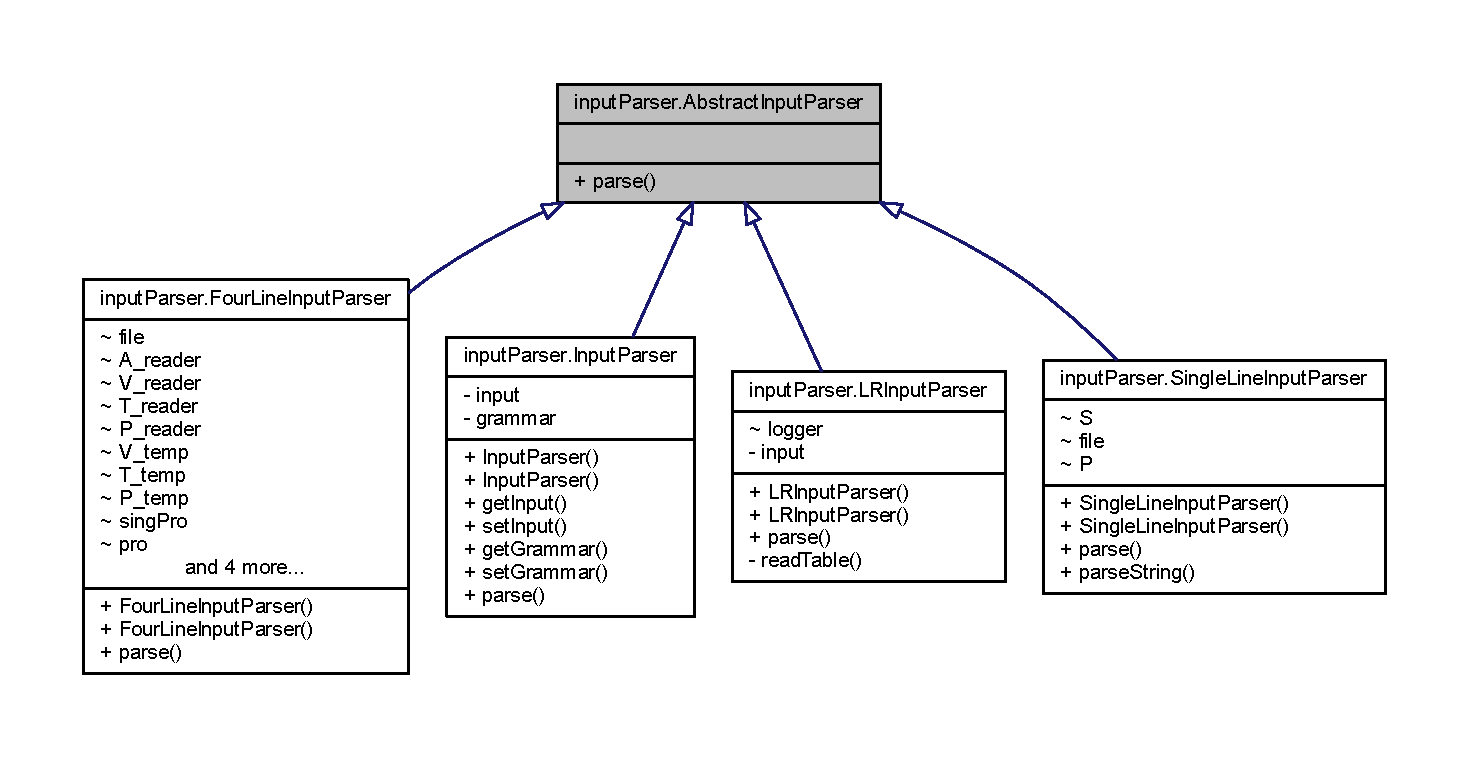
\includegraphics[width=350pt]{classinput_parser_1_1_abstract_input_parser__inherit__graph}
\end{center}
\end{figure}
\subsection*{Public Member Functions}
\begin{DoxyCompactItemize}
\item 
abstract Object \hyperlink{classinput_parser_1_1_abstract_input_parser_a548b0f6fa44b7954b79bdd964336bafe}{parse} ()  throws Exception
\begin{DoxyCompactList}\small\item\em Execute the parse operation on the object. \end{DoxyCompactList}\end{DoxyCompactItemize}


\subsection{Detailed Description}


Definition at line 4 of file Abstract\-Input\-Parser.\-java.



\subsection{Member Function Documentation}
\hypertarget{classinput_parser_1_1_abstract_input_parser_a548b0f6fa44b7954b79bdd964336bafe}{\index{input\-Parser\-::\-Abstract\-Input\-Parser@{input\-Parser\-::\-Abstract\-Input\-Parser}!parse@{parse}}
\index{parse@{parse}!inputParser::AbstractInputParser@{input\-Parser\-::\-Abstract\-Input\-Parser}}
\subsubsection[{parse}]{\setlength{\rightskip}{0pt plus 5cm}abstract Object {\bf input\-Parser.\-Abstract\-Input\-Parser.\-parse} (
\begin{DoxyParamCaption}
{}
\end{DoxyParamCaption}
)  throws Exception\hspace{0.3cm}{\ttfamily  \mbox{[}pure virtual\mbox{]}}}}\label{classinput_parser_1_1_abstract_input_parser_a548b0f6fa44b7954b79bdd964336bafe}


Execute the parse operation on the object. 

\begin{DoxyReturn}{Returns}
the parsing result 
\end{DoxyReturn}

\begin{DoxyExceptions}{Exceptions}
{\em Exception} & \\
\hline
\end{DoxyExceptions}
\begin{DoxyAuthor}{Author}
Paolo Pino 
\end{DoxyAuthor}


Implemented in \hyperlink{classinput_parser_1_1_input_parser_a08cd69f3dbb1be117c45b4ccf5d861e6}{input\-Parser.\-Input\-Parser}, \hyperlink{classinput_parser_1_1_four_line_input_parser_a99c37488d66cfeecb33e13d573b4a81a}{input\-Parser.\-Four\-Line\-Input\-Parser}, \hyperlink{classinput_parser_1_1_single_line_input_parser_ad822676b0d3182a591e2004c3bcc79d5}{input\-Parser.\-Single\-Line\-Input\-Parser}, and \hyperlink{classinput_parser_1_1_l_r_input_parser_ad81d1510d9b12b4b8b2dedbe117e88c1}{input\-Parser.\-L\-R\-Input\-Parser}.



Here is the caller graph for this function\-:
\nopagebreak
\begin{figure}[H]
\begin{center}
\leavevmode
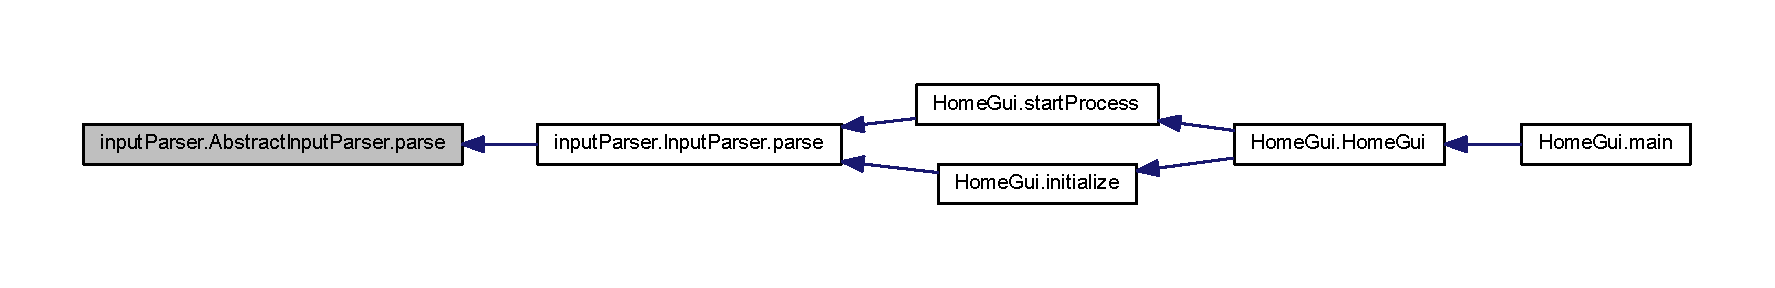
\includegraphics[width=350pt]{classinput_parser_1_1_abstract_input_parser_a548b0f6fa44b7954b79bdd964336bafe_icgraph}
\end{center}
\end{figure}




The documentation for this class was generated from the following file\-:\begin{DoxyCompactItemize}
\item 
src/input\-Parser/Abstract\-Input\-Parser.\-java\end{DoxyCompactItemize}

\hypertarget{classparser_program_1_1_ast}{\section{parser\-Program.\-Ast Class Reference}
\label{classparser_program_1_1_ast}\index{parser\-Program.\-Ast@{parser\-Program.\-Ast}}
}


Abstract Syntax Three class.  




Collaboration diagram for parser\-Program.\-Ast\-:
\nopagebreak
\begin{figure}[H]
\begin{center}
\leavevmode
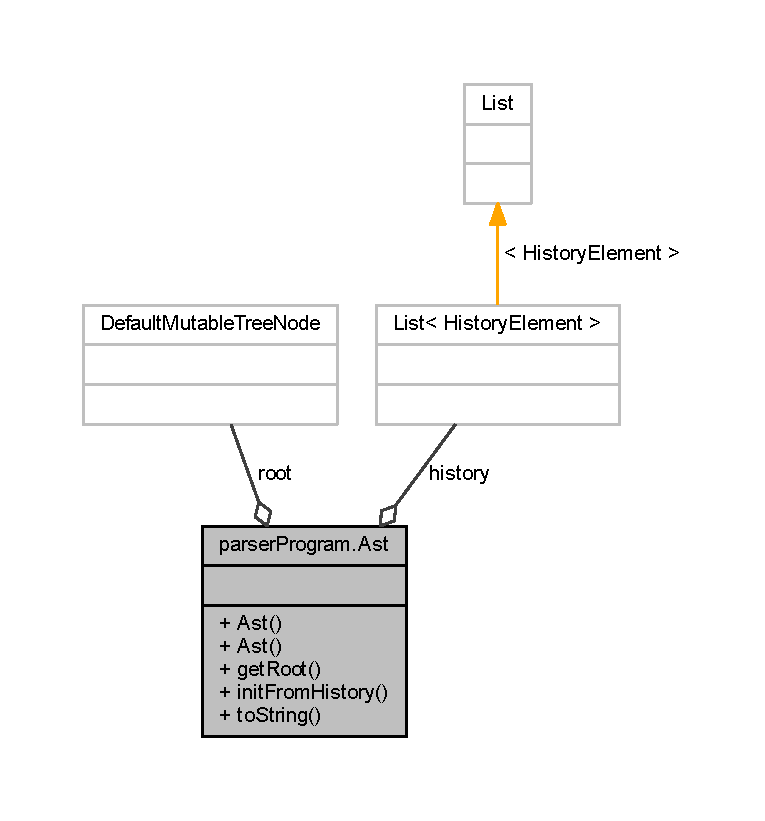
\includegraphics[width=350pt]{classparser_program_1_1_ast__coll__graph}
\end{center}
\end{figure}
\subsection*{Public Member Functions}
\begin{DoxyCompactItemize}
\item 
\hypertarget{classparser_program_1_1_ast_ae717a4491faf02f3753ad055eec6d5dd}{\hyperlink{classparser_program_1_1_ast_ae717a4491faf02f3753ad055eec6d5dd}{Ast} ()}\label{classparser_program_1_1_ast_ae717a4491faf02f3753ad055eec6d5dd}

\begin{DoxyCompactList}\small\item\em Default constructor. \end{DoxyCompactList}\item 
\hyperlink{classparser_program_1_1_ast_a0dd9cc520a52069ec8d2bcccf7567799}{Ast} (List$<$ \hyperlink{classparser_program_1_1_history_element}{History\-Element} $>$ h)
\begin{DoxyCompactList}\small\item\em Construct the object with specified history. \end{DoxyCompactList}\item 
Default\-Mutable\-Tree\-Node \hyperlink{classparser_program_1_1_ast_af586bb4da64c79d9259c87757456d685}{get\-Root} ()
\item 
void \hyperlink{classparser_program_1_1_ast_a9ad5f3d77935440489df31131b18bf8e}{init\-From\-History} ()  throws Exception
\begin{DoxyCompactList}\small\item\em Initialize the three from the parsing history. \end{DoxyCompactList}\item 
\hypertarget{classparser_program_1_1_ast_a58d8cf855d692e96d5af5d49a8bca4b9}{String {\bfseries to\-String} ()}\label{classparser_program_1_1_ast_a58d8cf855d692e96d5af5d49a8bca4b9}

\end{DoxyCompactItemize}
\subsection*{Private Attributes}
\begin{DoxyCompactItemize}
\item 
\hypertarget{classparser_program_1_1_ast_a565a13f94f478e998401f7abc25643aa}{List$<$ \hyperlink{classparser_program_1_1_history_element}{History\-Element} $>$ \hyperlink{classparser_program_1_1_ast_a565a13f94f478e998401f7abc25643aa}{history}}\label{classparser_program_1_1_ast_a565a13f94f478e998401f7abc25643aa}

\begin{DoxyCompactList}\small\item\em the chronology of parsing \end{DoxyCompactList}\item 
\hypertarget{classparser_program_1_1_ast_a004223ce41eed0c97a6fb63449b4b836}{Default\-Mutable\-Tree\-Node \hyperlink{classparser_program_1_1_ast_a004223ce41eed0c97a6fb63449b4b836}{root}}\label{classparser_program_1_1_ast_a004223ce41eed0c97a6fb63449b4b836}

\begin{DoxyCompactList}\small\item\em the root of the three \end{DoxyCompactList}\end{DoxyCompactItemize}


\subsection{Detailed Description}
Abstract Syntax Three class. 

\begin{DoxyAuthor}{Author}
Paolo Pino 
\end{DoxyAuthor}


Definition at line 11 of file Ast.\-java.



\subsection{Constructor \& Destructor Documentation}
\hypertarget{classparser_program_1_1_ast_a0dd9cc520a52069ec8d2bcccf7567799}{\index{parser\-Program\-::\-Ast@{parser\-Program\-::\-Ast}!Ast@{Ast}}
\index{Ast@{Ast}!parserProgram::Ast@{parser\-Program\-::\-Ast}}
\subsubsection[{Ast}]{\setlength{\rightskip}{0pt plus 5cm}{\bf parser\-Program.\-Ast.\-Ast} (
\begin{DoxyParamCaption}
\item[{List$<$ {\bf History\-Element} $>$}]{h}
\end{DoxyParamCaption}
)}}\label{classparser_program_1_1_ast_a0dd9cc520a52069ec8d2bcccf7567799}


Construct the object with specified history. 


\begin{DoxyParams}{Parameters}
{\em h} & history \\
\hline
\end{DoxyParams}


Definition at line 29 of file Ast.\-java.



\subsection{Member Function Documentation}
\hypertarget{classparser_program_1_1_ast_af586bb4da64c79d9259c87757456d685}{\index{parser\-Program\-::\-Ast@{parser\-Program\-::\-Ast}!get\-Root@{get\-Root}}
\index{get\-Root@{get\-Root}!parserProgram::Ast@{parser\-Program\-::\-Ast}}
\subsubsection[{get\-Root}]{\setlength{\rightskip}{0pt plus 5cm}Default\-Mutable\-Tree\-Node {\bf parser\-Program.\-Ast.\-get\-Root} (
\begin{DoxyParamCaption}
{}
\end{DoxyParamCaption}
)}}\label{classparser_program_1_1_ast_af586bb4da64c79d9259c87757456d685}
\begin{DoxyReturn}{Returns}
the root of the three. 
\end{DoxyReturn}


Definition at line 38 of file Ast.\-java.



Here is the caller graph for this function\-:
\nopagebreak
\begin{figure}[H]
\begin{center}
\leavevmode
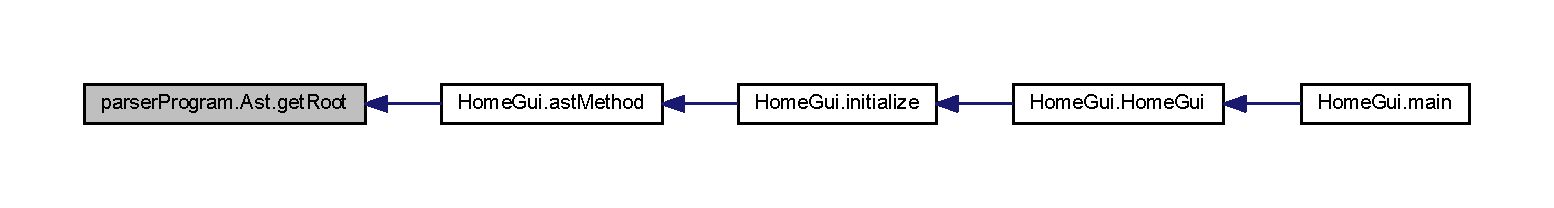
\includegraphics[width=350pt]{classparser_program_1_1_ast_af586bb4da64c79d9259c87757456d685_icgraph}
\end{center}
\end{figure}


\hypertarget{classparser_program_1_1_ast_a9ad5f3d77935440489df31131b18bf8e}{\index{parser\-Program\-::\-Ast@{parser\-Program\-::\-Ast}!init\-From\-History@{init\-From\-History}}
\index{init\-From\-History@{init\-From\-History}!parserProgram::Ast@{parser\-Program\-::\-Ast}}
\subsubsection[{init\-From\-History}]{\setlength{\rightskip}{0pt plus 5cm}void {\bf parser\-Program.\-Ast.\-init\-From\-History} (
\begin{DoxyParamCaption}
{}
\end{DoxyParamCaption}
)  throws Exception}}\label{classparser_program_1_1_ast_a9ad5f3d77935440489df31131b18bf8e}


Initialize the three from the parsing history. 


\begin{DoxyExceptions}{Exceptions}
{\em Exception} & if error. \\
\hline
\end{DoxyExceptions}


Definition at line 46 of file Ast.\-java.



Here is the caller graph for this function\-:
\nopagebreak
\begin{figure}[H]
\begin{center}
\leavevmode
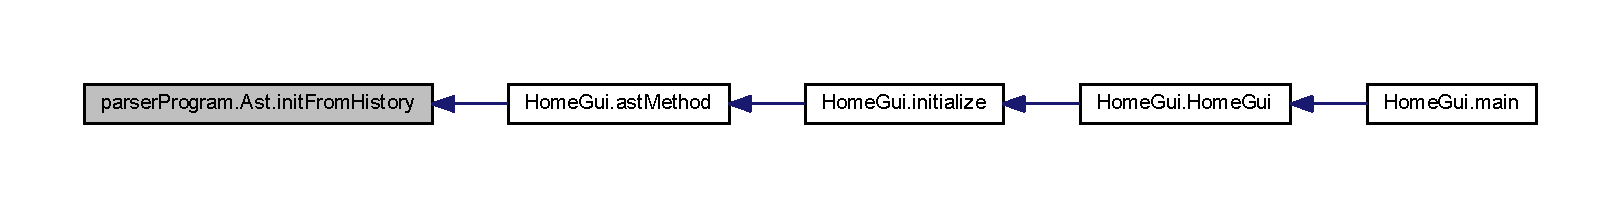
\includegraphics[width=350pt]{classparser_program_1_1_ast_a9ad5f3d77935440489df31131b18bf8e_icgraph}
\end{center}
\end{figure}




The documentation for this class was generated from the following file\-:\begin{DoxyCompactItemize}
\item 
src/parser\-Program/Ast.\-java\end{DoxyCompactItemize}

\hypertarget{classcontext_free_1_1parser_1_1_automa}{\section{context\-Free.\-parser.\-Automa Class Reference}
\label{classcontext_free_1_1parser_1_1_automa}\index{context\-Free.\-parser.\-Automa@{context\-Free.\-parser.\-Automa}}
}


Collaboration diagram for context\-Free.\-parser.\-Automa\-:\nopagebreak
\begin{figure}[H]
\begin{center}
\leavevmode
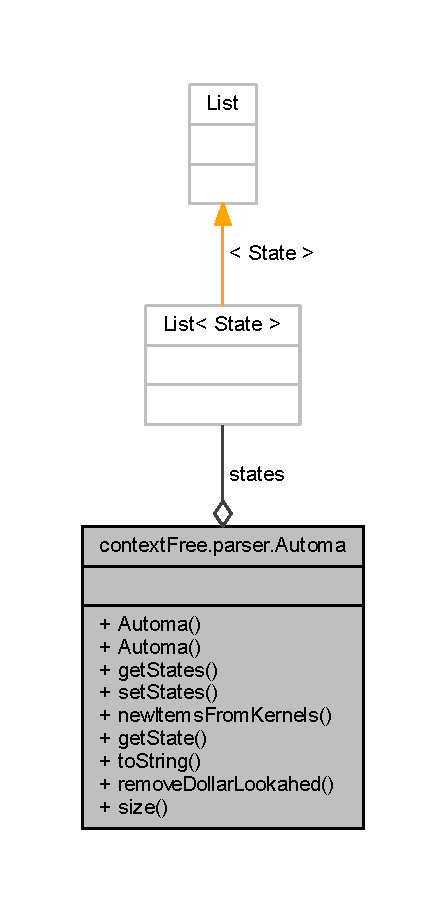
\includegraphics[width=214pt]{classcontext_free_1_1parser_1_1_automa__coll__graph}
\end{center}
\end{figure}
\subsection*{Public Member Functions}
\begin{DoxyCompactItemize}
\item 
\hypertarget{classcontext_free_1_1parser_1_1_automa_a6a030d3a01bf7ef99b437fcf14727bad}{{\bfseries Automa} (List$<$ \hyperlink{classcontext_free_1_1parser_1_1_state}{State} $>$ states)}\label{classcontext_free_1_1parser_1_1_automa_a6a030d3a01bf7ef99b437fcf14727bad}

\item 
\hypertarget{classcontext_free_1_1parser_1_1_automa_a0a2be97fe40e3035c579b83535649c2e}{List$<$ \hyperlink{classcontext_free_1_1parser_1_1_state}{State} $>$ {\bfseries get\-States} ()}\label{classcontext_free_1_1parser_1_1_automa_a0a2be97fe40e3035c579b83535649c2e}

\item 
\hypertarget{classcontext_free_1_1parser_1_1_automa_a16f74867e919ccddf13441295c80295b}{void {\bfseries set\-States} (List$<$ \hyperlink{classcontext_free_1_1parser_1_1_state}{State} $>$ states)}\label{classcontext_free_1_1parser_1_1_automa_a16f74867e919ccddf13441295c80295b}

\item 
List$<$ \hyperlink{classcontext_free_1_1parser_1_1_state}{State} $>$ \hyperlink{classcontext_free_1_1parser_1_1_automa_ad82cfb3bb6b22d084ef18a95350828b3}{new\-Items\-From\-Kernels} ()
\begin{DoxyCompactList}\small\item\em Get kernels element for each states into automa. \end{DoxyCompactList}\item 
\hyperlink{classcontext_free_1_1parser_1_1_state}{State} \hyperlink{classcontext_free_1_1parser_1_1_automa_a08b46ef04492599b98660a5e55f356bd}{get\-State} (int i)
\begin{DoxyCompactList}\small\item\em Return a state with a specific state index. \end{DoxyCompactList}\item 
\hypertarget{classcontext_free_1_1parser_1_1_automa_a816d25575a45d9a0bbc415a6e0a71a2e}{String {\bfseries to\-String} ()}\label{classcontext_free_1_1parser_1_1_automa_a816d25575a45d9a0bbc415a6e0a71a2e}

\item 
void \hyperlink{classcontext_free_1_1parser_1_1_automa_ad94ecd3a9f8850220f86b6c54b751f78}{remove\-Dollar\-Lookahed} ()
\begin{DoxyCompactList}\small\item\em remove dollar simbol lookahed \end{DoxyCompactList}\item 
\hypertarget{classcontext_free_1_1parser_1_1_automa_aa3e53614ea757f72b87144aa6b5b2282}{int {\bfseries size} ()}\label{classcontext_free_1_1parser_1_1_automa_aa3e53614ea757f72b87144aa6b5b2282}

\end{DoxyCompactItemize}
\subsection*{Private Attributes}
\begin{DoxyCompactItemize}
\item 
\hypertarget{classcontext_free_1_1parser_1_1_automa_a5b71afafd71dfa903e36c786618b556d}{List$<$ \hyperlink{classcontext_free_1_1parser_1_1_state}{State} $>$ {\bfseries states}}\label{classcontext_free_1_1parser_1_1_automa_a5b71afafd71dfa903e36c786618b556d}

\end{DoxyCompactItemize}


\subsection{Detailed Description}


Definition at line 6 of file Automa.\-java.



\subsection{Member Function Documentation}
\hypertarget{classcontext_free_1_1parser_1_1_automa_a08b46ef04492599b98660a5e55f356bd}{\index{context\-Free\-::parser\-::\-Automa@{context\-Free\-::parser\-::\-Automa}!get\-State@{get\-State}}
\index{get\-State@{get\-State}!contextFree::parser::Automa@{context\-Free\-::parser\-::\-Automa}}
\subsubsection[{get\-State}]{\setlength{\rightskip}{0pt plus 5cm}{\bf State} {\bf context\-Free.\-parser.\-Automa.\-get\-State} (
\begin{DoxyParamCaption}
\item[{int}]{i}
\end{DoxyParamCaption}
)}}\label{classcontext_free_1_1parser_1_1_automa_a08b46ef04492599b98660a5e55f356bd}


Return a state with a specific state index. 

\begin{DoxyVerb}  @param i the index of desired state
\end{DoxyVerb}
 \begin{DoxyReturn}{Returns}
the \hyperlink{classcontext_free_1_1parser_1_1_state}{State} reference if the state exist else null; 
\end{DoxyReturn}


Definition at line 42 of file Automa.\-java.

\hypertarget{classcontext_free_1_1parser_1_1_automa_ad82cfb3bb6b22d084ef18a95350828b3}{\index{context\-Free\-::parser\-::\-Automa@{context\-Free\-::parser\-::\-Automa}!new\-Items\-From\-Kernels@{new\-Items\-From\-Kernels}}
\index{new\-Items\-From\-Kernels@{new\-Items\-From\-Kernels}!contextFree::parser::Automa@{context\-Free\-::parser\-::\-Automa}}
\subsubsection[{new\-Items\-From\-Kernels}]{\setlength{\rightskip}{0pt plus 5cm}List$<${\bf State}$>$ {\bf context\-Free.\-parser.\-Automa.\-new\-Items\-From\-Kernels} (
\begin{DoxyParamCaption}
{}
\end{DoxyParamCaption}
)}}\label{classcontext_free_1_1parser_1_1_automa_ad82cfb3bb6b22d084ef18a95350828b3}


Get kernels element for each states into automa. 

\begin{DoxyReturn}{Returns}
new \hyperlink{classcontext_free_1_1parser_1_1_state}{State} list with shift value and kernel item only 
\end{DoxyReturn}


Definition at line 28 of file Automa.\-java.



Here is the caller graph for this function\-:\nopagebreak
\begin{figure}[H]
\begin{center}
\leavevmode
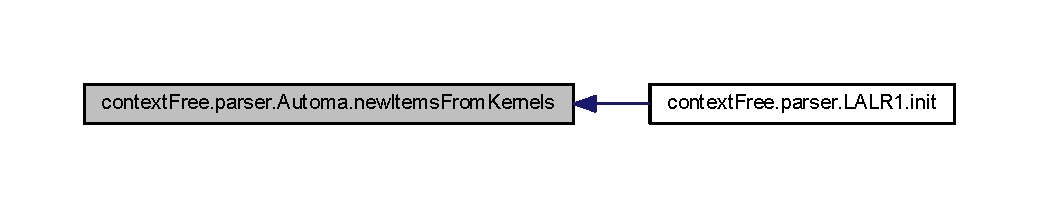
\includegraphics[width=350pt]{classcontext_free_1_1parser_1_1_automa_ad82cfb3bb6b22d084ef18a95350828b3_icgraph}
\end{center}
\end{figure}


\hypertarget{classcontext_free_1_1parser_1_1_automa_ad94ecd3a9f8850220f86b6c54b751f78}{\index{context\-Free\-::parser\-::\-Automa@{context\-Free\-::parser\-::\-Automa}!remove\-Dollar\-Lookahed@{remove\-Dollar\-Lookahed}}
\index{remove\-Dollar\-Lookahed@{remove\-Dollar\-Lookahed}!contextFree::parser::Automa@{context\-Free\-::parser\-::\-Automa}}
\subsubsection[{remove\-Dollar\-Lookahed}]{\setlength{\rightskip}{0pt plus 5cm}void {\bf context\-Free.\-parser.\-Automa.\-remove\-Dollar\-Lookahed} (
\begin{DoxyParamCaption}
{}
\end{DoxyParamCaption}
)}}\label{classcontext_free_1_1parser_1_1_automa_ad94ecd3a9f8850220f86b6c54b751f78}


remove dollar simbol lookahed 

\begin{DoxyAuthor}{Author}
Paolo Pino 
\end{DoxyAuthor}


Definition at line 60 of file Automa.\-java.



Here is the caller graph for this function\-:\nopagebreak
\begin{figure}[H]
\begin{center}
\leavevmode
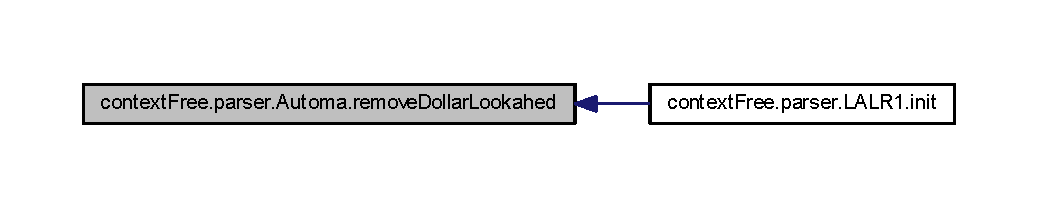
\includegraphics[width=350pt]{classcontext_free_1_1parser_1_1_automa_ad94ecd3a9f8850220f86b6c54b751f78_icgraph}
\end{center}
\end{figure}




The documentation for this class was generated from the following file\-:\begin{DoxyCompactItemize}
\item 
src/context\-Free/parser/Automa.\-java\end{DoxyCompactItemize}

\hypertarget{classinput_parser_1_1_concrete_parser_factory}{\section{input\-Parser.\-Concrete\-Parser\-Factory Class Reference}
\label{classinput_parser_1_1_concrete_parser_factory}\index{input\-Parser.\-Concrete\-Parser\-Factory@{input\-Parser.\-Concrete\-Parser\-Factory}}
}
Inheritance diagram for input\-Parser.\-Concrete\-Parser\-Factory\-:\begin{figure}[H]
\begin{center}
\leavevmode
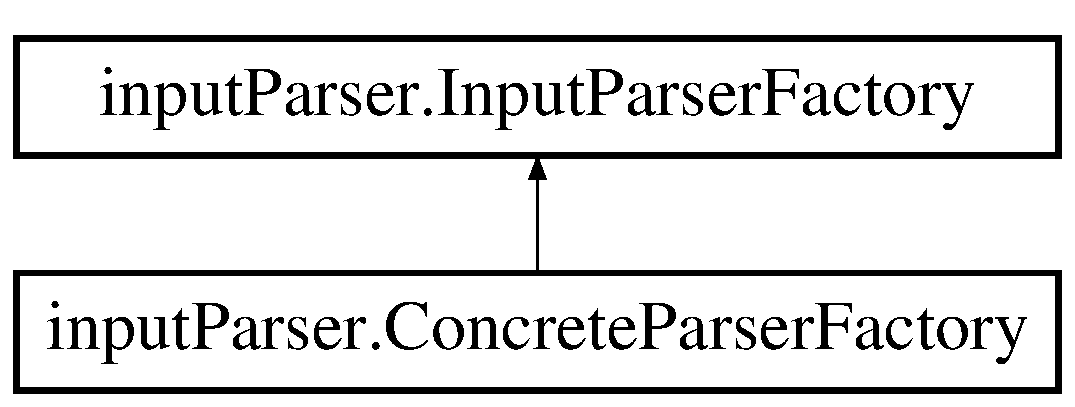
\includegraphics[height=2.000000cm]{classinput_parser_1_1_concrete_parser_factory}
\end{center}
\end{figure}
\subsection*{Protected Member Functions}
\begin{DoxyCompactItemize}
\item 
\hyperlink{classinput_parser_1_1_input_parser}{Input\-Parser} \hyperlink{classinput_parser_1_1_concrete_parser_factory_a022ebe49ba99090793ad4a10b3f8fbfe}{factory\-Method} (String in)
\end{DoxyCompactItemize}


\subsection{Detailed Description}


Definition at line 7 of file Concrete\-Parser\-Factory.\-java.



\subsection{Member Function Documentation}
\hypertarget{classinput_parser_1_1_concrete_parser_factory_a022ebe49ba99090793ad4a10b3f8fbfe}{\index{input\-Parser\-::\-Concrete\-Parser\-Factory@{input\-Parser\-::\-Concrete\-Parser\-Factory}!factory\-Method@{factory\-Method}}
\index{factory\-Method@{factory\-Method}!inputParser::ConcreteParserFactory@{input\-Parser\-::\-Concrete\-Parser\-Factory}}
\subsubsection[{factory\-Method}]{\setlength{\rightskip}{0pt plus 5cm}{\bf Input\-Parser} {\bf input\-Parser.\-Concrete\-Parser\-Factory.\-factory\-Method} (
\begin{DoxyParamCaption}
\item[{String}]{in}
\end{DoxyParamCaption}
)\hspace{0.3cm}{\ttfamily  \mbox{[}protected, virtual\mbox{]}}}}\label{classinput_parser_1_1_concrete_parser_factory_a022ebe49ba99090793ad4a10b3f8fbfe}


Implements \hyperlink{classinput_parser_1_1_parser_factory_a3c9d82a4912ea351eefd5d943d5af35c}{input\-Parser.\-Parser\-Factory}.



Definition at line 10 of file Concrete\-Parser\-Factory.\-java.



The documentation for this class was generated from the following file\-:\begin{DoxyCompactItemize}
\item 
src/input\-Parser/\hyperlink{_concrete_parser_factory_8java}{Concrete\-Parser\-Factory.\-java}\end{DoxyCompactItemize}

\hypertarget{classcontext_free_1_1grammar_1_1_context_free_grammar}{\section{context\-Free.\-grammar.\-Context\-Free\-Grammar Class Reference}
\label{classcontext_free_1_1grammar_1_1_context_free_grammar}\index{context\-Free.\-grammar.\-Context\-Free\-Grammar@{context\-Free.\-grammar.\-Context\-Free\-Grammar}}
}


Define a context-\/free grammar type.  




Inheritance diagram for context\-Free.\-grammar.\-Context\-Free\-Grammar\-:
\nopagebreak
\begin{figure}[H]
\begin{center}
\leavevmode
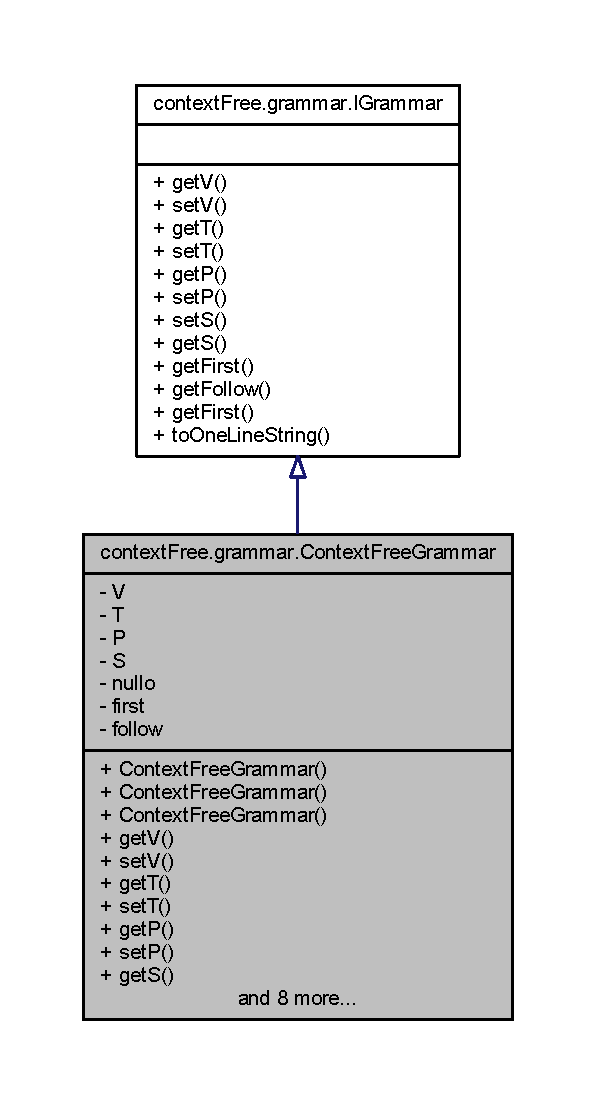
\includegraphics[width=286pt]{classcontext_free_1_1grammar_1_1_context_free_grammar__inherit__graph}
\end{center}
\end{figure}


Collaboration diagram for context\-Free.\-grammar.\-Context\-Free\-Grammar\-:
\nopagebreak
\begin{figure}[H]
\begin{center}
\leavevmode
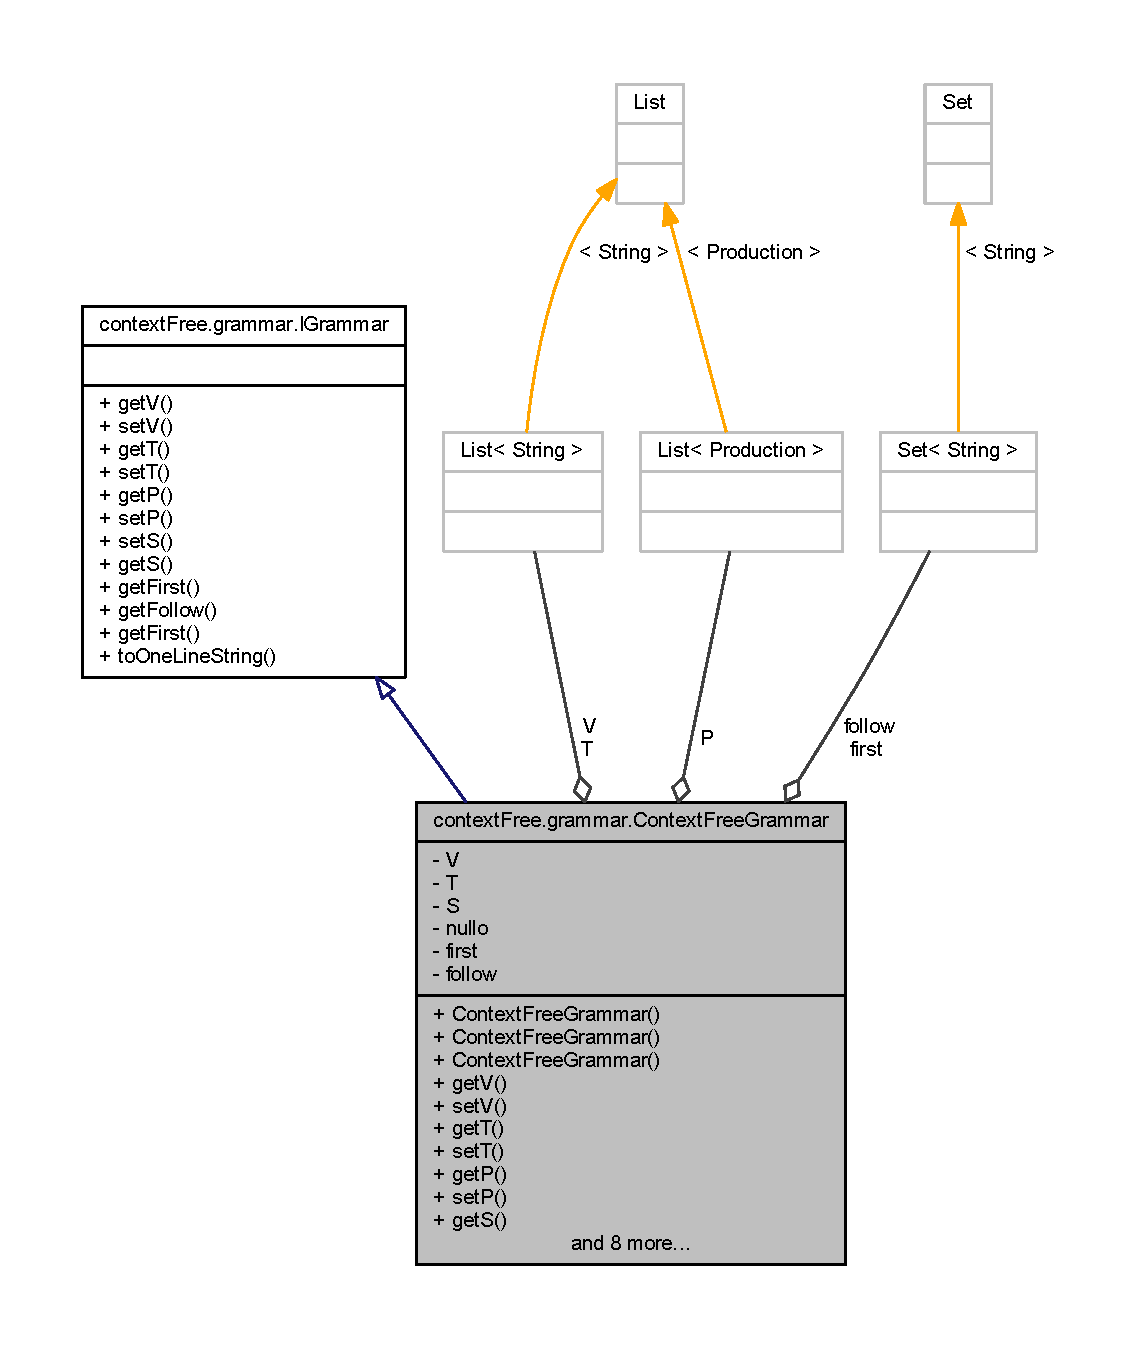
\includegraphics[width=350pt]{classcontext_free_1_1grammar_1_1_context_free_grammar__coll__graph}
\end{center}
\end{figure}
\subsection*{Public Member Functions}
\begin{DoxyCompactItemize}
\item 
\hypertarget{classcontext_free_1_1grammar_1_1_context_free_grammar_ad4871f790005d3582e0f4d50aceac810}{{\bfseries Context\-Free\-Grammar} (String ass, List$<$ \hyperlink{classcontext_free_1_1grammar_1_1_production}{Production} $>$ prod)}\label{classcontext_free_1_1grammar_1_1_context_free_grammar_ad4871f790005d3582e0f4d50aceac810}

\item 
\hypertarget{classcontext_free_1_1grammar_1_1_context_free_grammar_aa29c85cc857ff390f50efc82d7c959e9}{{\bfseries Context\-Free\-Grammar} (String ass, List$<$ \hyperlink{classcontext_free_1_1grammar_1_1_production}{Production} $>$ prod, List$<$ String $>$ V, List$<$ String $>$ T)}\label{classcontext_free_1_1grammar_1_1_context_free_grammar_aa29c85cc857ff390f50efc82d7c959e9}

\item 
List$<$ String $>$ \hyperlink{classcontext_free_1_1grammar_1_1_context_free_grammar_a664b69a446100c7c4e7a390fb2ee5ebc}{get\-V} ()
\begin{DoxyCompactList}\small\item\em Get non-\/terminal symbols list. \end{DoxyCompactList}\item 
void \hyperlink{classcontext_free_1_1grammar_1_1_context_free_grammar_ad3d3e1efadeb4cc6ed252342fd52c76c}{set\-V} (List$<$ String $>$ v)
\begin{DoxyCompactList}\small\item\em Set the list of non-\/terminal symbols. \end{DoxyCompactList}\item 
List$<$ String $>$ \hyperlink{classcontext_free_1_1grammar_1_1_context_free_grammar_a75f1bbf1e0d1d1350032c628779fcffd}{get\-T} ()
\begin{DoxyCompactList}\small\item\em Get terminal symbols list. \end{DoxyCompactList}\item 
void \hyperlink{classcontext_free_1_1grammar_1_1_context_free_grammar_aa1c9a277d660b2ba8443f47cb9543811}{set\-T} (List$<$ String $>$ e)
\begin{DoxyCompactList}\small\item\em Set the list of terminal symbols. \end{DoxyCompactList}\item 
List$<$ \hyperlink{classcontext_free_1_1grammar_1_1_production}{Production} $>$ \hyperlink{classcontext_free_1_1grammar_1_1_context_free_grammar_ad00a00b018844cf2acb0c1c5f5d97468}{get\-P} ()
\begin{DoxyCompactList}\small\item\em Get production list. \end{DoxyCompactList}\item 
void \hyperlink{classcontext_free_1_1grammar_1_1_context_free_grammar_a2a66695521702040224c23898b579c92}{set\-P} (List$<$ \hyperlink{classcontext_free_1_1grammar_1_1_production}{Production} $>$ p)
\begin{DoxyCompactList}\small\item\em Set the produciton list. \end{DoxyCompactList}\item 
String \hyperlink{classcontext_free_1_1grammar_1_1_context_free_grammar_ad278c4f5e2bdec1d011d11a3008d8754}{get\-S} ()
\begin{DoxyCompactList}\small\item\em Get the axioms. \end{DoxyCompactList}\item 
void \hyperlink{classcontext_free_1_1grammar_1_1_context_free_grammar_a2f4c3ec7270d799ed127cb162e0213b3}{set\-S} (String s)
\begin{DoxyCompactList}\small\item\em Set the axioms for the grammar. \end{DoxyCompactList}\item 
Set$<$ String $>$\mbox{[}$\,$\mbox{]} \hyperlink{classcontext_free_1_1grammar_1_1_context_free_grammar_adc3a25917132474960be34329cdaead9}{get\-First} ()
\begin{DoxyCompactList}\small\item\em Get the list of first for the grammar. \end{DoxyCompactList}\item 
Set$<$ String $>$ \hyperlink{classcontext_free_1_1grammar_1_1_context_free_grammar_a2140cdc636585e9714e8dc42c936eee5}{get\-First} (String A)
\begin{DoxyCompactList}\small\item\em I spent a character returns the first list associated to it. \end{DoxyCompactList}\item 
Set$<$ String $>$\mbox{[}$\,$\mbox{]} \hyperlink{classcontext_free_1_1grammar_1_1_context_free_grammar_a5dae0e5de95349d310869fb5941cb5be}{get\-Follow} ()
\begin{DoxyCompactList}\small\item\em I spent a character returns the Follow list associated to it. \end{DoxyCompactList}\item 
void \hyperlink{classcontext_free_1_1grammar_1_1_context_free_grammar_ac880ed3ca36ddcd8e20d8279af08244d}{nullo} ()
\begin{DoxyCompactList}\small\item\em population structure Bolean \mbox{[}\mbox{]} null defined in class grammar, it has the same size of V. \end{DoxyCompactList}\item 
void \hyperlink{classcontext_free_1_1grammar_1_1_context_free_grammar_a9c3bfe0b038204420b470fab326ce7bb}{first} ()
\begin{DoxyCompactList}\small\item\em Populate structure in Set$<$\-String$>$\mbox{[}\mbox{]}first for each non-\/terminal V, using a structure of type Set to avoid duplication. \end{DoxyCompactList}\item 
void \hyperlink{classcontext_free_1_1grammar_1_1_context_free_grammar_aca5cad8fa908f908d38e0e7e0aa181ed}{follow} ()
\begin{DoxyCompactList}\small\item\em Population structure in Set $<$\-String$>$ \mbox{[}\mbox{]} first for each non-\/terminal V, using a structure of type Set to avoid duplication. \end{DoxyCompactList}\item 
\hypertarget{classcontext_free_1_1grammar_1_1_context_free_grammar_afd242bd888b53c20465c0bd3675d29d4}{String {\bfseries to\-String} ()}\label{classcontext_free_1_1grammar_1_1_context_free_grammar_afd242bd888b53c20465c0bd3675d29d4}

\item 
String \hyperlink{classcontext_free_1_1grammar_1_1_context_free_grammar_a922203e2db862d2a8ab31e8e7736273b}{to\-One\-Line\-String} ()
\end{DoxyCompactItemize}
\subsection*{Private Attributes}
\begin{DoxyCompactItemize}
\item 
\hypertarget{classcontext_free_1_1grammar_1_1_context_free_grammar_a8cecf8ee3fe6ca01f58aacf390720746}{List$<$ String $>$ {\bfseries V}}\label{classcontext_free_1_1grammar_1_1_context_free_grammar_a8cecf8ee3fe6ca01f58aacf390720746}

\item 
\hypertarget{classcontext_free_1_1grammar_1_1_context_free_grammar_a5e6072d2c2f11703160c3c39c2968489}{List$<$ String $>$ {\bfseries T}}\label{classcontext_free_1_1grammar_1_1_context_free_grammar_a5e6072d2c2f11703160c3c39c2968489}

\item 
\hypertarget{classcontext_free_1_1grammar_1_1_context_free_grammar_ae1f4363ca57c34622cdca5175aef6b6c}{List$<$ \hyperlink{classcontext_free_1_1grammar_1_1_production}{Production} $>$ {\bfseries P}}\label{classcontext_free_1_1grammar_1_1_context_free_grammar_ae1f4363ca57c34622cdca5175aef6b6c}

\item 
\hypertarget{classcontext_free_1_1grammar_1_1_context_free_grammar_a516b9fb1183524ea3e7859b41f60ad32}{String {\bfseries S}}\label{classcontext_free_1_1grammar_1_1_context_free_grammar_a516b9fb1183524ea3e7859b41f60ad32}

\item 
\hypertarget{classcontext_free_1_1grammar_1_1_context_free_grammar_a5a9f69817c82b19b21adb85326d60f3b}{boolean\mbox{[}$\,$\mbox{]} {\bfseries nullo}}\label{classcontext_free_1_1grammar_1_1_context_free_grammar_a5a9f69817c82b19b21adb85326d60f3b}

\item 
\hypertarget{classcontext_free_1_1grammar_1_1_context_free_grammar_a670c2e35761e57add4c2f3ae29131325}{Set$<$ String $>$\mbox{[}$\,$\mbox{]} {\bfseries first}}\label{classcontext_free_1_1grammar_1_1_context_free_grammar_a670c2e35761e57add4c2f3ae29131325}

\item 
\hypertarget{classcontext_free_1_1grammar_1_1_context_free_grammar_a56137caac336fd26652d4c21252fd95f}{Set$<$ String $>$\mbox{[}$\,$\mbox{]} {\bfseries follow}}\label{classcontext_free_1_1grammar_1_1_context_free_grammar_a56137caac336fd26652d4c21252fd95f}

\end{DoxyCompactItemize}


\subsection{Detailed Description}
Define a context-\/free grammar type. 

\begin{DoxyAuthor}{Author}
Paolo Pino 
\end{DoxyAuthor}


Definition at line 15 of file Context\-Free\-Grammar.\-java.



\subsection{Member Function Documentation}
\hypertarget{classcontext_free_1_1grammar_1_1_context_free_grammar_a9c3bfe0b038204420b470fab326ce7bb}{\index{context\-Free\-::grammar\-::\-Context\-Free\-Grammar@{context\-Free\-::grammar\-::\-Context\-Free\-Grammar}!first@{first}}
\index{first@{first}!contextFree::grammar::ContextFreeGrammar@{context\-Free\-::grammar\-::\-Context\-Free\-Grammar}}
\subsubsection[{first}]{\setlength{\rightskip}{0pt plus 5cm}void context\-Free.\-grammar.\-Context\-Free\-Grammar.\-first (
\begin{DoxyParamCaption}
{}
\end{DoxyParamCaption}
)}}\label{classcontext_free_1_1grammar_1_1_context_free_grammar_a9c3bfe0b038204420b470fab326ce7bb}


Populate structure in Set$<$\-String$>$\mbox{[}\mbox{]}first for each non-\/terminal V, using a structure of type Set to avoid duplication. 

\begin{DoxyAuthor}{Author}
Pierluigi Sottile 
\end{DoxyAuthor}


Definition at line 181 of file Context\-Free\-Grammar.\-java.



Here is the call graph for this function\-:
\nopagebreak
\begin{figure}[H]
\begin{center}
\leavevmode
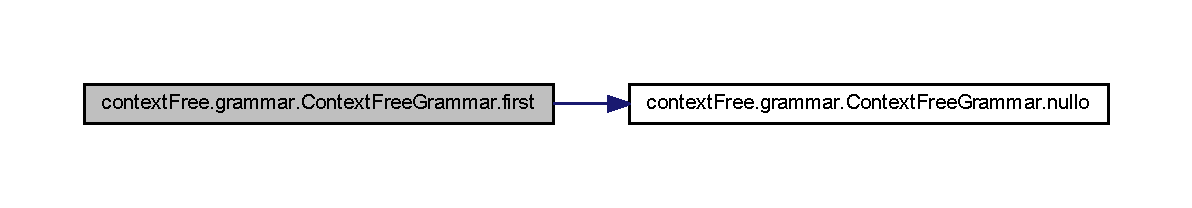
\includegraphics[width=350pt]{classcontext_free_1_1grammar_1_1_context_free_grammar_a9c3bfe0b038204420b470fab326ce7bb_cgraph}
\end{center}
\end{figure}




Here is the caller graph for this function\-:
\nopagebreak
\begin{figure}[H]
\begin{center}
\leavevmode
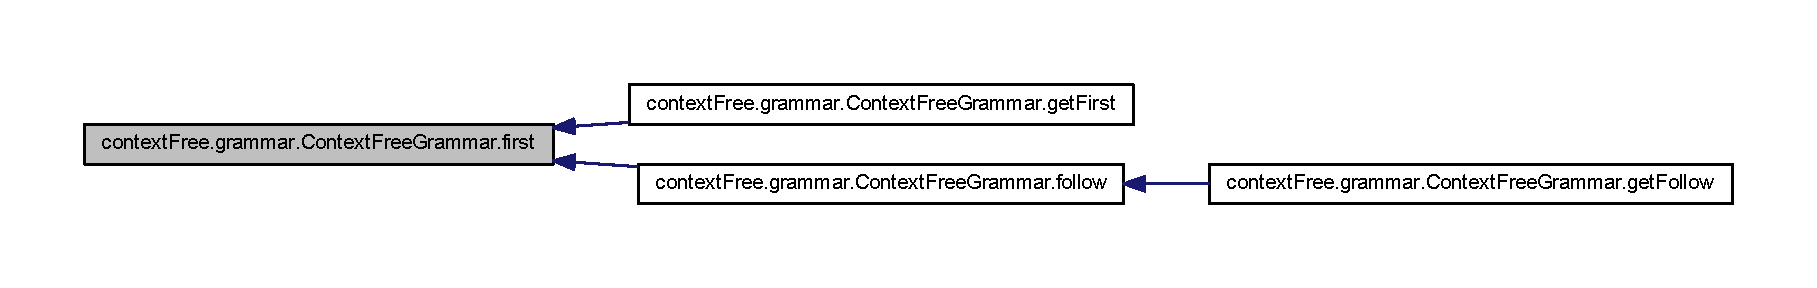
\includegraphics[width=350pt]{classcontext_free_1_1grammar_1_1_context_free_grammar_a9c3bfe0b038204420b470fab326ce7bb_icgraph}
\end{center}
\end{figure}


\hypertarget{classcontext_free_1_1grammar_1_1_context_free_grammar_aca5cad8fa908f908d38e0e7e0aa181ed}{\index{context\-Free\-::grammar\-::\-Context\-Free\-Grammar@{context\-Free\-::grammar\-::\-Context\-Free\-Grammar}!follow@{follow}}
\index{follow@{follow}!contextFree::grammar::ContextFreeGrammar@{context\-Free\-::grammar\-::\-Context\-Free\-Grammar}}
\subsubsection[{follow}]{\setlength{\rightskip}{0pt plus 5cm}void context\-Free.\-grammar.\-Context\-Free\-Grammar.\-follow (
\begin{DoxyParamCaption}
{}
\end{DoxyParamCaption}
)}}\label{classcontext_free_1_1grammar_1_1_context_free_grammar_aca5cad8fa908f908d38e0e7e0aa181ed}


Population structure in Set $<$\-String$>$ \mbox{[}\mbox{]} first for each non-\/terminal V, using a structure of type Set to avoid duplication. 

\begin{DoxyAuthor}{Author}
Pierluigi Sottile 
\end{DoxyAuthor}


Definition at line 249 of file Context\-Free\-Grammar.\-java.



Here is the call graph for this function\-:
\nopagebreak
\begin{figure}[H]
\begin{center}
\leavevmode
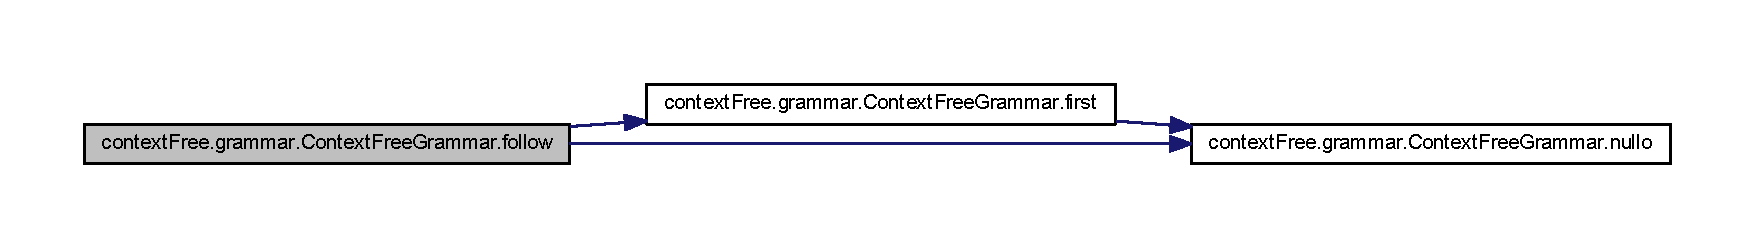
\includegraphics[width=350pt]{classcontext_free_1_1grammar_1_1_context_free_grammar_aca5cad8fa908f908d38e0e7e0aa181ed_cgraph}
\end{center}
\end{figure}




Here is the caller graph for this function\-:
\nopagebreak
\begin{figure}[H]
\begin{center}
\leavevmode
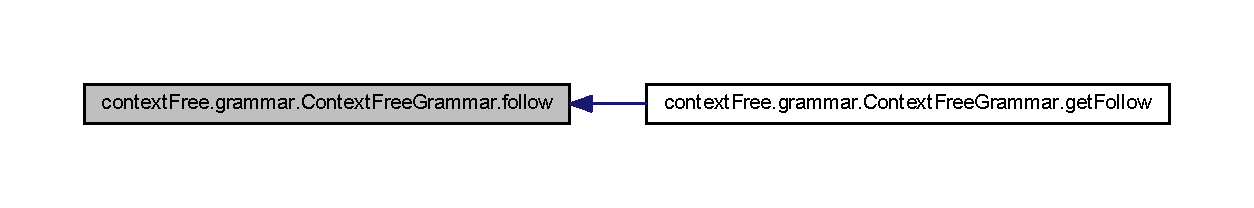
\includegraphics[width=350pt]{classcontext_free_1_1grammar_1_1_context_free_grammar_aca5cad8fa908f908d38e0e7e0aa181ed_icgraph}
\end{center}
\end{figure}


\hypertarget{classcontext_free_1_1grammar_1_1_context_free_grammar_adc3a25917132474960be34329cdaead9}{\index{context\-Free\-::grammar\-::\-Context\-Free\-Grammar@{context\-Free\-::grammar\-::\-Context\-Free\-Grammar}!get\-First@{get\-First}}
\index{get\-First@{get\-First}!contextFree::grammar::ContextFreeGrammar@{context\-Free\-::grammar\-::\-Context\-Free\-Grammar}}
\subsubsection[{get\-First}]{\setlength{\rightskip}{0pt plus 5cm}Set$<$String$>$ \mbox{[}$\,$\mbox{]} {\bf context\-Free.\-grammar.\-Context\-Free\-Grammar.\-get\-First} (
\begin{DoxyParamCaption}
{}
\end{DoxyParamCaption}
)}}\label{classcontext_free_1_1grammar_1_1_context_free_grammar_adc3a25917132474960be34329cdaead9}


Get the list of first for the grammar. 

\begin{DoxyReturn}{Returns}
the first list. 
\end{DoxyReturn}


Implements \hyperlink{interfacecontext_free_1_1grammar_1_1_i_grammar_a256e9280e008a7c709ccb80725ccc0f2}{context\-Free.\-grammar.\-I\-Grammar}.



Definition at line 90 of file Context\-Free\-Grammar.\-java.



Here is the call graph for this function\-:
\nopagebreak
\begin{figure}[H]
\begin{center}
\leavevmode
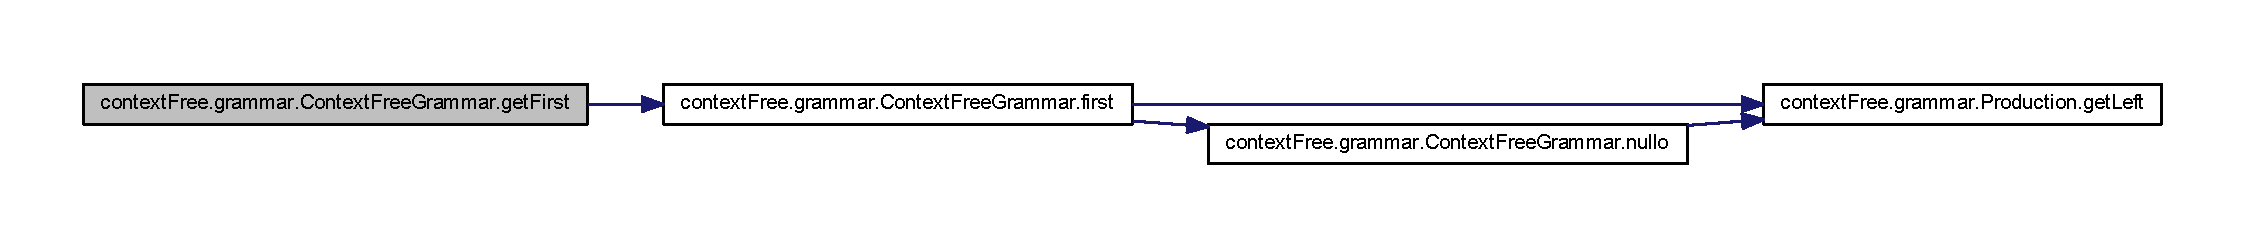
\includegraphics[width=350pt]{classcontext_free_1_1grammar_1_1_context_free_grammar_adc3a25917132474960be34329cdaead9_cgraph}
\end{center}
\end{figure}


\hypertarget{classcontext_free_1_1grammar_1_1_context_free_grammar_a2140cdc636585e9714e8dc42c936eee5}{\index{context\-Free\-::grammar\-::\-Context\-Free\-Grammar@{context\-Free\-::grammar\-::\-Context\-Free\-Grammar}!get\-First@{get\-First}}
\index{get\-First@{get\-First}!contextFree::grammar::ContextFreeGrammar@{context\-Free\-::grammar\-::\-Context\-Free\-Grammar}}
\subsubsection[{get\-First}]{\setlength{\rightskip}{0pt plus 5cm}Set$<$String$>$ {\bf context\-Free.\-grammar.\-Context\-Free\-Grammar.\-get\-First} (
\begin{DoxyParamCaption}
\item[{String}]{A}
\end{DoxyParamCaption}
)}}\label{classcontext_free_1_1grammar_1_1_context_free_grammar_a2140cdc636585e9714e8dc42c936eee5}


I spent a character returns the first list associated to it. 


\begin{DoxyParams}{Parameters}
{\em Simbol} & not-\/\-Terminal A \\
\hline
\end{DoxyParams}
\begin{DoxyReturn}{Returns}
First(\-A) 
\end{DoxyReturn}


Implements \hyperlink{interfacecontext_free_1_1grammar_1_1_i_grammar_a7a05f11e88cdbe29db1849541592e272}{context\-Free.\-grammar.\-I\-Grammar}.



Definition at line 101 of file Context\-Free\-Grammar.\-java.



Here is the call graph for this function\-:
\nopagebreak
\begin{figure}[H]
\begin{center}
\leavevmode
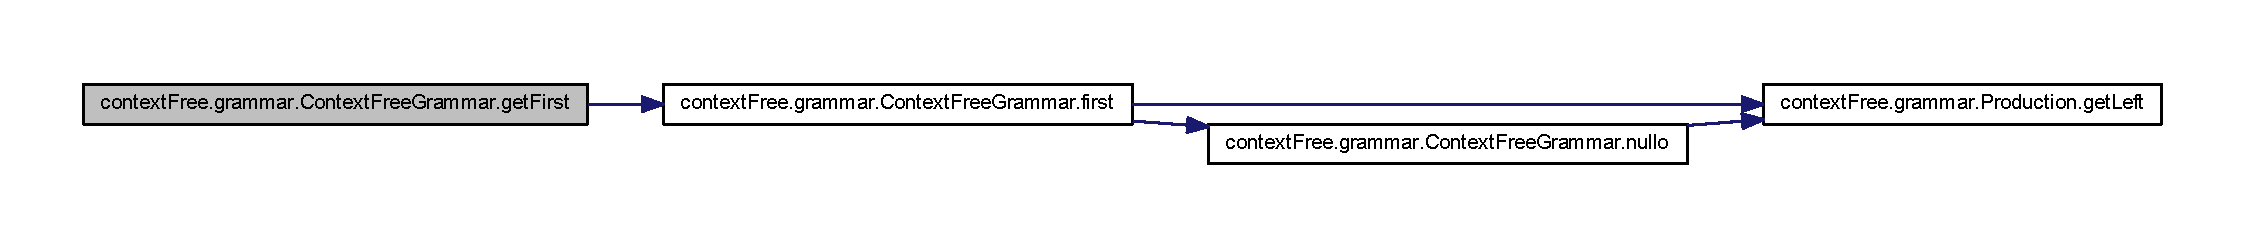
\includegraphics[width=350pt]{classcontext_free_1_1grammar_1_1_context_free_grammar_a2140cdc636585e9714e8dc42c936eee5_cgraph}
\end{center}
\end{figure}


\hypertarget{classcontext_free_1_1grammar_1_1_context_free_grammar_a5dae0e5de95349d310869fb5941cb5be}{\index{context\-Free\-::grammar\-::\-Context\-Free\-Grammar@{context\-Free\-::grammar\-::\-Context\-Free\-Grammar}!get\-Follow@{get\-Follow}}
\index{get\-Follow@{get\-Follow}!contextFree::grammar::ContextFreeGrammar@{context\-Free\-::grammar\-::\-Context\-Free\-Grammar}}
\subsubsection[{get\-Follow}]{\setlength{\rightskip}{0pt plus 5cm}Set$<$String$>$ \mbox{[}$\,$\mbox{]} {\bf context\-Free.\-grammar.\-Context\-Free\-Grammar.\-get\-Follow} (
\begin{DoxyParamCaption}
{}
\end{DoxyParamCaption}
)}}\label{classcontext_free_1_1grammar_1_1_context_free_grammar_a5dae0e5de95349d310869fb5941cb5be}


I spent a character returns the Follow list associated to it. 


\begin{DoxyParams}{Parameters}
{\em Simbol} & not-\/terminal A \\
\hline
\end{DoxyParams}
\begin{DoxyReturn}{Returns}
Follow(\-A) 
\end{DoxyReturn}


Implements \hyperlink{interfacecontext_free_1_1grammar_1_1_i_grammar_aad085d9f84a32ca1abe5fba0c9e5f20c}{context\-Free.\-grammar.\-I\-Grammar}.



Definition at line 110 of file Context\-Free\-Grammar.\-java.



Here is the call graph for this function\-:
\nopagebreak
\begin{figure}[H]
\begin{center}
\leavevmode
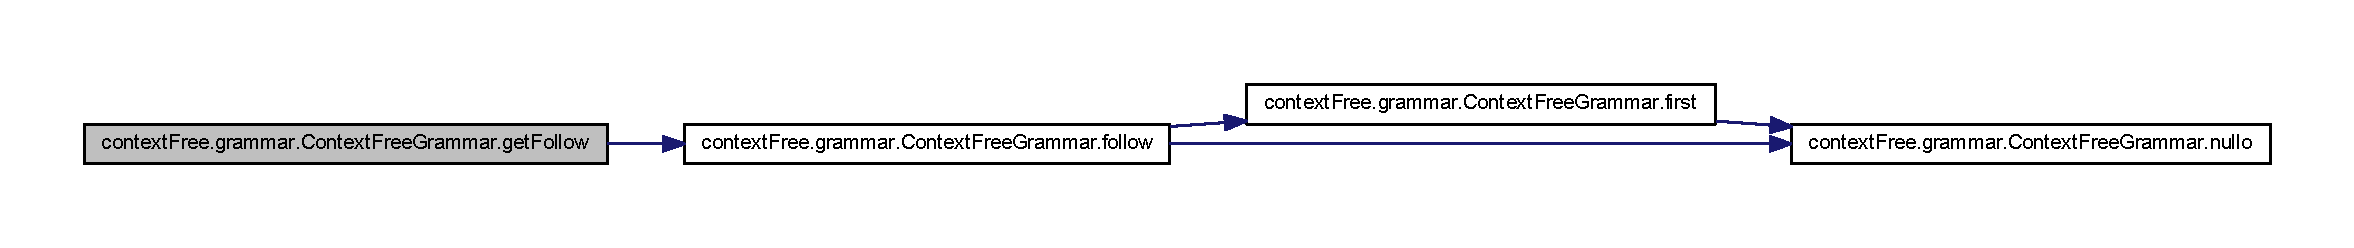
\includegraphics[width=350pt]{classcontext_free_1_1grammar_1_1_context_free_grammar_a5dae0e5de95349d310869fb5941cb5be_cgraph}
\end{center}
\end{figure}


\hypertarget{classcontext_free_1_1grammar_1_1_context_free_grammar_ad00a00b018844cf2acb0c1c5f5d97468}{\index{context\-Free\-::grammar\-::\-Context\-Free\-Grammar@{context\-Free\-::grammar\-::\-Context\-Free\-Grammar}!get\-P@{get\-P}}
\index{get\-P@{get\-P}!contextFree::grammar::ContextFreeGrammar@{context\-Free\-::grammar\-::\-Context\-Free\-Grammar}}
\subsubsection[{get\-P}]{\setlength{\rightskip}{0pt plus 5cm}List$<${\bf Production}$>$ {\bf context\-Free.\-grammar.\-Context\-Free\-Grammar.\-get\-P} (
\begin{DoxyParamCaption}
{}
\end{DoxyParamCaption}
)}}\label{classcontext_free_1_1grammar_1_1_context_free_grammar_ad00a00b018844cf2acb0c1c5f5d97468}


Get production list. 

\begin{DoxyReturn}{Returns}
a list of production objects. 
\end{DoxyReturn}


Implements \hyperlink{interfacecontext_free_1_1grammar_1_1_i_grammar_a629ab4dc36a869b93fa239a3fee760f9}{context\-Free.\-grammar.\-I\-Grammar}.



Definition at line 71 of file Context\-Free\-Grammar.\-java.

\hypertarget{classcontext_free_1_1grammar_1_1_context_free_grammar_ad278c4f5e2bdec1d011d11a3008d8754}{\index{context\-Free\-::grammar\-::\-Context\-Free\-Grammar@{context\-Free\-::grammar\-::\-Context\-Free\-Grammar}!get\-S@{get\-S}}
\index{get\-S@{get\-S}!contextFree::grammar::ContextFreeGrammar@{context\-Free\-::grammar\-::\-Context\-Free\-Grammar}}
\subsubsection[{get\-S}]{\setlength{\rightskip}{0pt plus 5cm}String {\bf context\-Free.\-grammar.\-Context\-Free\-Grammar.\-get\-S} (
\begin{DoxyParamCaption}
{}
\end{DoxyParamCaption}
)}}\label{classcontext_free_1_1grammar_1_1_context_free_grammar_ad278c4f5e2bdec1d011d11a3008d8754}


Get the axioms. 

\begin{DoxyReturn}{Returns}
the axioms 
\end{DoxyReturn}


Implements \hyperlink{interfacecontext_free_1_1grammar_1_1_i_grammar_aceb36e584d26bd39a0f5186742cc9b5b}{context\-Free.\-grammar.\-I\-Grammar}.



Definition at line 81 of file Context\-Free\-Grammar.\-java.

\hypertarget{classcontext_free_1_1grammar_1_1_context_free_grammar_a75f1bbf1e0d1d1350032c628779fcffd}{\index{context\-Free\-::grammar\-::\-Context\-Free\-Grammar@{context\-Free\-::grammar\-::\-Context\-Free\-Grammar}!get\-T@{get\-T}}
\index{get\-T@{get\-T}!contextFree::grammar::ContextFreeGrammar@{context\-Free\-::grammar\-::\-Context\-Free\-Grammar}}
\subsubsection[{get\-T}]{\setlength{\rightskip}{0pt plus 5cm}List$<$String$>$ {\bf context\-Free.\-grammar.\-Context\-Free\-Grammar.\-get\-T} (
\begin{DoxyParamCaption}
{}
\end{DoxyParamCaption}
)}}\label{classcontext_free_1_1grammar_1_1_context_free_grammar_a75f1bbf1e0d1d1350032c628779fcffd}


Get terminal symbols list. 

\begin{DoxyReturn}{Returns}
a list of string with terminal symbol 
\end{DoxyReturn}


Implements \hyperlink{interfacecontext_free_1_1grammar_1_1_i_grammar_a996f5e0bed5a6ac469b764f56d420fb1}{context\-Free.\-grammar.\-I\-Grammar}.



Definition at line 61 of file Context\-Free\-Grammar.\-java.

\hypertarget{classcontext_free_1_1grammar_1_1_context_free_grammar_a664b69a446100c7c4e7a390fb2ee5ebc}{\index{context\-Free\-::grammar\-::\-Context\-Free\-Grammar@{context\-Free\-::grammar\-::\-Context\-Free\-Grammar}!get\-V@{get\-V}}
\index{get\-V@{get\-V}!contextFree::grammar::ContextFreeGrammar@{context\-Free\-::grammar\-::\-Context\-Free\-Grammar}}
\subsubsection[{get\-V}]{\setlength{\rightskip}{0pt plus 5cm}List$<$String$>$ {\bf context\-Free.\-grammar.\-Context\-Free\-Grammar.\-get\-V} (
\begin{DoxyParamCaption}
{}
\end{DoxyParamCaption}
)}}\label{classcontext_free_1_1grammar_1_1_context_free_grammar_a664b69a446100c7c4e7a390fb2ee5ebc}


Get non-\/terminal symbols list. 

\begin{DoxyReturn}{Returns}
a list of string with non-\/terminal symbol 
\end{DoxyReturn}


Implements \hyperlink{interfacecontext_free_1_1grammar_1_1_i_grammar_a4b1bc2134e63051dc37e693294aaeec6}{context\-Free.\-grammar.\-I\-Grammar}.



Definition at line 51 of file Context\-Free\-Grammar.\-java.

\hypertarget{classcontext_free_1_1grammar_1_1_context_free_grammar_ac880ed3ca36ddcd8e20d8279af08244d}{\index{context\-Free\-::grammar\-::\-Context\-Free\-Grammar@{context\-Free\-::grammar\-::\-Context\-Free\-Grammar}!nullo@{nullo}}
\index{nullo@{nullo}!contextFree::grammar::ContextFreeGrammar@{context\-Free\-::grammar\-::\-Context\-Free\-Grammar}}
\subsubsection[{nullo}]{\setlength{\rightskip}{0pt plus 5cm}void context\-Free.\-grammar.\-Context\-Free\-Grammar.\-nullo (
\begin{DoxyParamCaption}
{}
\end{DoxyParamCaption}
)}}\label{classcontext_free_1_1grammar_1_1_context_free_grammar_ac880ed3ca36ddcd8e20d8279af08244d}


population structure Bolean \mbox{[}\mbox{]} null defined in class grammar, it has the same size of V. 

one element is said to null if every component of the expression of the production will be 'null. \begin{DoxyAuthor}{Author}
Pierluigi Sottile 
\end{DoxyAuthor}


Definition at line 121 of file Context\-Free\-Grammar.\-java.



Here is the call graph for this function\-:
\nopagebreak
\begin{figure}[H]
\begin{center}
\leavevmode
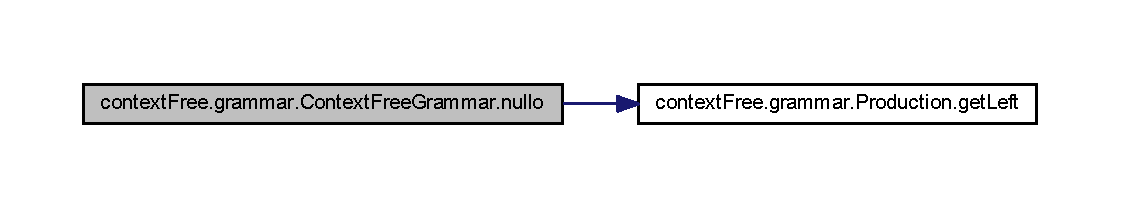
\includegraphics[width=350pt]{classcontext_free_1_1grammar_1_1_context_free_grammar_ac880ed3ca36ddcd8e20d8279af08244d_cgraph}
\end{center}
\end{figure}




Here is the caller graph for this function\-:
\nopagebreak
\begin{figure}[H]
\begin{center}
\leavevmode
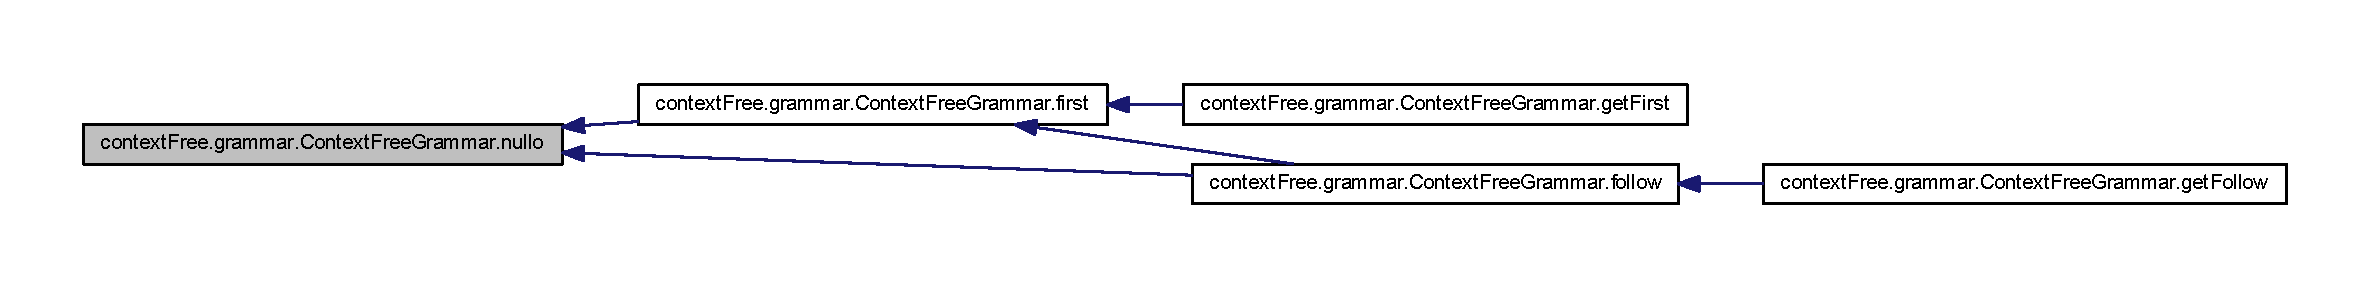
\includegraphics[width=350pt]{classcontext_free_1_1grammar_1_1_context_free_grammar_ac880ed3ca36ddcd8e20d8279af08244d_icgraph}
\end{center}
\end{figure}


\hypertarget{classcontext_free_1_1grammar_1_1_context_free_grammar_a2a66695521702040224c23898b579c92}{\index{context\-Free\-::grammar\-::\-Context\-Free\-Grammar@{context\-Free\-::grammar\-::\-Context\-Free\-Grammar}!set\-P@{set\-P}}
\index{set\-P@{set\-P}!contextFree::grammar::ContextFreeGrammar@{context\-Free\-::grammar\-::\-Context\-Free\-Grammar}}
\subsubsection[{set\-P}]{\setlength{\rightskip}{0pt plus 5cm}void {\bf context\-Free.\-grammar.\-Context\-Free\-Grammar.\-set\-P} (
\begin{DoxyParamCaption}
\item[{List$<$ {\bf Production} $>$}]{p}
\end{DoxyParamCaption}
)}}\label{classcontext_free_1_1grammar_1_1_context_free_grammar_a2a66695521702040224c23898b579c92}


Set the produciton list. 


\begin{DoxyParams}{Parameters}
{\em p} & the list of productions that must be setted. \\
\hline
\end{DoxyParams}


Implements \hyperlink{interfacecontext_free_1_1grammar_1_1_i_grammar_ac070229e5571e47032b5199c0bf2c354}{context\-Free.\-grammar.\-I\-Grammar}.



Definition at line 76 of file Context\-Free\-Grammar.\-java.

\hypertarget{classcontext_free_1_1grammar_1_1_context_free_grammar_a2f4c3ec7270d799ed127cb162e0213b3}{\index{context\-Free\-::grammar\-::\-Context\-Free\-Grammar@{context\-Free\-::grammar\-::\-Context\-Free\-Grammar}!set\-S@{set\-S}}
\index{set\-S@{set\-S}!contextFree::grammar::ContextFreeGrammar@{context\-Free\-::grammar\-::\-Context\-Free\-Grammar}}
\subsubsection[{set\-S}]{\setlength{\rightskip}{0pt plus 5cm}void {\bf context\-Free.\-grammar.\-Context\-Free\-Grammar.\-set\-S} (
\begin{DoxyParamCaption}
\item[{String}]{s}
\end{DoxyParamCaption}
)}}\label{classcontext_free_1_1grammar_1_1_context_free_grammar_a2f4c3ec7270d799ed127cb162e0213b3}


Set the axioms for the grammar. 


\begin{DoxyParams}{Parameters}
{\em s} & the axioms. \\
\hline
\end{DoxyParams}


Implements \hyperlink{interfacecontext_free_1_1grammar_1_1_i_grammar_a134f8b2183ec804eff78ac57b16a0ab9}{context\-Free.\-grammar.\-I\-Grammar}.



Definition at line 86 of file Context\-Free\-Grammar.\-java.

\hypertarget{classcontext_free_1_1grammar_1_1_context_free_grammar_aa1c9a277d660b2ba8443f47cb9543811}{\index{context\-Free\-::grammar\-::\-Context\-Free\-Grammar@{context\-Free\-::grammar\-::\-Context\-Free\-Grammar}!set\-T@{set\-T}}
\index{set\-T@{set\-T}!contextFree::grammar::ContextFreeGrammar@{context\-Free\-::grammar\-::\-Context\-Free\-Grammar}}
\subsubsection[{set\-T}]{\setlength{\rightskip}{0pt plus 5cm}void {\bf context\-Free.\-grammar.\-Context\-Free\-Grammar.\-set\-T} (
\begin{DoxyParamCaption}
\item[{List$<$ String $>$}]{e}
\end{DoxyParamCaption}
)}}\label{classcontext_free_1_1grammar_1_1_context_free_grammar_aa1c9a277d660b2ba8443f47cb9543811}


Set the list of terminal symbols. 


\begin{DoxyParams}{Parameters}
{\em e} & the list of terminal \\
\hline
\end{DoxyParams}


Implements \hyperlink{interfacecontext_free_1_1grammar_1_1_i_grammar_a775125de1388036059da1860ae61a100}{context\-Free.\-grammar.\-I\-Grammar}.



Definition at line 66 of file Context\-Free\-Grammar.\-java.

\hypertarget{classcontext_free_1_1grammar_1_1_context_free_grammar_ad3d3e1efadeb4cc6ed252342fd52c76c}{\index{context\-Free\-::grammar\-::\-Context\-Free\-Grammar@{context\-Free\-::grammar\-::\-Context\-Free\-Grammar}!set\-V@{set\-V}}
\index{set\-V@{set\-V}!contextFree::grammar::ContextFreeGrammar@{context\-Free\-::grammar\-::\-Context\-Free\-Grammar}}
\subsubsection[{set\-V}]{\setlength{\rightskip}{0pt plus 5cm}void {\bf context\-Free.\-grammar.\-Context\-Free\-Grammar.\-set\-V} (
\begin{DoxyParamCaption}
\item[{List$<$ String $>$}]{v}
\end{DoxyParamCaption}
)}}\label{classcontext_free_1_1grammar_1_1_context_free_grammar_ad3d3e1efadeb4cc6ed252342fd52c76c}


Set the list of non-\/terminal symbols. 


\begin{DoxyParams}{Parameters}
{\em v} & the list of non-\/terminal \\
\hline
\end{DoxyParams}


Implements \hyperlink{interfacecontext_free_1_1grammar_1_1_i_grammar_ae7bd17123ad7424af06a7da75a6bc745}{context\-Free.\-grammar.\-I\-Grammar}.



Definition at line 56 of file Context\-Free\-Grammar.\-java.

\hypertarget{classcontext_free_1_1grammar_1_1_context_free_grammar_a922203e2db862d2a8ab31e8e7736273b}{\index{context\-Free\-::grammar\-::\-Context\-Free\-Grammar@{context\-Free\-::grammar\-::\-Context\-Free\-Grammar}!to\-One\-Line\-String@{to\-One\-Line\-String}}
\index{to\-One\-Line\-String@{to\-One\-Line\-String}!contextFree::grammar::ContextFreeGrammar@{context\-Free\-::grammar\-::\-Context\-Free\-Grammar}}
\subsubsection[{to\-One\-Line\-String}]{\setlength{\rightskip}{0pt plus 5cm}String {\bf context\-Free.\-grammar.\-Context\-Free\-Grammar.\-to\-One\-Line\-String} (
\begin{DoxyParamCaption}
{}
\end{DoxyParamCaption}
)}}\label{classcontext_free_1_1grammar_1_1_context_free_grammar_a922203e2db862d2a8ab31e8e7736273b}
\begin{DoxyReturn}{Returns}
the grammar string formatted in one line. 
\end{DoxyReturn}


Implements \hyperlink{interfacecontext_free_1_1grammar_1_1_i_grammar_a5fdeb5a6a9426b400c2fe805566a377c}{context\-Free.\-grammar.\-I\-Grammar}.



Definition at line 337 of file Context\-Free\-Grammar.\-java.



The documentation for this class was generated from the following file\-:\begin{DoxyCompactItemize}
\item 
src/context\-Free/grammar/Context\-Free\-Grammar.\-java\end{DoxyCompactItemize}

\hypertarget{enumerror_1_1_e_r_r_o_r___t_y_p_e}{\section{error.\-E\-R\-R\-O\-R\-\_\-\-T\-Y\-P\-E Enum Reference}
\label{enumerror_1_1_e_r_r_o_r___t_y_p_e}\index{error.\-E\-R\-R\-O\-R\-\_\-\-T\-Y\-P\-E@{error.\-E\-R\-R\-O\-R\-\_\-\-T\-Y\-P\-E}}
}
\subsection*{Public Attributes}
\begin{DoxyCompactItemize}
\item 
\hyperlink{enumerror_1_1_e_r_r_o_r___t_y_p_e_aaf121a60e23c7992ec551d81ebd96f1d}{I\-N\-P\-U\-T\-\_\-\-F\-I\-L\-E}
\item 
\hyperlink{enumerror_1_1_e_r_r_o_r___t_y_p_e_ac6422d34d3c09d323665c858be149f21}{I\-N\-V\-A\-L\-I\-D\-\_\-\-G\-R\-A\-M\-M\-A\-R}
\item 
\hyperlink{enumerror_1_1_e_r_r_o_r___t_y_p_e_a9fa75306960e1fb136a04aa2d4526cf3}{F\-I\-L\-E\-\_\-\-E\-X\-T\-E\-N\-S\-I\-O\-N}
\item 
\hyperlink{enumerror_1_1_e_r_r_o_r___t_y_p_e_a344986e464ffe95c490b7b2278b72d4f}{F\-I\-L\-E\-\_\-\-F\-O\-R\-M\-A\-T}
\item 
\hyperlink{enumerror_1_1_e_r_r_o_r___t_y_p_e_a34b2ee3da4f35c59f641f0eb1e60d06b}{L\-O\-O\-K\-A\-H\-E\-A\-D\-\_\-\-G\-E\-N\-E\-R\-A\-T\-I\-O\-N\-\_\-\-E\-R\-R\-O\-R}
\item 
\hyperlink{enumerror_1_1_e_r_r_o_r___t_y_p_e_a583a3c72741f960e25fb8e45864e40cb}{L\-O\-O\-K\-A\-H\-E\-A\-D\-\_\-\-P\-R\-O\-P\-A\-G\-A\-T\-I\-O\-N\-\_\-\-E\-R\-R\-O\-R}
\item 
\hyperlink{enumerror_1_1_e_r_r_o_r___t_y_p_e_ae438784bc1f218c01def311d198edaaa}{T\-A\-B\-L\-E\-\_\-\-C\-O\-N\-S\-T\-R\-U\-C\-T\-I\-O\-N}
\end{DoxyCompactItemize}


\subsection{Detailed Description}


Definition at line 3 of file E\-R\-R\-O\-R\-\_\-\-T\-Y\-P\-E.\-java.



\subsection{Member Data Documentation}
\hypertarget{enumerror_1_1_e_r_r_o_r___t_y_p_e_a9fa75306960e1fb136a04aa2d4526cf3}{\index{error\-::\-E\-R\-R\-O\-R\-\_\-\-T\-Y\-P\-E@{error\-::\-E\-R\-R\-O\-R\-\_\-\-T\-Y\-P\-E}!F\-I\-L\-E\-\_\-\-E\-X\-T\-E\-N\-S\-I\-O\-N@{F\-I\-L\-E\-\_\-\-E\-X\-T\-E\-N\-S\-I\-O\-N}}
\index{F\-I\-L\-E\-\_\-\-E\-X\-T\-E\-N\-S\-I\-O\-N@{F\-I\-L\-E\-\_\-\-E\-X\-T\-E\-N\-S\-I\-O\-N}!error::ERROR_TYPE@{error\-::\-E\-R\-R\-O\-R\-\_\-\-T\-Y\-P\-E}}
\subsubsection[{F\-I\-L\-E\-\_\-\-E\-X\-T\-E\-N\-S\-I\-O\-N}]{\setlength{\rightskip}{0pt plus 5cm}{\bf error.\-E\-R\-R\-O\-R\-\_\-\-T\-Y\-P\-E.\-F\-I\-L\-E\-\_\-\-E\-X\-T\-E\-N\-S\-I\-O\-N}}}\label{enumerror_1_1_e_r_r_o_r___t_y_p_e_a9fa75306960e1fb136a04aa2d4526cf3}


Definition at line 6 of file E\-R\-R\-O\-R\-\_\-\-T\-Y\-P\-E.\-java.

\hypertarget{enumerror_1_1_e_r_r_o_r___t_y_p_e_a344986e464ffe95c490b7b2278b72d4f}{\index{error\-::\-E\-R\-R\-O\-R\-\_\-\-T\-Y\-P\-E@{error\-::\-E\-R\-R\-O\-R\-\_\-\-T\-Y\-P\-E}!F\-I\-L\-E\-\_\-\-F\-O\-R\-M\-A\-T@{F\-I\-L\-E\-\_\-\-F\-O\-R\-M\-A\-T}}
\index{F\-I\-L\-E\-\_\-\-F\-O\-R\-M\-A\-T@{F\-I\-L\-E\-\_\-\-F\-O\-R\-M\-A\-T}!error::ERROR_TYPE@{error\-::\-E\-R\-R\-O\-R\-\_\-\-T\-Y\-P\-E}}
\subsubsection[{F\-I\-L\-E\-\_\-\-F\-O\-R\-M\-A\-T}]{\setlength{\rightskip}{0pt plus 5cm}{\bf error.\-E\-R\-R\-O\-R\-\_\-\-T\-Y\-P\-E.\-F\-I\-L\-E\-\_\-\-F\-O\-R\-M\-A\-T}}}\label{enumerror_1_1_e_r_r_o_r___t_y_p_e_a344986e464ffe95c490b7b2278b72d4f}


Definition at line 6 of file E\-R\-R\-O\-R\-\_\-\-T\-Y\-P\-E.\-java.

\hypertarget{enumerror_1_1_e_r_r_o_r___t_y_p_e_aaf121a60e23c7992ec551d81ebd96f1d}{\index{error\-::\-E\-R\-R\-O\-R\-\_\-\-T\-Y\-P\-E@{error\-::\-E\-R\-R\-O\-R\-\_\-\-T\-Y\-P\-E}!I\-N\-P\-U\-T\-\_\-\-F\-I\-L\-E@{I\-N\-P\-U\-T\-\_\-\-F\-I\-L\-E}}
\index{I\-N\-P\-U\-T\-\_\-\-F\-I\-L\-E@{I\-N\-P\-U\-T\-\_\-\-F\-I\-L\-E}!error::ERROR_TYPE@{error\-::\-E\-R\-R\-O\-R\-\_\-\-T\-Y\-P\-E}}
\subsubsection[{I\-N\-P\-U\-T\-\_\-\-F\-I\-L\-E}]{\setlength{\rightskip}{0pt plus 5cm}{\bf error.\-E\-R\-R\-O\-R\-\_\-\-T\-Y\-P\-E.\-I\-N\-P\-U\-T\-\_\-\-F\-I\-L\-E}}}\label{enumerror_1_1_e_r_r_o_r___t_y_p_e_aaf121a60e23c7992ec551d81ebd96f1d}


Definition at line 4 of file E\-R\-R\-O\-R\-\_\-\-T\-Y\-P\-E.\-java.

\hypertarget{enumerror_1_1_e_r_r_o_r___t_y_p_e_ac6422d34d3c09d323665c858be149f21}{\index{error\-::\-E\-R\-R\-O\-R\-\_\-\-T\-Y\-P\-E@{error\-::\-E\-R\-R\-O\-R\-\_\-\-T\-Y\-P\-E}!I\-N\-V\-A\-L\-I\-D\-\_\-\-G\-R\-A\-M\-M\-A\-R@{I\-N\-V\-A\-L\-I\-D\-\_\-\-G\-R\-A\-M\-M\-A\-R}}
\index{I\-N\-V\-A\-L\-I\-D\-\_\-\-G\-R\-A\-M\-M\-A\-R@{I\-N\-V\-A\-L\-I\-D\-\_\-\-G\-R\-A\-M\-M\-A\-R}!error::ERROR_TYPE@{error\-::\-E\-R\-R\-O\-R\-\_\-\-T\-Y\-P\-E}}
\subsubsection[{I\-N\-V\-A\-L\-I\-D\-\_\-\-G\-R\-A\-M\-M\-A\-R}]{\setlength{\rightskip}{0pt plus 5cm}{\bf error.\-E\-R\-R\-O\-R\-\_\-\-T\-Y\-P\-E.\-I\-N\-V\-A\-L\-I\-D\-\_\-\-G\-R\-A\-M\-M\-A\-R}}}\label{enumerror_1_1_e_r_r_o_r___t_y_p_e_ac6422d34d3c09d323665c858be149f21}


Definition at line 5 of file E\-R\-R\-O\-R\-\_\-\-T\-Y\-P\-E.\-java.

\hypertarget{enumerror_1_1_e_r_r_o_r___t_y_p_e_a34b2ee3da4f35c59f641f0eb1e60d06b}{\index{error\-::\-E\-R\-R\-O\-R\-\_\-\-T\-Y\-P\-E@{error\-::\-E\-R\-R\-O\-R\-\_\-\-T\-Y\-P\-E}!L\-O\-O\-K\-A\-H\-E\-A\-D\-\_\-\-G\-E\-N\-E\-R\-A\-T\-I\-O\-N\-\_\-\-E\-R\-R\-O\-R@{L\-O\-O\-K\-A\-H\-E\-A\-D\-\_\-\-G\-E\-N\-E\-R\-A\-T\-I\-O\-N\-\_\-\-E\-R\-R\-O\-R}}
\index{L\-O\-O\-K\-A\-H\-E\-A\-D\-\_\-\-G\-E\-N\-E\-R\-A\-T\-I\-O\-N\-\_\-\-E\-R\-R\-O\-R@{L\-O\-O\-K\-A\-H\-E\-A\-D\-\_\-\-G\-E\-N\-E\-R\-A\-T\-I\-O\-N\-\_\-\-E\-R\-R\-O\-R}!error::ERROR_TYPE@{error\-::\-E\-R\-R\-O\-R\-\_\-\-T\-Y\-P\-E}}
\subsubsection[{L\-O\-O\-K\-A\-H\-E\-A\-D\-\_\-\-G\-E\-N\-E\-R\-A\-T\-I\-O\-N\-\_\-\-E\-R\-R\-O\-R}]{\setlength{\rightskip}{0pt plus 5cm}{\bf error.\-E\-R\-R\-O\-R\-\_\-\-T\-Y\-P\-E.\-L\-O\-O\-K\-A\-H\-E\-A\-D\-\_\-\-G\-E\-N\-E\-R\-A\-T\-I\-O\-N\-\_\-\-E\-R\-R\-O\-R}}}\label{enumerror_1_1_e_r_r_o_r___t_y_p_e_a34b2ee3da4f35c59f641f0eb1e60d06b}


Definition at line 7 of file E\-R\-R\-O\-R\-\_\-\-T\-Y\-P\-E.\-java.

\hypertarget{enumerror_1_1_e_r_r_o_r___t_y_p_e_a583a3c72741f960e25fb8e45864e40cb}{\index{error\-::\-E\-R\-R\-O\-R\-\_\-\-T\-Y\-P\-E@{error\-::\-E\-R\-R\-O\-R\-\_\-\-T\-Y\-P\-E}!L\-O\-O\-K\-A\-H\-E\-A\-D\-\_\-\-P\-R\-O\-P\-A\-G\-A\-T\-I\-O\-N\-\_\-\-E\-R\-R\-O\-R@{L\-O\-O\-K\-A\-H\-E\-A\-D\-\_\-\-P\-R\-O\-P\-A\-G\-A\-T\-I\-O\-N\-\_\-\-E\-R\-R\-O\-R}}
\index{L\-O\-O\-K\-A\-H\-E\-A\-D\-\_\-\-P\-R\-O\-P\-A\-G\-A\-T\-I\-O\-N\-\_\-\-E\-R\-R\-O\-R@{L\-O\-O\-K\-A\-H\-E\-A\-D\-\_\-\-P\-R\-O\-P\-A\-G\-A\-T\-I\-O\-N\-\_\-\-E\-R\-R\-O\-R}!error::ERROR_TYPE@{error\-::\-E\-R\-R\-O\-R\-\_\-\-T\-Y\-P\-E}}
\subsubsection[{L\-O\-O\-K\-A\-H\-E\-A\-D\-\_\-\-P\-R\-O\-P\-A\-G\-A\-T\-I\-O\-N\-\_\-\-E\-R\-R\-O\-R}]{\setlength{\rightskip}{0pt plus 5cm}{\bf error.\-E\-R\-R\-O\-R\-\_\-\-T\-Y\-P\-E.\-L\-O\-O\-K\-A\-H\-E\-A\-D\-\_\-\-P\-R\-O\-P\-A\-G\-A\-T\-I\-O\-N\-\_\-\-E\-R\-R\-O\-R}}}\label{enumerror_1_1_e_r_r_o_r___t_y_p_e_a583a3c72741f960e25fb8e45864e40cb}


Definition at line 7 of file E\-R\-R\-O\-R\-\_\-\-T\-Y\-P\-E.\-java.

\hypertarget{enumerror_1_1_e_r_r_o_r___t_y_p_e_ae438784bc1f218c01def311d198edaaa}{\index{error\-::\-E\-R\-R\-O\-R\-\_\-\-T\-Y\-P\-E@{error\-::\-E\-R\-R\-O\-R\-\_\-\-T\-Y\-P\-E}!T\-A\-B\-L\-E\-\_\-\-C\-O\-N\-S\-T\-R\-U\-C\-T\-I\-O\-N@{T\-A\-B\-L\-E\-\_\-\-C\-O\-N\-S\-T\-R\-U\-C\-T\-I\-O\-N}}
\index{T\-A\-B\-L\-E\-\_\-\-C\-O\-N\-S\-T\-R\-U\-C\-T\-I\-O\-N@{T\-A\-B\-L\-E\-\_\-\-C\-O\-N\-S\-T\-R\-U\-C\-T\-I\-O\-N}!error::ERROR_TYPE@{error\-::\-E\-R\-R\-O\-R\-\_\-\-T\-Y\-P\-E}}
\subsubsection[{T\-A\-B\-L\-E\-\_\-\-C\-O\-N\-S\-T\-R\-U\-C\-T\-I\-O\-N}]{\setlength{\rightskip}{0pt plus 5cm}{\bf error.\-E\-R\-R\-O\-R\-\_\-\-T\-Y\-P\-E.\-T\-A\-B\-L\-E\-\_\-\-C\-O\-N\-S\-T\-R\-U\-C\-T\-I\-O\-N}}}\label{enumerror_1_1_e_r_r_o_r___t_y_p_e_ae438784bc1f218c01def311d198edaaa}


Definition at line 7 of file E\-R\-R\-O\-R\-\_\-\-T\-Y\-P\-E.\-java.



The documentation for this enum was generated from the following file\-:\begin{DoxyCompactItemize}
\item 
src/error/\hyperlink{_e_r_r_o_r___t_y_p_e_8java}{E\-R\-R\-O\-R\-\_\-\-T\-Y\-P\-E.\-java}\end{DoxyCompactItemize}

\hypertarget{classerror_1_1_error_manager}{\section{error.\-Error\-Manager Class Reference}
\label{classerror_1_1_error_manager}\index{error.\-Error\-Manager@{error.\-Error\-Manager}}
}


Collaboration diagram for error.\-Error\-Manager\-:\nopagebreak
\begin{figure}[H]
\begin{center}
\leavevmode
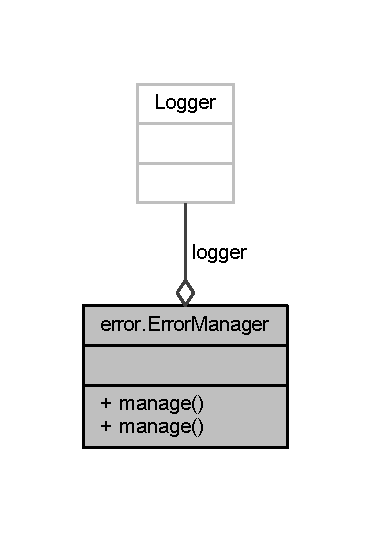
\includegraphics[width=178pt]{classerror_1_1_error_manager__coll__graph}
\end{center}
\end{figure}
\subsection*{Static Public Member Functions}
\begin{DoxyCompactItemize}
\item 
\hypertarget{classerror_1_1_error_manager_a22faa52ee5734184fa446591fd45ba7f}{static void {\bfseries manage} (\hyperlink{enumerror_1_1_e_r_r_o_r___t_y_p_e}{E\-R\-R\-O\-R\-\_\-\-T\-Y\-P\-E} type)}\label{classerror_1_1_error_manager_a22faa52ee5734184fa446591fd45ba7f}

\item 
\hypertarget{classerror_1_1_error_manager_aa17e91fab94fd42d865e53eaec80e2cb}{static void {\bfseries manage} (\hyperlink{enumerror_1_1_e_r_r_o_r___t_y_p_e}{E\-R\-R\-O\-R\-\_\-\-T\-Y\-P\-E} type, Exception e)  throws Exception}\label{classerror_1_1_error_manager_aa17e91fab94fd42d865e53eaec80e2cb}

\end{DoxyCompactItemize}
\subsection*{Static Package Attributes}
\begin{DoxyCompactItemize}
\item 
\hypertarget{classerror_1_1_error_manager_abf11a50b38703340894a680bd8230144}{static Logger {\bfseries logger} = Logger.\-get\-Logger(Error\-Manager.\-class.\-get\-Name())}\label{classerror_1_1_error_manager_abf11a50b38703340894a680bd8230144}

\end{DoxyCompactItemize}


\subsection{Detailed Description}


Definition at line 6 of file Error\-Manager.\-java.



The documentation for this class was generated from the following file\-:\begin{DoxyCompactItemize}
\item 
src/error/Error\-Manager.\-java\end{DoxyCompactItemize}

\hypertarget{class_file_chooser}{\section{File\-Chooser Class Reference}
\label{class_file_chooser}\index{File\-Chooser@{File\-Chooser}}
}
\subsection*{Static Private Attributes}
\begin{DoxyCompactItemize}
\item 
\hypertarget{class_file_chooser_a3cbd18488adfa238990fc2faf44a2931}{static final long {\bfseries serial\-Version\-U\-I\-D} = 1\-L}\label{class_file_chooser_a3cbd18488adfa238990fc2faf44a2931}

\end{DoxyCompactItemize}


\subsection{Detailed Description}
\begin{DoxyAuthor}{Author}
Paolo Pino 
\end{DoxyAuthor}


Definition at line 8 of file File\-Chooser.\-java.



The documentation for this class was generated from the following file\-:\begin{DoxyCompactItemize}
\item 
src/File\-Chooser.\-java\end{DoxyCompactItemize}

\hypertarget{classinput_parser_1_1_four_line_input_parser}{\section{input\-Parser.\-Four\-Line\-Input\-Parser Class Reference}
\label{classinput_parser_1_1_four_line_input_parser}\index{input\-Parser.\-Four\-Line\-Input\-Parser@{input\-Parser.\-Four\-Line\-Input\-Parser}}
}


Parse a four line grammar format.  




Inheritance diagram for input\-Parser.\-Four\-Line\-Input\-Parser\-:\nopagebreak
\begin{figure}[H]
\begin{center}
\leavevmode
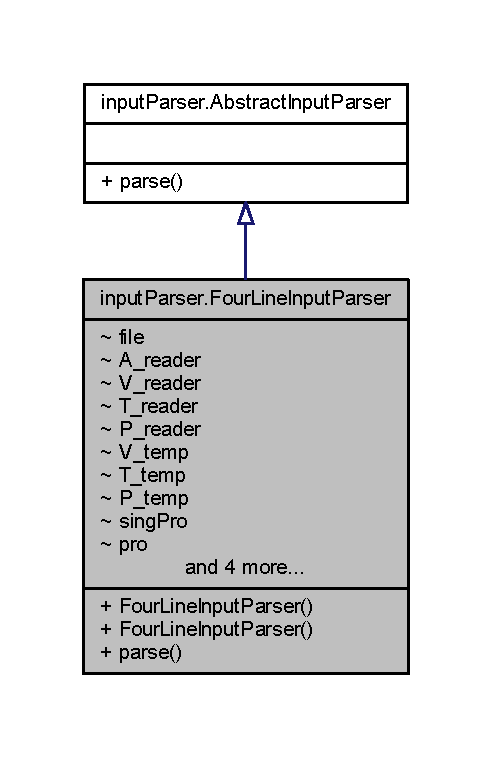
\includegraphics[width=236pt]{classinput_parser_1_1_four_line_input_parser__inherit__graph}
\end{center}
\end{figure}


Collaboration diagram for input\-Parser.\-Four\-Line\-Input\-Parser\-:\nopagebreak
\begin{figure}[H]
\begin{center}
\leavevmode
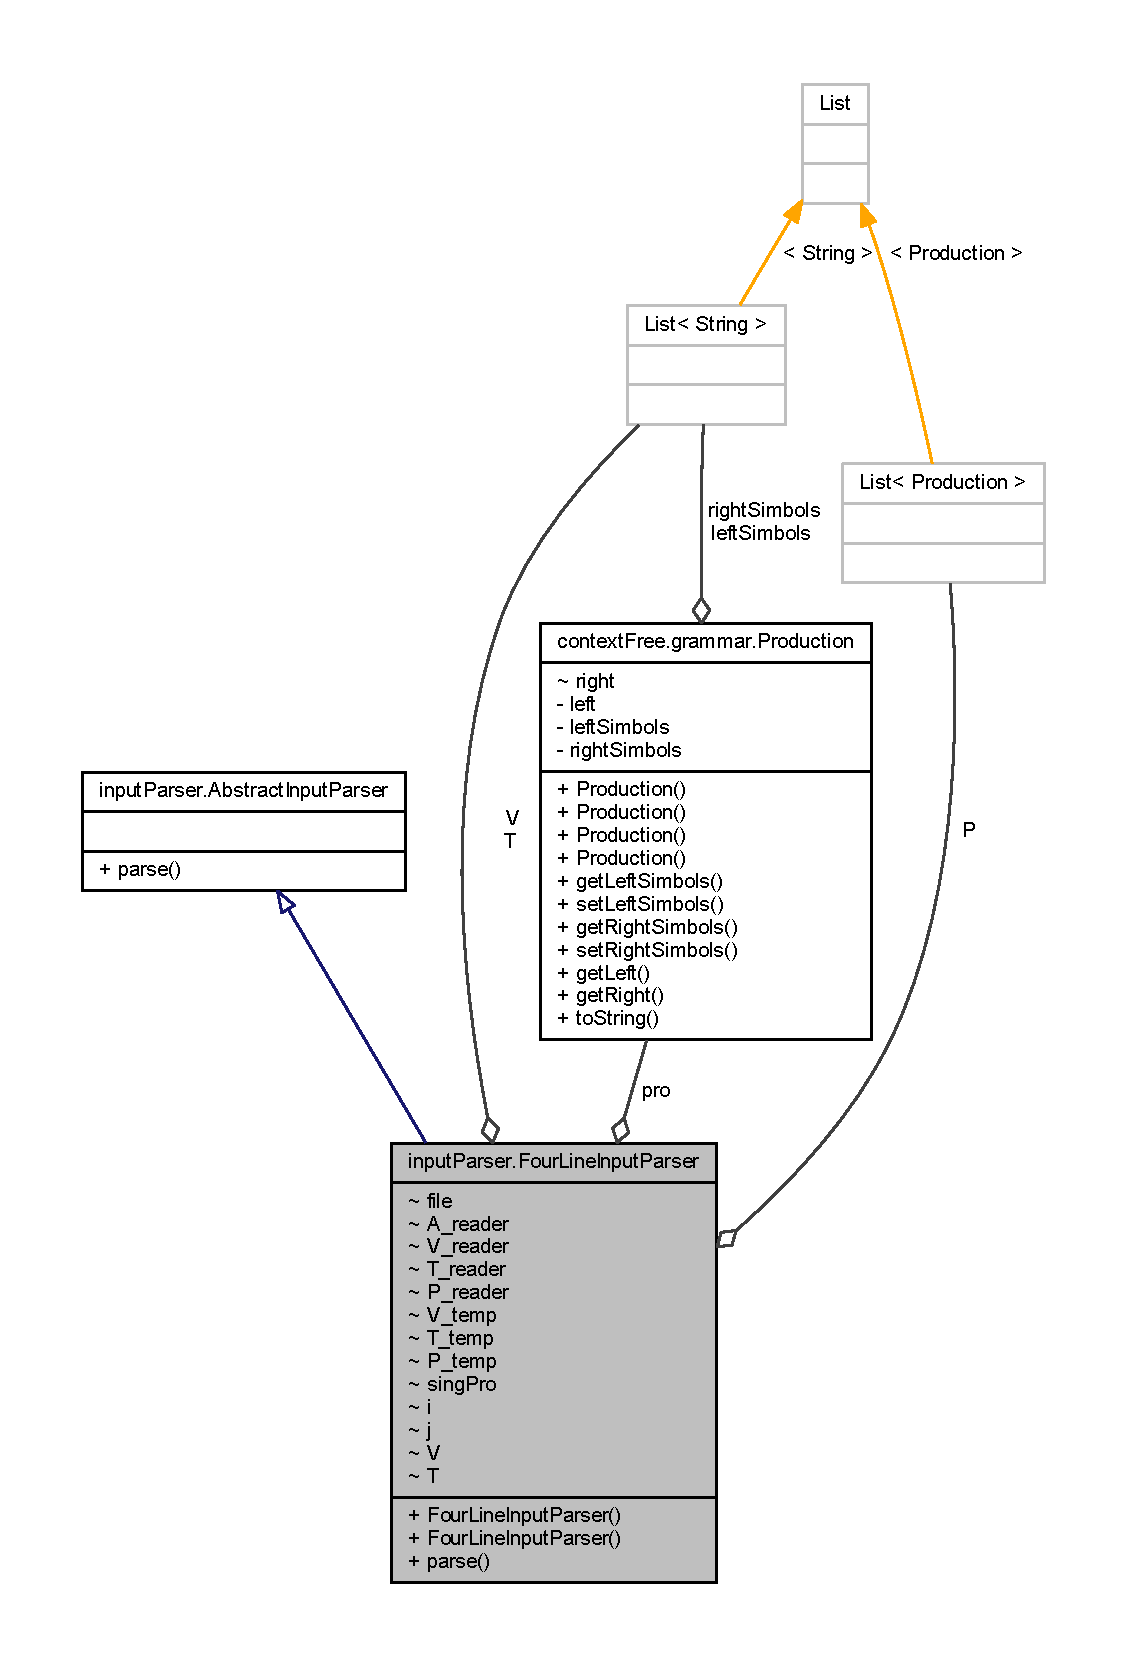
\includegraphics[width=350pt]{classinput_parser_1_1_four_line_input_parser__coll__graph}
\end{center}
\end{figure}
\subsection*{Public Member Functions}
\begin{DoxyCompactItemize}
\item 
\hypertarget{classinput_parser_1_1_four_line_input_parser_ab60c07b777f5edc493d0d71abcfdc840}{{\bfseries Four\-Line\-Input\-Parser} (String input)}\label{classinput_parser_1_1_four_line_input_parser_ab60c07b777f5edc493d0d71abcfdc840}

\item 
\hyperlink{interfacecontext_free_1_1grammar_1_1_i_grammar}{I\-Grammar} \hyperlink{classinput_parser_1_1_four_line_input_parser_a99c37488d66cfeecb33e13d573b4a81a}{parse} ()  throws Exception
\begin{DoxyCompactList}\small\item\em Read the file .4l and creates the object grammar. \end{DoxyCompactList}\end{DoxyCompactItemize}
\subsection*{Package Attributes}
\begin{DoxyCompactItemize}
\item 
\hypertarget{classinput_parser_1_1_four_line_input_parser_ab974828c70b8a1335c806d6d3cf83da7}{String {\bfseries file}}\label{classinput_parser_1_1_four_line_input_parser_ab974828c70b8a1335c806d6d3cf83da7}

\item 
\hypertarget{classinput_parser_1_1_four_line_input_parser_a9ed7517e786d914194ee6e2e7a2dedf9}{String {\bfseries A\-\_\-reader}}\label{classinput_parser_1_1_four_line_input_parser_a9ed7517e786d914194ee6e2e7a2dedf9}

\item 
\hypertarget{classinput_parser_1_1_four_line_input_parser_ab32a6cf6e1398b4d6df4cde2036dfc82}{String {\bfseries V\-\_\-reader}}\label{classinput_parser_1_1_four_line_input_parser_ab32a6cf6e1398b4d6df4cde2036dfc82}

\item 
\hypertarget{classinput_parser_1_1_four_line_input_parser_ac942629b7fbdf58ea902eaccfba356b4}{String {\bfseries T\-\_\-reader}}\label{classinput_parser_1_1_four_line_input_parser_ac942629b7fbdf58ea902eaccfba356b4}

\item 
\hypertarget{classinput_parser_1_1_four_line_input_parser_a72862efdd54896c843b7ad5677f33515}{String {\bfseries P\-\_\-reader}}\label{classinput_parser_1_1_four_line_input_parser_a72862efdd54896c843b7ad5677f33515}

\item 
\hypertarget{classinput_parser_1_1_four_line_input_parser_a70d648d67b885eeef32f47162ffa81ae}{String\mbox{[}$\,$\mbox{]} {\bfseries V\-\_\-temp}}\label{classinput_parser_1_1_four_line_input_parser_a70d648d67b885eeef32f47162ffa81ae}

\item 
\hypertarget{classinput_parser_1_1_four_line_input_parser_a17b5ddecc36fdca0cc0be1d613a20caa}{String\mbox{[}$\,$\mbox{]} {\bfseries T\-\_\-temp}}\label{classinput_parser_1_1_four_line_input_parser_a17b5ddecc36fdca0cc0be1d613a20caa}

\item 
\hypertarget{classinput_parser_1_1_four_line_input_parser_adb2b6b325e8bc451ba7b46270ba4dea8}{String\mbox{[}$\,$\mbox{]} {\bfseries P\-\_\-temp}}\label{classinput_parser_1_1_four_line_input_parser_adb2b6b325e8bc451ba7b46270ba4dea8}

\item 
\hypertarget{classinput_parser_1_1_four_line_input_parser_a7a3bb0e55f839ba984d0953724ea385a}{String\mbox{[}$\,$\mbox{]} {\bfseries sing\-Pro}}\label{classinput_parser_1_1_four_line_input_parser_a7a3bb0e55f839ba984d0953724ea385a}

\item 
\hypertarget{classinput_parser_1_1_four_line_input_parser_ae0f524894f39d7a13bddd5e2efad8d3e}{\hyperlink{classcontext_free_1_1grammar_1_1_production}{Production} {\bfseries pro}}\label{classinput_parser_1_1_four_line_input_parser_ae0f524894f39d7a13bddd5e2efad8d3e}

\item 
\hypertarget{classinput_parser_1_1_four_line_input_parser_a39fe356d1b2152557ca7c5d47b0d2f43}{int {\bfseries i}}\label{classinput_parser_1_1_four_line_input_parser_a39fe356d1b2152557ca7c5d47b0d2f43}

\item 
\hypertarget{classinput_parser_1_1_four_line_input_parser_a6aaf88a0bec2622e542a59b4efdd19b6}{int {\bfseries j}}\label{classinput_parser_1_1_four_line_input_parser_a6aaf88a0bec2622e542a59b4efdd19b6}

\item 
\hypertarget{classinput_parser_1_1_four_line_input_parser_a1dd8814f232e9c83f48ead8cf5d9f2b2}{List$<$ String $>$ {\bfseries V} = null}\label{classinput_parser_1_1_four_line_input_parser_a1dd8814f232e9c83f48ead8cf5d9f2b2}

\item 
\hypertarget{classinput_parser_1_1_four_line_input_parser_ac5810e00377c73d3218c6c517676c5d4}{List$<$ String $>$ {\bfseries T} = null}\label{classinput_parser_1_1_four_line_input_parser_ac5810e00377c73d3218c6c517676c5d4}

\item 
\hypertarget{classinput_parser_1_1_four_line_input_parser_a25cb1cc11bda9a906f0a29eb66444c76}{List$<$ \hyperlink{classcontext_free_1_1grammar_1_1_production}{Production} $>$ {\bfseries P} = null}\label{classinput_parser_1_1_four_line_input_parser_a25cb1cc11bda9a906f0a29eb66444c76}

\end{DoxyCompactItemize}


\subsection{Detailed Description}
Parse a four line grammar format. 

ex (file.\-4l)\-: E E, T, P a, +, x, (, ), \$ E\-:\-:=E+\-T, E\-:\-:=T, T\-:\-:=Tx\-P, T\-:\-:=P, P\-:\-:=a, P\-:\-:=(E) \begin{DoxyAuthor}{Author}
Pierluigi Sottile 
\end{DoxyAuthor}


Definition at line 26 of file Four\-Line\-Input\-Parser.\-java.



\subsection{Member Function Documentation}
\hypertarget{classinput_parser_1_1_four_line_input_parser_a99c37488d66cfeecb33e13d573b4a81a}{\index{input\-Parser\-::\-Four\-Line\-Input\-Parser@{input\-Parser\-::\-Four\-Line\-Input\-Parser}!parse@{parse}}
\index{parse@{parse}!inputParser::FourLineInputParser@{input\-Parser\-::\-Four\-Line\-Input\-Parser}}
\subsubsection[{parse}]{\setlength{\rightskip}{0pt plus 5cm}{\bf I\-Grammar} {\bf input\-Parser.\-Four\-Line\-Input\-Parser.\-parse} (
\begin{DoxyParamCaption}
{}
\end{DoxyParamCaption}
)  throws Exception\hspace{0.3cm}{\ttfamily  \mbox{[}virtual\mbox{]}}}}\label{classinput_parser_1_1_four_line_input_parser_a99c37488d66cfeecb33e13d573b4a81a}


Read the file .4l and creates the object grammar. 

\begin{DoxyReturn}{Returns}
the grammar 
\end{DoxyReturn}
\begin{DoxyAuthor}{Author}
Pierluigi Sottile 
\end{DoxyAuthor}


Implements \hyperlink{classinput_parser_1_1_abstract_input_parser_a548b0f6fa44b7954b79bdd964336bafe}{input\-Parser.\-Abstract\-Input\-Parser}.



Definition at line 54 of file Four\-Line\-Input\-Parser.\-java.



Here is the call graph for this function\-:\nopagebreak
\begin{figure}[H]
\begin{center}
\leavevmode
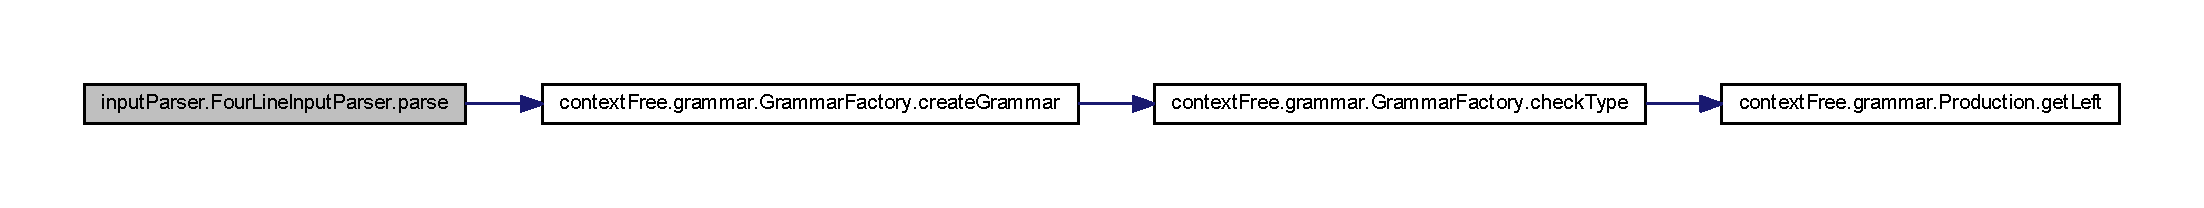
\includegraphics[width=350pt]{classinput_parser_1_1_four_line_input_parser_a99c37488d66cfeecb33e13d573b4a81a_cgraph}
\end{center}
\end{figure}




The documentation for this class was generated from the following file\-:\begin{DoxyCompactItemize}
\item 
src/input\-Parser/Four\-Line\-Input\-Parser.\-java\end{DoxyCompactItemize}

\hypertarget{class_generic_file_filter}{\section{Generic\-File\-Filter Class Reference}
\label{class_generic_file_filter}\index{Generic\-File\-Filter@{Generic\-File\-Filter}}
}


Filter the file type for the file chooser.  




Inheritance diagram for Generic\-File\-Filter\-:
\nopagebreak
\begin{figure}[H]
\begin{center}
\leavevmode
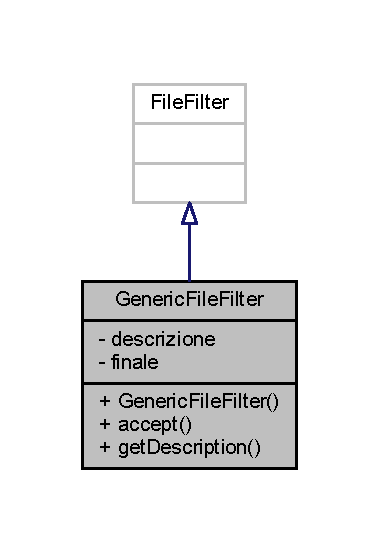
\includegraphics[width=182pt]{class_generic_file_filter__inherit__graph}
\end{center}
\end{figure}


Collaboration diagram for Generic\-File\-Filter\-:
\nopagebreak
\begin{figure}[H]
\begin{center}
\leavevmode
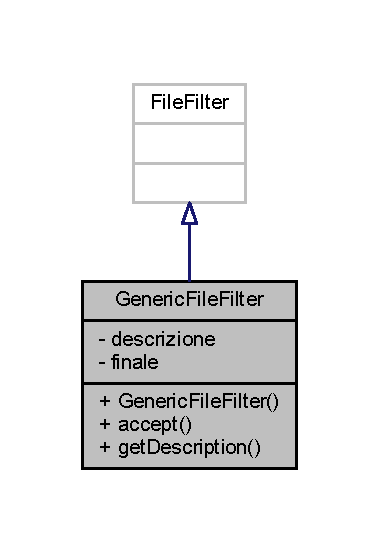
\includegraphics[width=182pt]{class_generic_file_filter__coll__graph}
\end{center}
\end{figure}
\subsection*{Public Member Functions}
\begin{DoxyCompactItemize}
\item 
\hypertarget{class_generic_file_filter_a96d78c6c212bfbf0be95a4d10937a89d}{{\bfseries Generic\-File\-Filter} (String descrizione, String estensione)}\label{class_generic_file_filter_a96d78c6c212bfbf0be95a4d10937a89d}

\item 
\hypertarget{class_generic_file_filter_a03eee4e0d87525559746265dc63c9319}{boolean {\bfseries accept} (File f)}\label{class_generic_file_filter_a03eee4e0d87525559746265dc63c9319}

\item 
\hypertarget{class_generic_file_filter_a6918acbc60f5dcff51cb92a9487e2493}{String {\bfseries get\-Description} ()}\label{class_generic_file_filter_a6918acbc60f5dcff51cb92a9487e2493}

\end{DoxyCompactItemize}
\subsection*{Private Attributes}
\begin{DoxyCompactItemize}
\item 
\hypertarget{class_generic_file_filter_a9953e3b3aa3dee91452cb9c2ad80822b}{String {\bfseries descrizione}}\label{class_generic_file_filter_a9953e3b3aa3dee91452cb9c2ad80822b}

\item 
\hypertarget{class_generic_file_filter_a9468f04e6ea80d41e6bc69b59769b751}{String {\bfseries finale}}\label{class_generic_file_filter_a9468f04e6ea80d41e6bc69b59769b751}

\end{DoxyCompactItemize}


\subsection{Detailed Description}
Filter the file type for the file chooser. 

\begin{DoxyAuthor}{Author}
Paolo Pino 
\end{DoxyAuthor}


Definition at line 10 of file Generic\-File\-Filter.\-java.



The documentation for this class was generated from the following file\-:\begin{DoxyCompactItemize}
\item 
src/Generic\-File\-Filter.\-java\end{DoxyCompactItemize}

\hypertarget{enumcontext_free_1_1grammar_1_1_g_r_a_m_m_a_r___t_y_p_e}{\section{context\-Free.\-grammar.\-G\-R\-A\-M\-M\-A\-R\-\_\-\-T\-Y\-P\-E Enum Reference}
\label{enumcontext_free_1_1grammar_1_1_g_r_a_m_m_a_r___t_y_p_e}\index{context\-Free.\-grammar.\-G\-R\-A\-M\-M\-A\-R\-\_\-\-T\-Y\-P\-E@{context\-Free.\-grammar.\-G\-R\-A\-M\-M\-A\-R\-\_\-\-T\-Y\-P\-E}}
}


Specify the type of a grammar.  


\subsection*{Public Attributes}
\begin{DoxyCompactItemize}
\item 
\hypertarget{enumcontext_free_1_1grammar_1_1_g_r_a_m_m_a_r___t_y_p_e_a1716ccff248a4c662919f646073266e2}{{\bfseries C\-O\-N\-T\-E\-X\-T\-\_\-\-F\-R\-E\-E}}\label{enumcontext_free_1_1grammar_1_1_g_r_a_m_m_a_r___t_y_p_e_a1716ccff248a4c662919f646073266e2}

\end{DoxyCompactItemize}


\subsection{Detailed Description}
Specify the type of a grammar. 

\begin{DoxyAuthor}{Author}
Paolo Pino 
\end{DoxyAuthor}


Definition at line 7 of file G\-R\-A\-M\-M\-A\-R\-\_\-\-T\-Y\-P\-E.\-java.



The documentation for this enum was generated from the following file\-:\begin{DoxyCompactItemize}
\item 
src/context\-Free/grammar/G\-R\-A\-M\-M\-A\-R\-\_\-\-T\-Y\-P\-E.\-java\end{DoxyCompactItemize}

\hypertarget{classcontext_free_1_1grammar_1_1_grammar_factory}{\section{context\-Free.\-grammar.\-Grammar\-Factory Class Reference}
\label{classcontext_free_1_1grammar_1_1_grammar_factory}\index{context\-Free.\-grammar.\-Grammar\-Factory@{context\-Free.\-grammar.\-Grammar\-Factory}}
}
\subsection*{Static Public Member Functions}
\begin{DoxyCompactItemize}
\item 
static \hyperlink{interfacecontext_free_1_1grammar_1_1_i_grammar}{I\-Grammar} \hyperlink{classcontext_free_1_1grammar_1_1_grammar_factory_a6829a8d168584b20ac594fae87de591a}{create\-Context\-Free\-Grammar} (String ass, List$<$ \hyperlink{classcontext_free_1_1grammar_1_1_production}{Production} $>$ prod)
\item 
static \hyperlink{interfacecontext_free_1_1grammar_1_1_i_grammar}{I\-Grammar} \hyperlink{classcontext_free_1_1grammar_1_1_grammar_factory_a25d4e5bf4a9a452efca5dd6518e16c25}{create\-Grammar} (String ass, List$<$ \hyperlink{classcontext_free_1_1grammar_1_1_production}{Production} $>$ prod, List$<$ String $>$ V, List$<$ String $>$ T)
\begin{DoxyCompactList}\small\item\em Check the type of grammar (eg Contex-\/free) and returns the correct instance. \end{DoxyCompactList}\end{DoxyCompactItemize}
\subsection*{Static Private Member Functions}
\begin{DoxyCompactItemize}
\item 
static \hyperlink{enumcontext_free_1_1grammar_1_1_g_r_a_m_m_a_r___t_y_p_e}{G\-R\-A\-M\-M\-A\-R\-\_\-\-T\-Y\-P\-E} \hyperlink{classcontext_free_1_1grammar_1_1_grammar_factory_a513482168bb15e55211bc4f04e276711}{check\-Type} (List$<$ \hyperlink{classcontext_free_1_1grammar_1_1_production}{Production} $>$ prod, List$<$ String $>$ V, List$<$ String $>$ T)
\begin{DoxyCompactList}\small\item\em controls that make up the grammar productions that are valid \end{DoxyCompactList}\end{DoxyCompactItemize}


\subsection{Detailed Description}


Definition at line 7 of file Grammar\-Factory.\-java.



\subsection{Member Function Documentation}
\hypertarget{classcontext_free_1_1grammar_1_1_grammar_factory_a513482168bb15e55211bc4f04e276711}{\index{context\-Free\-::grammar\-::\-Grammar\-Factory@{context\-Free\-::grammar\-::\-Grammar\-Factory}!check\-Type@{check\-Type}}
\index{check\-Type@{check\-Type}!contextFree::grammar::GrammarFactory@{context\-Free\-::grammar\-::\-Grammar\-Factory}}
\subsubsection[{check\-Type}]{\setlength{\rightskip}{0pt plus 5cm}static {\bf G\-R\-A\-M\-M\-A\-R\-\_\-\-T\-Y\-P\-E} {\bf context\-Free.\-grammar.\-Grammar\-Factory.\-check\-Type} (
\begin{DoxyParamCaption}
\item[{List$<$ {\bf Production} $>$}]{prod, }
\item[{List$<$ String $>$}]{V, }
\item[{List$<$ String $>$}]{T}
\end{DoxyParamCaption}
)\hspace{0.3cm}{\ttfamily  \mbox{[}static, private\mbox{]}}}}\label{classcontext_free_1_1grammar_1_1_grammar_factory_a513482168bb15e55211bc4f04e276711}


controls that make up the grammar productions that are valid 


\begin{DoxyParams}{Parameters}
{\em List} & of prodaction \\
\hline
{\em list} & of Not-\/terminal simbol \\
\hline
{\em list} & of Terminal Simbol \\
\hline
\end{DoxyParams}
\begin{DoxyReturn}{Returns}

\end{DoxyReturn}
\begin{DoxyAuthor}{Author}
Pierluigi Sottile 
\end{DoxyAuthor}


Definition at line 40 of file Grammar\-Factory.\-java.

\hypertarget{classcontext_free_1_1grammar_1_1_grammar_factory_a6829a8d168584b20ac594fae87de591a}{\index{context\-Free\-::grammar\-::\-Grammar\-Factory@{context\-Free\-::grammar\-::\-Grammar\-Factory}!create\-Context\-Free\-Grammar@{create\-Context\-Free\-Grammar}}
\index{create\-Context\-Free\-Grammar@{create\-Context\-Free\-Grammar}!contextFree::grammar::GrammarFactory@{context\-Free\-::grammar\-::\-Grammar\-Factory}}
\subsubsection[{create\-Context\-Free\-Grammar}]{\setlength{\rightskip}{0pt plus 5cm}static {\bf I\-Grammar} {\bf context\-Free.\-grammar.\-Grammar\-Factory.\-create\-Context\-Free\-Grammar} (
\begin{DoxyParamCaption}
\item[{String}]{ass, }
\item[{List$<$ {\bf Production} $>$}]{prod}
\end{DoxyParamCaption}
)\hspace{0.3cm}{\ttfamily  \mbox{[}static\mbox{]}}}}\label{classcontext_free_1_1grammar_1_1_grammar_factory_a6829a8d168584b20ac594fae87de591a}


Definition at line 8 of file Grammar\-Factory.\-java.

\hypertarget{classcontext_free_1_1grammar_1_1_grammar_factory_a25d4e5bf4a9a452efca5dd6518e16c25}{\index{context\-Free\-::grammar\-::\-Grammar\-Factory@{context\-Free\-::grammar\-::\-Grammar\-Factory}!create\-Grammar@{create\-Grammar}}
\index{create\-Grammar@{create\-Grammar}!contextFree::grammar::GrammarFactory@{context\-Free\-::grammar\-::\-Grammar\-Factory}}
\subsubsection[{create\-Grammar}]{\setlength{\rightskip}{0pt plus 5cm}static {\bf I\-Grammar} {\bf context\-Free.\-grammar.\-Grammar\-Factory.\-create\-Grammar} (
\begin{DoxyParamCaption}
\item[{String}]{ass, }
\item[{List$<$ {\bf Production} $>$}]{prod, }
\item[{List$<$ String $>$}]{V, }
\item[{List$<$ String $>$}]{T}
\end{DoxyParamCaption}
)\hspace{0.3cm}{\ttfamily  \mbox{[}static\mbox{]}}}}\label{classcontext_free_1_1grammar_1_1_grammar_factory_a25d4e5bf4a9a452efca5dd6518e16c25}


Check the type of grammar (eg Contex-\/free) and returns the correct instance. 


\begin{DoxyParams}{Parameters}
{\em Assioma} & \\
\hline
{\em List} & of Prodaction \\
\hline
{\em List} & of Not Termianl Simbol \\
\hline
{\em list} & of Termianl Simbol \\
\hline
\end{DoxyParams}
\begin{DoxyReturn}{Returns}

\end{DoxyReturn}
\begin{DoxyAuthor}{Author}
Pierluigi Sottile 
\end{DoxyAuthor}


Definition at line 21 of file Grammar\-Factory.\-java.



The documentation for this class was generated from the following file\-:\begin{DoxyCompactItemize}
\item 
src/context\-Free/grammar/\hyperlink{_grammar_factory_8java}{Grammar\-Factory.\-java}\end{DoxyCompactItemize}

\hypertarget{classparser_program_1_1_history_element}{\section{parser\-Program.\-History\-Element Class Reference}
\label{classparser_program_1_1_history_element}\index{parser\-Program.\-History\-Element@{parser\-Program.\-History\-Element}}
}


This class represent an element of the parsing history.  




Collaboration diagram for parser\-Program.\-History\-Element\-:\nopagebreak
\begin{figure}[H]
\begin{center}
\leavevmode
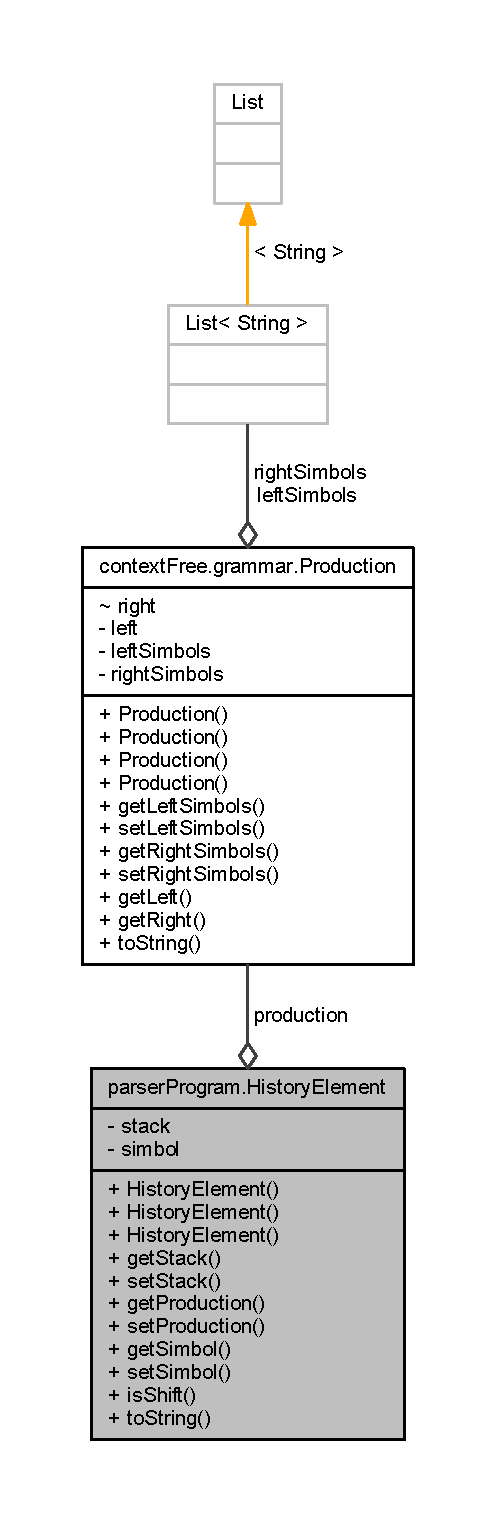
\includegraphics[height=550pt]{classparser_program_1_1_history_element__coll__graph}
\end{center}
\end{figure}
\subsection*{Public Member Functions}
\begin{DoxyCompactItemize}
\item 
\hypertarget{classparser_program_1_1_history_element_a45f360f314f688585844a62592bdb5c5}{\hyperlink{classparser_program_1_1_history_element_a45f360f314f688585844a62592bdb5c5}{History\-Element} ()}\label{classparser_program_1_1_history_element_a45f360f314f688585844a62592bdb5c5}

\begin{DoxyCompactList}\small\item\em Default constructor. \end{DoxyCompactList}\item 
\hyperlink{classparser_program_1_1_history_element_ae6d3bdd3606301f0b08d4e9258b5c5cf}{History\-Element} (String\mbox{[}$\,$\mbox{]} stk)
\begin{DoxyCompactList}\small\item\em Construct the object with specified parsing stack. \end{DoxyCompactList}\item 
\hyperlink{classparser_program_1_1_history_element_a0cd8852d35a48856c6e893ae33cbde30}{History\-Element} (String\mbox{[}$\,$\mbox{]} stk, \hyperlink{classcontext_free_1_1grammar_1_1_production}{Production} p, String s)
\begin{DoxyCompactList}\small\item\em Construct the object with specified parsing stack, production and step. \end{DoxyCompactList}\item 
String\mbox{[}$\,$\mbox{]} \hyperlink{classparser_program_1_1_history_element_a8f20a699af1fa68f114acef0f72117b5}{get\-Stack} ()
\item 
void \hyperlink{classparser_program_1_1_history_element_a640ecb265a57f1b084fe99cf2a2a9a35}{set\-Stack} (String\mbox{[}$\,$\mbox{]} stack)
\begin{DoxyCompactList}\small\item\em Set the stack. \end{DoxyCompactList}\item 
\hyperlink{classcontext_free_1_1grammar_1_1_production}{Production} \hyperlink{classparser_program_1_1_history_element_a1e3354d1bc805c952c4ed9a35ddac0dd}{get\-Production} ()
\item 
void \hyperlink{classparser_program_1_1_history_element_a2311f48be369f4d0e6be47c2a7ac7546}{set\-Production} (\hyperlink{classcontext_free_1_1grammar_1_1_production}{Production} production)
\begin{DoxyCompactList}\small\item\em Set the production. \end{DoxyCompactList}\item 
String \hyperlink{classparser_program_1_1_history_element_ab64610fe65f58bca7d542244378ac030}{get\-Simbol} ()
\item 
void \hyperlink{classparser_program_1_1_history_element_a54ecd254d7abd49d0d10230892dfc35b}{set\-Simbol} (String simbol)
\begin{DoxyCompactList}\small\item\em Set the parsing step. \end{DoxyCompactList}\item 
boolean \hyperlink{classparser_program_1_1_history_element_a233c9c55643f4d6bc8103c4e2c8bd038}{is\-Shift} ()
\item 
\hypertarget{classparser_program_1_1_history_element_aa0ddd25dd8d27e59d63123b2f50e1cb4}{String {\bfseries to\-String} ()}\label{classparser_program_1_1_history_element_aa0ddd25dd8d27e59d63123b2f50e1cb4}

\end{DoxyCompactItemize}
\subsection*{Private Attributes}
\begin{DoxyCompactItemize}
\item 
\hypertarget{classparser_program_1_1_history_element_a3ab04c9be50cda70dcfd9ee134884d9f}{String\mbox{[}$\,$\mbox{]} {\bfseries stack}}\label{classparser_program_1_1_history_element_a3ab04c9be50cda70dcfd9ee134884d9f}

\item 
\hypertarget{classparser_program_1_1_history_element_a93323e030ba302f08564c7d6cd021a15}{\hyperlink{classcontext_free_1_1grammar_1_1_production}{Production} {\bfseries production}}\label{classparser_program_1_1_history_element_a93323e030ba302f08564c7d6cd021a15}

\item 
\hypertarget{classparser_program_1_1_history_element_a3c9ad24a6a0f33ac5d1cbc95ff1e82de}{String {\bfseries simbol}}\label{classparser_program_1_1_history_element_a3c9ad24a6a0f33ac5d1cbc95ff1e82de}

\end{DoxyCompactItemize}


\subsection{Detailed Description}
This class represent an element of the parsing history. 

\begin{DoxyAuthor}{Author}
Paolo Pino 
\end{DoxyAuthor}


Definition at line 11 of file History\-Element.\-java.



\subsection{Constructor \& Destructor Documentation}
\hypertarget{classparser_program_1_1_history_element_ae6d3bdd3606301f0b08d4e9258b5c5cf}{\index{parser\-Program\-::\-History\-Element@{parser\-Program\-::\-History\-Element}!History\-Element@{History\-Element}}
\index{History\-Element@{History\-Element}!parserProgram::HistoryElement@{parser\-Program\-::\-History\-Element}}
\subsubsection[{History\-Element}]{\setlength{\rightskip}{0pt plus 5cm}{\bf parser\-Program.\-History\-Element.\-History\-Element} (
\begin{DoxyParamCaption}
\item[{String\mbox{[}$\,$\mbox{]}}]{stk}
\end{DoxyParamCaption}
)}}\label{classparser_program_1_1_history_element_ae6d3bdd3606301f0b08d4e9258b5c5cf}


Construct the object with specified parsing stack. 


\begin{DoxyParams}{Parameters}
{\em stk} & the stack to set. \\
\hline
\end{DoxyParams}


Definition at line 29 of file History\-Element.\-java.

\hypertarget{classparser_program_1_1_history_element_a0cd8852d35a48856c6e893ae33cbde30}{\index{parser\-Program\-::\-History\-Element@{parser\-Program\-::\-History\-Element}!History\-Element@{History\-Element}}
\index{History\-Element@{History\-Element}!parserProgram::HistoryElement@{parser\-Program\-::\-History\-Element}}
\subsubsection[{History\-Element}]{\setlength{\rightskip}{0pt plus 5cm}{\bf parser\-Program.\-History\-Element.\-History\-Element} (
\begin{DoxyParamCaption}
\item[{String\mbox{[}$\,$\mbox{]}}]{stk, }
\item[{{\bf Production}}]{p, }
\item[{String}]{s}
\end{DoxyParamCaption}
)}}\label{classparser_program_1_1_history_element_a0cd8852d35a48856c6e893ae33cbde30}


Construct the object with specified parsing stack, production and step. 


\begin{DoxyParams}{Parameters}
{\em p} & the production. \\
\hline
{\em s} & the step. \\
\hline
{\em stk} & the stack to set. \\
\hline
\end{DoxyParams}


Definition at line 41 of file History\-Element.\-java.



\subsection{Member Function Documentation}
\hypertarget{classparser_program_1_1_history_element_a1e3354d1bc805c952c4ed9a35ddac0dd}{\index{parser\-Program\-::\-History\-Element@{parser\-Program\-::\-History\-Element}!get\-Production@{get\-Production}}
\index{get\-Production@{get\-Production}!parserProgram::HistoryElement@{parser\-Program\-::\-History\-Element}}
\subsubsection[{get\-Production}]{\setlength{\rightskip}{0pt plus 5cm}{\bf Production} {\bf parser\-Program.\-History\-Element.\-get\-Production} (
\begin{DoxyParamCaption}
{}
\end{DoxyParamCaption}
)}}\label{classparser_program_1_1_history_element_a1e3354d1bc805c952c4ed9a35ddac0dd}
\begin{DoxyReturn}{Returns}
the production in the history element 
\end{DoxyReturn}


Definition at line 65 of file History\-Element.\-java.

\hypertarget{classparser_program_1_1_history_element_ab64610fe65f58bca7d542244378ac030}{\index{parser\-Program\-::\-History\-Element@{parser\-Program\-::\-History\-Element}!get\-Simbol@{get\-Simbol}}
\index{get\-Simbol@{get\-Simbol}!parserProgram::HistoryElement@{parser\-Program\-::\-History\-Element}}
\subsubsection[{get\-Simbol}]{\setlength{\rightskip}{0pt plus 5cm}String {\bf parser\-Program.\-History\-Element.\-get\-Simbol} (
\begin{DoxyParamCaption}
{}
\end{DoxyParamCaption}
)}}\label{classparser_program_1_1_history_element_ab64610fe65f58bca7d542244378ac030}
\begin{DoxyReturn}{Returns}
the history step. 
\end{DoxyReturn}


Definition at line 80 of file History\-Element.\-java.

\hypertarget{classparser_program_1_1_history_element_a8f20a699af1fa68f114acef0f72117b5}{\index{parser\-Program\-::\-History\-Element@{parser\-Program\-::\-History\-Element}!get\-Stack@{get\-Stack}}
\index{get\-Stack@{get\-Stack}!parserProgram::HistoryElement@{parser\-Program\-::\-History\-Element}}
\subsubsection[{get\-Stack}]{\setlength{\rightskip}{0pt plus 5cm}String \mbox{[}$\,$\mbox{]} {\bf parser\-Program.\-History\-Element.\-get\-Stack} (
\begin{DoxyParamCaption}
{}
\end{DoxyParamCaption}
)}}\label{classparser_program_1_1_history_element_a8f20a699af1fa68f114acef0f72117b5}
\begin{DoxyReturn}{Returns}
the stack 
\end{DoxyReturn}


Definition at line 50 of file History\-Element.\-java.

\hypertarget{classparser_program_1_1_history_element_a233c9c55643f4d6bc8103c4e2c8bd038}{\index{parser\-Program\-::\-History\-Element@{parser\-Program\-::\-History\-Element}!is\-Shift@{is\-Shift}}
\index{is\-Shift@{is\-Shift}!parserProgram::HistoryElement@{parser\-Program\-::\-History\-Element}}
\subsubsection[{is\-Shift}]{\setlength{\rightskip}{0pt plus 5cm}boolean {\bf parser\-Program.\-History\-Element.\-is\-Shift} (
\begin{DoxyParamCaption}
{}
\end{DoxyParamCaption}
)}}\label{classparser_program_1_1_history_element_a233c9c55643f4d6bc8103c4e2c8bd038}
\begin{DoxyReturn}{Returns}
true if the history element execute a shift. 
\end{DoxyReturn}


Definition at line 94 of file History\-Element.\-java.

\hypertarget{classparser_program_1_1_history_element_a2311f48be369f4d0e6be47c2a7ac7546}{\index{parser\-Program\-::\-History\-Element@{parser\-Program\-::\-History\-Element}!set\-Production@{set\-Production}}
\index{set\-Production@{set\-Production}!parserProgram::HistoryElement@{parser\-Program\-::\-History\-Element}}
\subsubsection[{set\-Production}]{\setlength{\rightskip}{0pt plus 5cm}void {\bf parser\-Program.\-History\-Element.\-set\-Production} (
\begin{DoxyParamCaption}
\item[{{\bf Production}}]{production}
\end{DoxyParamCaption}
)}}\label{classparser_program_1_1_history_element_a2311f48be369f4d0e6be47c2a7ac7546}


Set the production. 


\begin{DoxyParams}{Parameters}
{\em production} & the production to set. \\
\hline
\end{DoxyParams}


Definition at line 73 of file History\-Element.\-java.

\hypertarget{classparser_program_1_1_history_element_a54ecd254d7abd49d0d10230892dfc35b}{\index{parser\-Program\-::\-History\-Element@{parser\-Program\-::\-History\-Element}!set\-Simbol@{set\-Simbol}}
\index{set\-Simbol@{set\-Simbol}!parserProgram::HistoryElement@{parser\-Program\-::\-History\-Element}}
\subsubsection[{set\-Simbol}]{\setlength{\rightskip}{0pt plus 5cm}void {\bf parser\-Program.\-History\-Element.\-set\-Simbol} (
\begin{DoxyParamCaption}
\item[{String}]{simbol}
\end{DoxyParamCaption}
)}}\label{classparser_program_1_1_history_element_a54ecd254d7abd49d0d10230892dfc35b}


Set the parsing step. 


\begin{DoxyParams}{Parameters}
{\em simbol} & the parsing step. \\
\hline
\end{DoxyParams}


Definition at line 87 of file History\-Element.\-java.

\hypertarget{classparser_program_1_1_history_element_a640ecb265a57f1b084fe99cf2a2a9a35}{\index{parser\-Program\-::\-History\-Element@{parser\-Program\-::\-History\-Element}!set\-Stack@{set\-Stack}}
\index{set\-Stack@{set\-Stack}!parserProgram::HistoryElement@{parser\-Program\-::\-History\-Element}}
\subsubsection[{set\-Stack}]{\setlength{\rightskip}{0pt plus 5cm}void {\bf parser\-Program.\-History\-Element.\-set\-Stack} (
\begin{DoxyParamCaption}
\item[{String\mbox{[}$\,$\mbox{]}}]{stack}
\end{DoxyParamCaption}
)}}\label{classparser_program_1_1_history_element_a640ecb265a57f1b084fe99cf2a2a9a35}


Set the stack. 


\begin{DoxyParams}{Parameters}
{\em stack} & the stack. \\
\hline
\end{DoxyParams}


Definition at line 58 of file History\-Element.\-java.



The documentation for this class was generated from the following file\-:\begin{DoxyCompactItemize}
\item 
src/parser\-Program/History\-Element.\-java\end{DoxyCompactItemize}

\hypertarget{class_home}{\section{Home Class Reference}
\label{class_home}\index{Home@{Home}}
}


Collaboration diagram for Home\-:\nopagebreak
\begin{figure}[H]
\begin{center}
\leavevmode
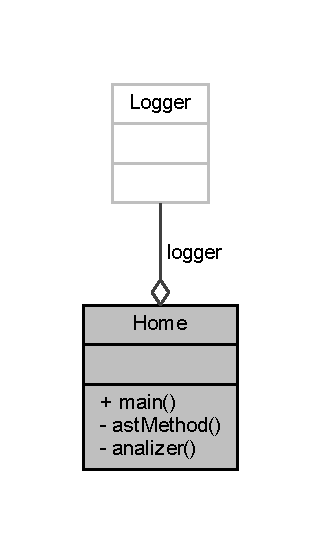
\includegraphics[width=154pt]{class_home__coll__graph}
\end{center}
\end{figure}
\subsection*{Static Public Member Functions}
\begin{DoxyCompactItemize}
\item 
\hypertarget{class_home_a824a2d585cb36f1a452ebc5db9b49ed0}{static void {\bfseries main} (String\mbox{[}$\,$\mbox{]} args)  throws Exception}\label{class_home_a824a2d585cb36f1a452ebc5db9b49ed0}

\end{DoxyCompactItemize}
\subsection*{Static Package Attributes}
\begin{DoxyCompactItemize}
\item 
\hypertarget{class_home_ac74d97ae59ddf53153a62e8790619756}{static Logger {\bfseries logger} = Logger.\-get\-Logger(Home.\-class.\-get\-Name())}\label{class_home_ac74d97ae59ddf53153a62e8790619756}

\end{DoxyCompactItemize}
\subsection*{Static Private Member Functions}
\begin{DoxyCompactItemize}
\item 
\hypertarget{class_home_ac6c6a408dc24c30d02945cd67403d6d1}{static void {\bfseries ast\-Method} (\hyperlink{classinput_parser_1_1_abstract_input_parser}{Abstract\-Input\-Parser} parser)  throws Exception }\label{class_home_ac6c6a408dc24c30d02945cd67403d6d1}

\item 
\hypertarget{class_home_a207d973f0026822784672e07478745aa}{static void {\bfseries analizer} (\hyperlink{classinput_parser_1_1_abstract_input_parser}{Abstract\-Input\-Parser} parser)  throws File\-Not\-Found\-Exception, Exception }\label{class_home_a207d973f0026822784672e07478745aa}

\end{DoxyCompactItemize}


\subsection{Detailed Description}
\begin{DoxyAuthor}{Author}
Paolo Pino 
\end{DoxyAuthor}


Definition at line 27 of file Home.\-java.



The documentation for this class was generated from the following file\-:\begin{DoxyCompactItemize}
\item 
src/Home.\-java\end{DoxyCompactItemize}

\hypertarget{class_home_gui}{\section{Home\-Gui Class Reference}
\label{class_home_gui}\index{Home\-Gui@{Home\-Gui}}
}


The gui access.  




Inheritance diagram for Home\-Gui\-:\nopagebreak
\begin{figure}[H]
\begin{center}
\leavevmode
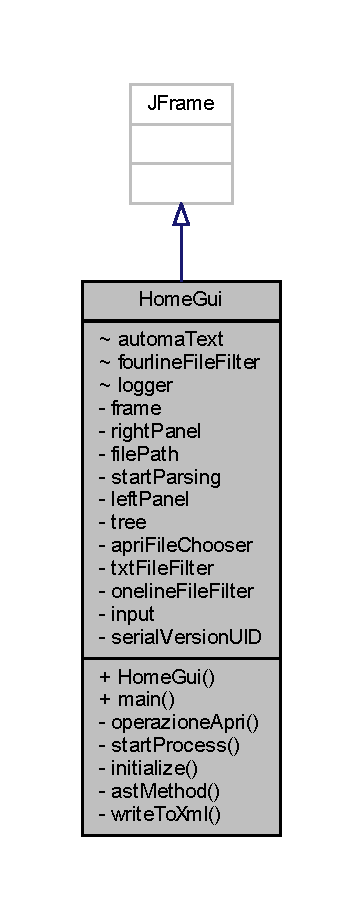
\includegraphics[width=174pt]{class_home_gui__inherit__graph}
\end{center}
\end{figure}


Collaboration diagram for Home\-Gui\-:\nopagebreak
\begin{figure}[H]
\begin{center}
\leavevmode
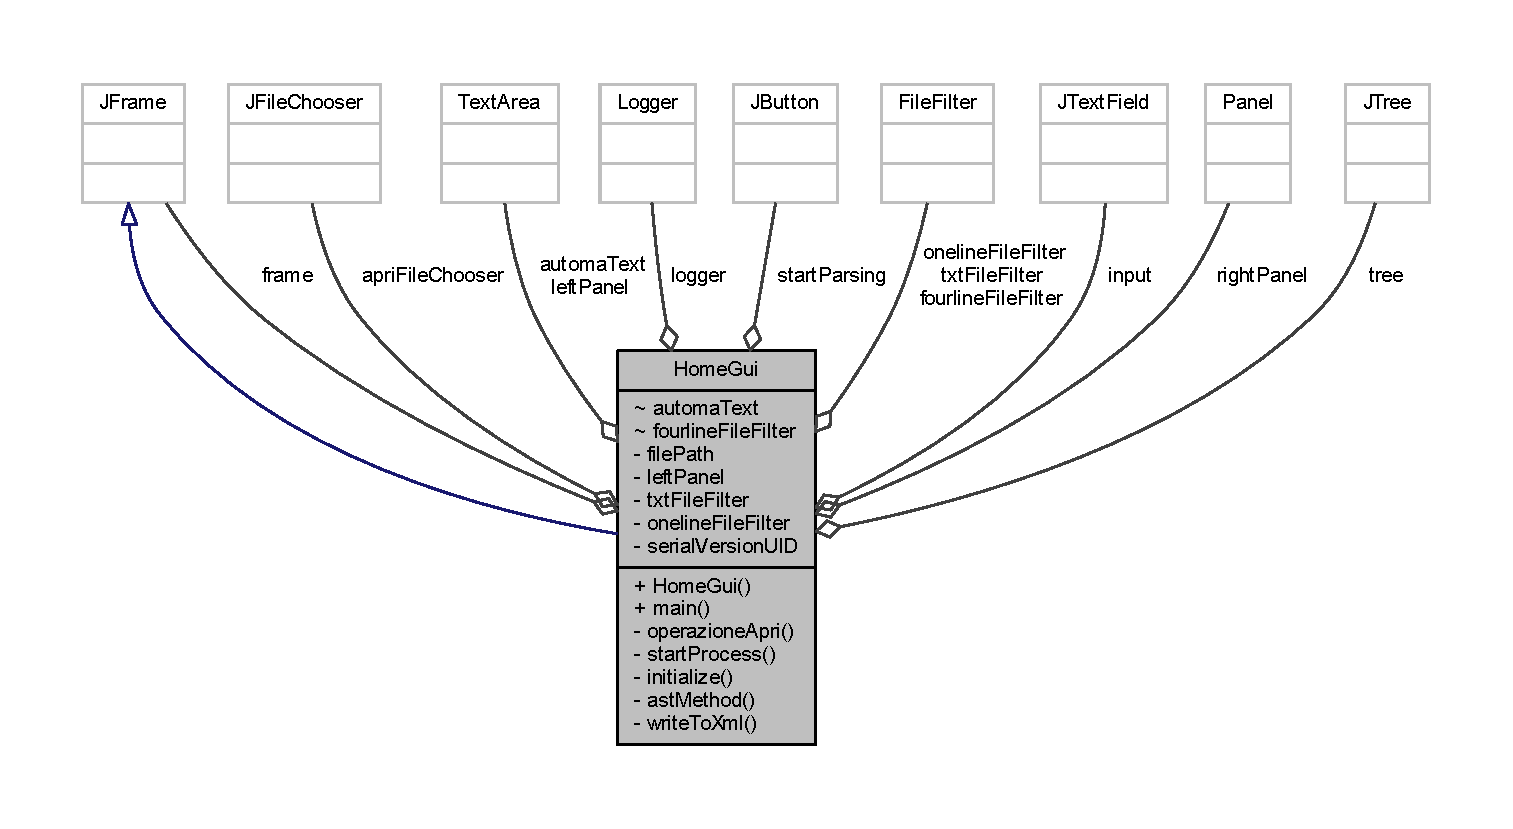
\includegraphics[width=350pt]{class_home_gui__coll__graph}
\end{center}
\end{figure}
\subsection*{Public Member Functions}
\begin{DoxyCompactItemize}
\item 
\hyperlink{class_home_gui_add92e1cf71983b9cc6f70f040d3ea593}{Home\-Gui} ()  throws File\-Not\-Found\-Exception, Exception 
\begin{DoxyCompactList}\small\item\em Initialize G\-U\-I component and start the process. \end{DoxyCompactList}\end{DoxyCompactItemize}
\subsection*{Static Public Member Functions}
\begin{DoxyCompactItemize}
\item 
\hypertarget{class_home_gui_a241867731938068ae82ae7d5e7371fa3}{static void \hyperlink{class_home_gui_a241867731938068ae82ae7d5e7371fa3}{main} (String\mbox{[}$\,$\mbox{]} args)}\label{class_home_gui_a241867731938068ae82ae7d5e7371fa3}

\begin{DoxyCompactList}\small\item\em Launch the application. \end{DoxyCompactList}\end{DoxyCompactItemize}
\subsection*{Package Attributes}
\begin{DoxyCompactItemize}
\item 
\hypertarget{class_home_gui_a6b00edbcb893105ddc5e3b2beb4c2dca}{Text\-Area {\bfseries automa\-Text}}\label{class_home_gui_a6b00edbcb893105ddc5e3b2beb4c2dca}

\item 
\hypertarget{class_home_gui_a7f56e390a2982689b92cee117f50e987}{File\-Filter {\bfseries fourline\-File\-Filter}}\label{class_home_gui_a7f56e390a2982689b92cee117f50e987}

\end{DoxyCompactItemize}
\subsection*{Static Package Attributes}
\begin{DoxyCompactItemize}
\item 
\hypertarget{class_home_gui_a6eef831dc2ff4533740f3395c4b9067a}{static Logger {\bfseries logger} = Logger.\-get\-Logger(Home\-Gui.\-class.\-get\-Name())}\label{class_home_gui_a6eef831dc2ff4533740f3395c4b9067a}

\end{DoxyCompactItemize}
\subsection*{Private Member Functions}
\begin{DoxyCompactItemize}
\item 
\hypertarget{class_home_gui_a8a91bfb188035012962b468a651f73a5}{void {\bfseries operazione\-Apri} ()  throws File\-Not\-Found\-Exception, Exception }\label{class_home_gui_a8a91bfb188035012962b468a651f73a5}

\item 
void \hyperlink{class_home_gui_a52f0602a97cd1ef63063bbbbda036d26}{start\-Process} (String path)  throws File\-Not\-Found\-Exception, Exception 
\begin{DoxyCompactList}\small\item\em Start the parsing of grammar file and create result file. \end{DoxyCompactList}\item 
void \hyperlink{class_home_gui_a5e935834d62fe14dfda2c9884f1f7010}{initialize} ()
\begin{DoxyCompactList}\small\item\em Save operation. \end{DoxyCompactList}\item 
Default\-Mutable\-Tree\-Node \hyperlink{class_home_gui_a2903109ca5fa51fc78f8487c79dafc43}{st\-Method} (\hyperlink{classparser_program_1_1_parser_program}{Parser\-Program} parser\-Program)  throws Exception 
\begin{DoxyCompactList}\small\item\em Create the S\-T. \end{DoxyCompactList}\item 
void \hyperlink{class_home_gui_a0428d3c56abfafc769684835c1581f38}{write\-To\-Xml} (Default\-Mutable\-Tree\-Node root)  throws File\-Not\-Found\-Exception 
\begin{DoxyCompactList}\small\item\em Store an S\-T into xml file named \char`\"{}\-S\-T.\-xml\char`\"{}. \end{DoxyCompactList}\end{DoxyCompactItemize}
\subsection*{Private Attributes}
\begin{DoxyCompactItemize}
\item 
\hypertarget{class_home_gui_a0b1781db25b8fdacc8970aa6166b11ad}{J\-Frame {\bfseries frame}}\label{class_home_gui_a0b1781db25b8fdacc8970aa6166b11ad}

\item 
\hypertarget{class_home_gui_adb0131b6ea64353bf6b0c5993468341c}{Panel {\bfseries right\-Panel}}\label{class_home_gui_adb0131b6ea64353bf6b0c5993468341c}

\item 
\hypertarget{class_home_gui_a1f9226407f1c2c6ff8d62f84dfcebfbe}{String {\bfseries file\-Path}}\label{class_home_gui_a1f9226407f1c2c6ff8d62f84dfcebfbe}

\item 
\hypertarget{class_home_gui_aedb975e31137435a02772599392bf195}{J\-Button {\bfseries start\-Parsing}}\label{class_home_gui_aedb975e31137435a02772599392bf195}

\item 
\hypertarget{class_home_gui_ac6ba89ab2c3204e87ec00b9b4962f327}{Text\-Area {\bfseries left\-Panel}}\label{class_home_gui_ac6ba89ab2c3204e87ec00b9b4962f327}

\item 
\hypertarget{class_home_gui_ab4af4f54e925eedcab3cb87da41410e1}{J\-Tree {\bfseries tree}}\label{class_home_gui_ab4af4f54e925eedcab3cb87da41410e1}

\item 
\hypertarget{class_home_gui_a7b615d195d8208fab52fd9db85082d46}{J\-File\-Chooser {\bfseries apri\-File\-Chooser}}\label{class_home_gui_a7b615d195d8208fab52fd9db85082d46}

\item 
\hypertarget{class_home_gui_af20bf1a94a96e4f53e1f66337a257ce3}{File\-Filter {\bfseries txt\-File\-Filter}}\label{class_home_gui_af20bf1a94a96e4f53e1f66337a257ce3}

\item 
\hypertarget{class_home_gui_a8b0192c597368a34c855abe70a8a80ec}{File\-Filter {\bfseries oneline\-File\-Filter}}\label{class_home_gui_a8b0192c597368a34c855abe70a8a80ec}

\item 
\hypertarget{class_home_gui_ab33ea273ae2f2c5bde32041076af630c}{J\-Text\-Field {\bfseries input}}\label{class_home_gui_ab33ea273ae2f2c5bde32041076af630c}

\end{DoxyCompactItemize}
\subsection*{Static Private Attributes}
\begin{DoxyCompactItemize}
\item 
\hypertarget{class_home_gui_a6a93dac6b8c89a59ca14536d6f5ad414}{static final long {\bfseries serial\-Version\-U\-I\-D} = 1\-L}\label{class_home_gui_a6a93dac6b8c89a59ca14536d6f5ad414}

\end{DoxyCompactItemize}


\subsection{Detailed Description}
The gui access. 

\begin{DoxyAuthor}{Author}
Paolo Pino 
\end{DoxyAuthor}


Definition at line 51 of file Home\-Gui.\-java.



\subsection{Constructor \& Destructor Documentation}
\hypertarget{class_home_gui_add92e1cf71983b9cc6f70f040d3ea593}{\index{Home\-Gui@{Home\-Gui}!Home\-Gui@{Home\-Gui}}
\index{Home\-Gui@{Home\-Gui}!HomeGui@{Home\-Gui}}
\subsubsection[{Home\-Gui}]{\setlength{\rightskip}{0pt plus 5cm}{\bf Home\-Gui.\-Home\-Gui} (
\begin{DoxyParamCaption}
{}
\end{DoxyParamCaption}
)  throws File\-Not\-Found\-Exception, Exception }}\label{class_home_gui_add92e1cf71983b9cc6f70f040d3ea593}


Initialize G\-U\-I component and start the process. 


\begin{DoxyExceptions}{Exceptions}
{\em Exception} & \\
\hline
{\em File\-Not\-Found\-Exception} & \\
\hline
\end{DoxyExceptions}
\begin{DoxyAuthor}{Author}
Paolo Pino 
\end{DoxyAuthor}


Definition at line 86 of file Home\-Gui.\-java.



Here is the call graph for this function\-:\nopagebreak
\begin{figure}[H]
\begin{center}
\leavevmode
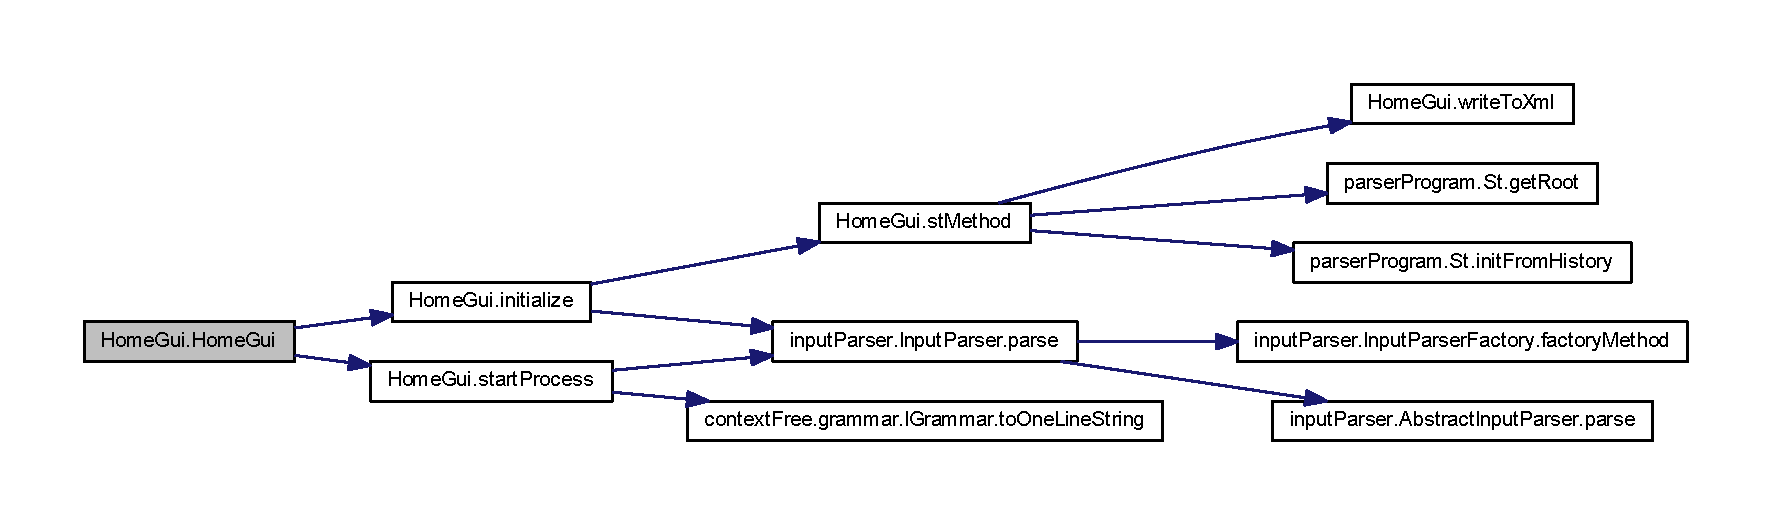
\includegraphics[width=350pt]{class_home_gui_add92e1cf71983b9cc6f70f040d3ea593_cgraph}
\end{center}
\end{figure}




Here is the caller graph for this function\-:\nopagebreak
\begin{figure}[H]
\begin{center}
\leavevmode
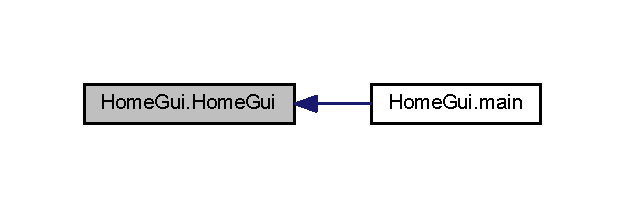
\includegraphics[width=300pt]{class_home_gui_add92e1cf71983b9cc6f70f040d3ea593_icgraph}
\end{center}
\end{figure}




\subsection{Member Function Documentation}
\hypertarget{class_home_gui_a5e935834d62fe14dfda2c9884f1f7010}{\index{Home\-Gui@{Home\-Gui}!initialize@{initialize}}
\index{initialize@{initialize}!HomeGui@{Home\-Gui}}
\subsubsection[{initialize}]{\setlength{\rightskip}{0pt plus 5cm}void {\bf Home\-Gui.\-initialize} (
\begin{DoxyParamCaption}
{}
\end{DoxyParamCaption}
)\hspace{0.3cm}{\ttfamily  \mbox{[}private\mbox{]}}}}\label{class_home_gui_a5e935834d62fe14dfda2c9884f1f7010}


Save operation. 

Initialize the contents of the frame. When clicked parse \char`\"{}\-Result.\-txt\char`\"{} file and create the A\-S\-T. \begin{DoxyAuthor}{Author}
Paolo Pino
\end{DoxyAuthor}


Definition at line 176 of file Home\-Gui.\-java.



Here is the call graph for this function\-:\nopagebreak
\begin{figure}[H]
\begin{center}
\leavevmode
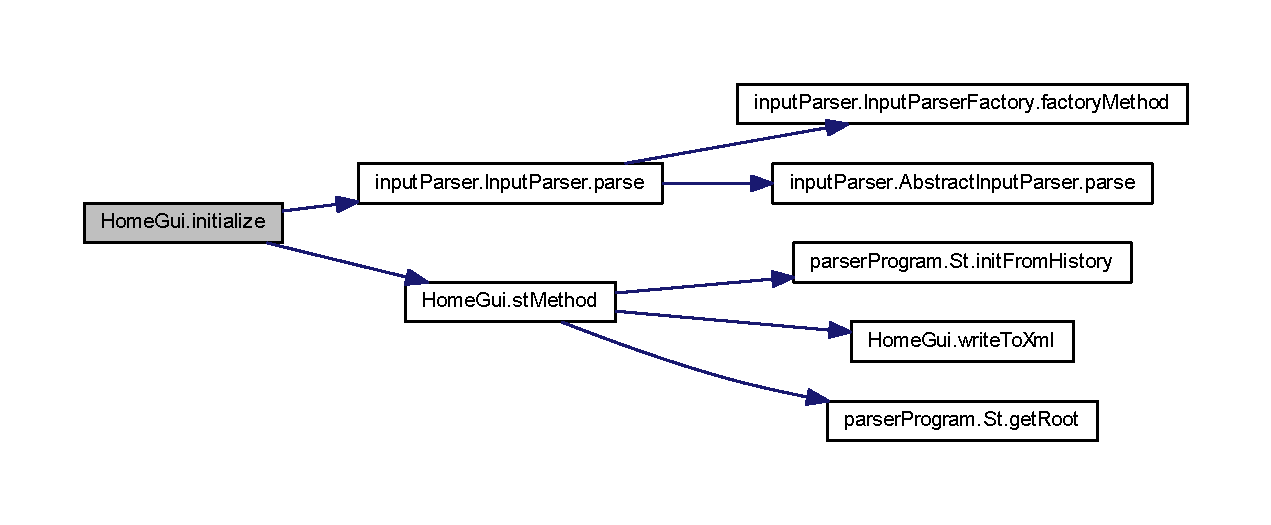
\includegraphics[width=350pt]{class_home_gui_a5e935834d62fe14dfda2c9884f1f7010_cgraph}
\end{center}
\end{figure}




Here is the caller graph for this function\-:\nopagebreak
\begin{figure}[H]
\begin{center}
\leavevmode
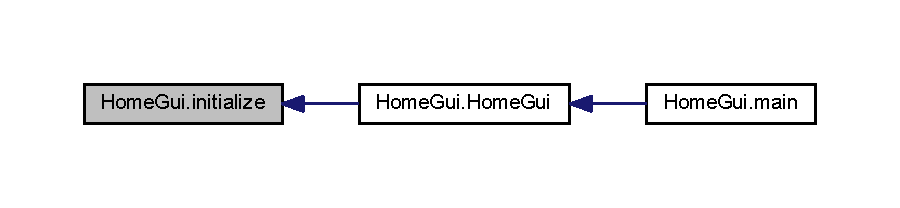
\includegraphics[width=350pt]{class_home_gui_a5e935834d62fe14dfda2c9884f1f7010_icgraph}
\end{center}
\end{figure}


\hypertarget{class_home_gui_a52f0602a97cd1ef63063bbbbda036d26}{\index{Home\-Gui@{Home\-Gui}!start\-Process@{start\-Process}}
\index{start\-Process@{start\-Process}!HomeGui@{Home\-Gui}}
\subsubsection[{start\-Process}]{\setlength{\rightskip}{0pt plus 5cm}void {\bf Home\-Gui.\-start\-Process} (
\begin{DoxyParamCaption}
\item[{String}]{path}
\end{DoxyParamCaption}
)  throws File\-Not\-Found\-Exception, Exception \hspace{0.3cm}{\ttfamily  \mbox{[}private\mbox{]}}}}\label{class_home_gui_a52f0602a97cd1ef63063bbbbda036d26}


Start the parsing of grammar file and create result file. 


\begin{DoxyParams}{Parameters}
{\em path} & the path of grammar file (ex. grammar.\-4l) \\
\hline
\end{DoxyParams}

\begin{DoxyExceptions}{Exceptions}
{\em File\-Not\-Found\-Exception} & \\
\hline
{\em Exception} & \\
\hline
\end{DoxyExceptions}
\begin{DoxyAuthor}{Author}
Paolo Pino 
\end{DoxyAuthor}


Definition at line 127 of file Home\-Gui.\-java.



Here is the call graph for this function\-:\nopagebreak
\begin{figure}[H]
\begin{center}
\leavevmode
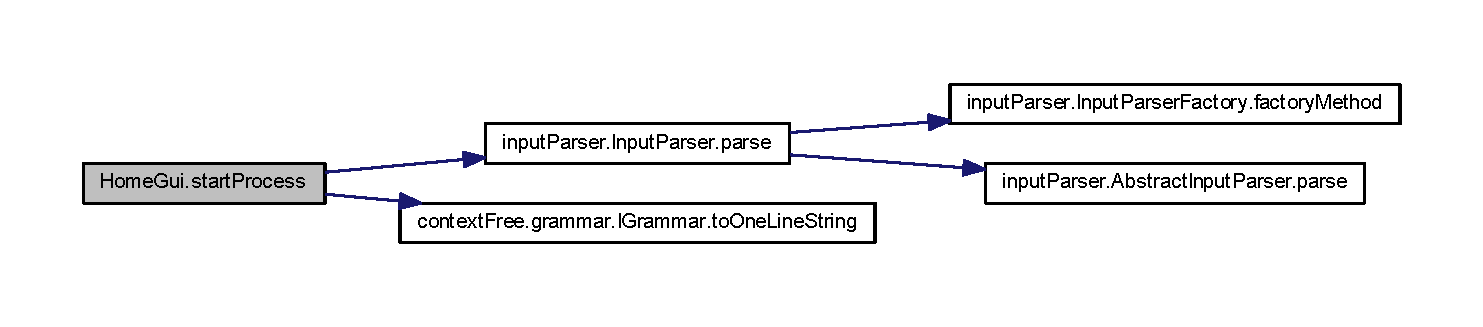
\includegraphics[width=350pt]{class_home_gui_a52f0602a97cd1ef63063bbbbda036d26_cgraph}
\end{center}
\end{figure}




Here is the caller graph for this function\-:\nopagebreak
\begin{figure}[H]
\begin{center}
\leavevmode
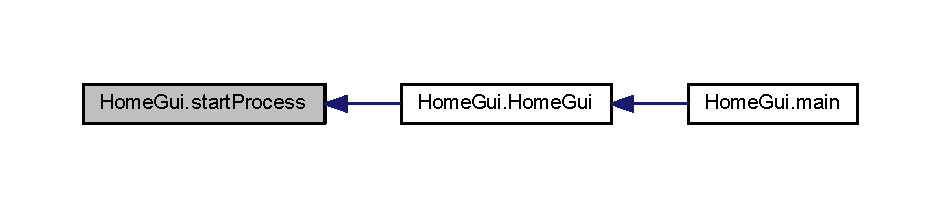
\includegraphics[width=350pt]{class_home_gui_a52f0602a97cd1ef63063bbbbda036d26_icgraph}
\end{center}
\end{figure}


\hypertarget{class_home_gui_a2903109ca5fa51fc78f8487c79dafc43}{\index{Home\-Gui@{Home\-Gui}!st\-Method@{st\-Method}}
\index{st\-Method@{st\-Method}!HomeGui@{Home\-Gui}}
\subsubsection[{st\-Method}]{\setlength{\rightskip}{0pt plus 5cm}Default\-Mutable\-Tree\-Node {\bf Home\-Gui.\-st\-Method} (
\begin{DoxyParamCaption}
\item[{{\bf Parser\-Program}}]{parser\-Program}
\end{DoxyParamCaption}
)  throws Exception \hspace{0.3cm}{\ttfamily  \mbox{[}private\mbox{]}}}}\label{class_home_gui_a2903109ca5fa51fc78f8487c79dafc43}


Create the S\-T. 


\begin{DoxyParams}{Parameters}
{\em parser} & the object that rappresent \char`\"{}\-Result.\-txt\char`\"{} \\
\hline
\end{DoxyParams}
\begin{DoxyReturn}{Returns}
Default\-Mutable\-Tree\-Node root of S\-T 
\end{DoxyReturn}

\begin{DoxyExceptions}{Exceptions}
{\em Exception} & \\
\hline
\end{DoxyExceptions}
\begin{DoxyAuthor}{Author}
Paolo Pino 
\end{DoxyAuthor}


Definition at line 352 of file Home\-Gui.\-java.



Here is the call graph for this function\-:\nopagebreak
\begin{figure}[H]
\begin{center}
\leavevmode
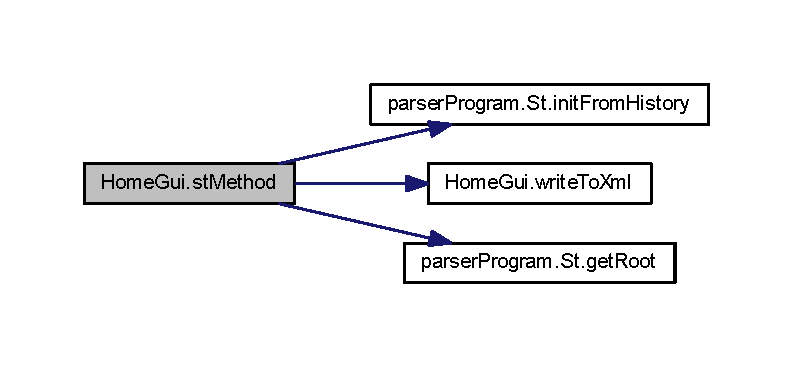
\includegraphics[width=350pt]{class_home_gui_a2903109ca5fa51fc78f8487c79dafc43_cgraph}
\end{center}
\end{figure}




Here is the caller graph for this function\-:\nopagebreak
\begin{figure}[H]
\begin{center}
\leavevmode
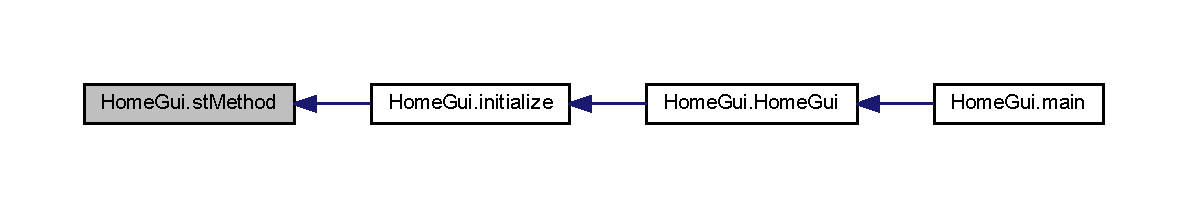
\includegraphics[width=350pt]{class_home_gui_a2903109ca5fa51fc78f8487c79dafc43_icgraph}
\end{center}
\end{figure}


\hypertarget{class_home_gui_a0428d3c56abfafc769684835c1581f38}{\index{Home\-Gui@{Home\-Gui}!write\-To\-Xml@{write\-To\-Xml}}
\index{write\-To\-Xml@{write\-To\-Xml}!HomeGui@{Home\-Gui}}
\subsubsection[{write\-To\-Xml}]{\setlength{\rightskip}{0pt plus 5cm}void {\bf Home\-Gui.\-write\-To\-Xml} (
\begin{DoxyParamCaption}
\item[{Default\-Mutable\-Tree\-Node}]{root}
\end{DoxyParamCaption}
)  throws File\-Not\-Found\-Exception \hspace{0.3cm}{\ttfamily  \mbox{[}private\mbox{]}}}}\label{class_home_gui_a0428d3c56abfafc769684835c1581f38}


Store an S\-T into xml file named \char`\"{}\-S\-T.\-xml\char`\"{}. 


\begin{DoxyParams}{Parameters}
{\em root} & the root of A\-S\-T \\
\hline
\end{DoxyParams}

\begin{DoxyExceptions}{Exceptions}
{\em File\-Not\-Found\-Exception} & \\
\hline
\end{DoxyExceptions}
\begin{DoxyAuthor}{Author}
Paolo Pino 
\end{DoxyAuthor}


Definition at line 380 of file Home\-Gui.\-java.



Here is the caller graph for this function\-:\nopagebreak
\begin{figure}[H]
\begin{center}
\leavevmode
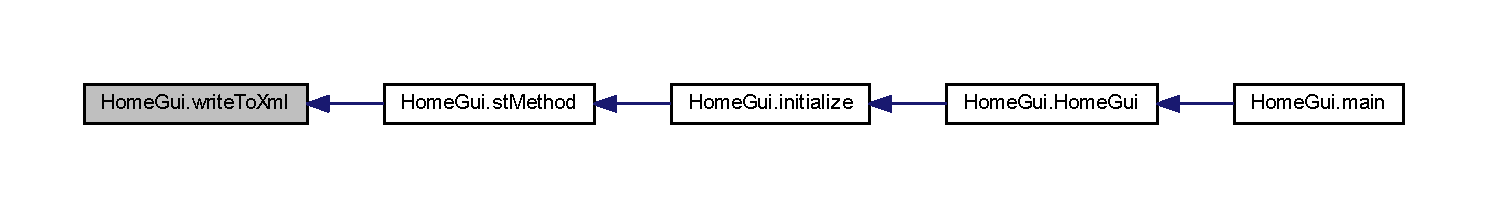
\includegraphics[width=350pt]{class_home_gui_a0428d3c56abfafc769684835c1581f38_icgraph}
\end{center}
\end{figure}




The documentation for this class was generated from the following file\-:\begin{DoxyCompactItemize}
\item 
src/Home\-Gui.\-java\end{DoxyCompactItemize}

\hypertarget{interfacecontext_free_1_1grammar_1_1_i_grammar}{\section{context\-Free.\-grammar.\-I\-Grammar Interface Reference}
\label{interfacecontext_free_1_1grammar_1_1_i_grammar}\index{context\-Free.\-grammar.\-I\-Grammar@{context\-Free.\-grammar.\-I\-Grammar}}
}


Grammar Interface.  




Inheritance diagram for context\-Free.\-grammar.\-I\-Grammar\-:
\nopagebreak
\begin{figure}[H]
\begin{center}
\leavevmode
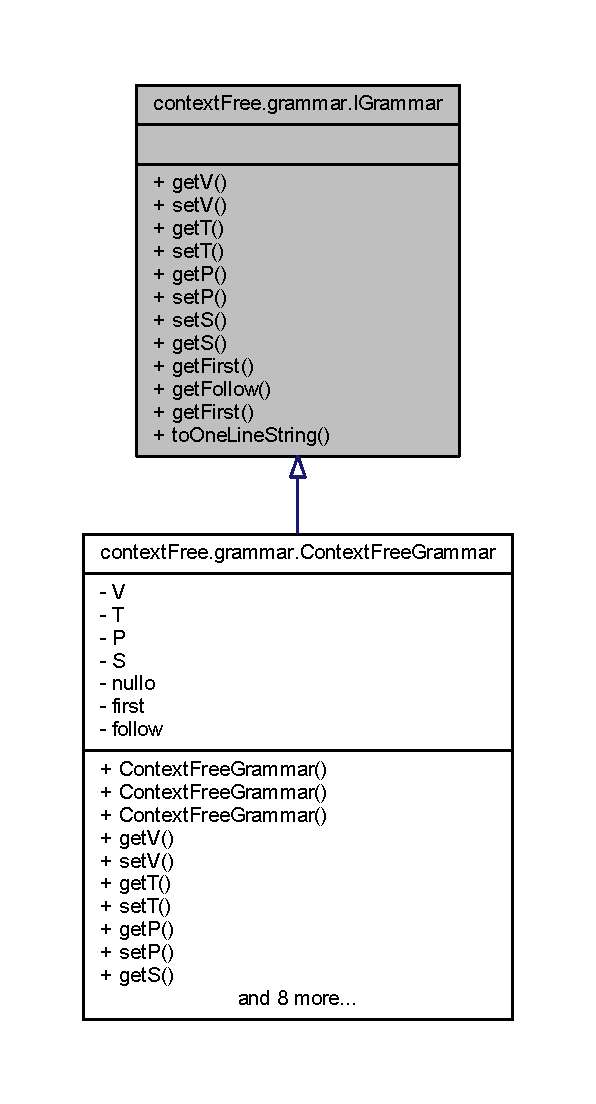
\includegraphics[width=286pt]{interfacecontext_free_1_1grammar_1_1_i_grammar__inherit__graph}
\end{center}
\end{figure}
\subsection*{Public Member Functions}
\begin{DoxyCompactItemize}
\item 
List$<$ String $>$ \hyperlink{interfacecontext_free_1_1grammar_1_1_i_grammar_a4b1bc2134e63051dc37e693294aaeec6}{get\-V} ()
\begin{DoxyCompactList}\small\item\em Get non-\/terminal symbols list. \end{DoxyCompactList}\item 
void \hyperlink{interfacecontext_free_1_1grammar_1_1_i_grammar_ae7bd17123ad7424af06a7da75a6bc745}{set\-V} (List$<$ String $>$ v)
\begin{DoxyCompactList}\small\item\em Set the list of non-\/terminal symbols. \end{DoxyCompactList}\item 
List$<$ String $>$ \hyperlink{interfacecontext_free_1_1grammar_1_1_i_grammar_a996f5e0bed5a6ac469b764f56d420fb1}{get\-T} ()
\begin{DoxyCompactList}\small\item\em Get terminal symbols list. \end{DoxyCompactList}\item 
void \hyperlink{interfacecontext_free_1_1grammar_1_1_i_grammar_a775125de1388036059da1860ae61a100}{set\-T} (List$<$ String $>$ e)
\begin{DoxyCompactList}\small\item\em Set the list of terminal symbols. \end{DoxyCompactList}\item 
List$<$ \hyperlink{classcontext_free_1_1grammar_1_1_production}{Production} $>$ \hyperlink{interfacecontext_free_1_1grammar_1_1_i_grammar_a629ab4dc36a869b93fa239a3fee760f9}{get\-P} ()
\begin{DoxyCompactList}\small\item\em Get production list. \end{DoxyCompactList}\item 
void \hyperlink{interfacecontext_free_1_1grammar_1_1_i_grammar_ac070229e5571e47032b5199c0bf2c354}{set\-P} (List$<$ \hyperlink{classcontext_free_1_1grammar_1_1_production}{Production} $>$ p)
\begin{DoxyCompactList}\small\item\em Set the produciton list. \end{DoxyCompactList}\item 
void \hyperlink{interfacecontext_free_1_1grammar_1_1_i_grammar_a134f8b2183ec804eff78ac57b16a0ab9}{set\-S} (String s)
\begin{DoxyCompactList}\small\item\em Set the axioms for the grammar. \end{DoxyCompactList}\item 
String \hyperlink{interfacecontext_free_1_1grammar_1_1_i_grammar_aceb36e584d26bd39a0f5186742cc9b5b}{get\-S} ()
\begin{DoxyCompactList}\small\item\em Get the axioms. \end{DoxyCompactList}\item 
Set$<$ String $>$\mbox{[}$\,$\mbox{]} \hyperlink{interfacecontext_free_1_1grammar_1_1_i_grammar_a256e9280e008a7c709ccb80725ccc0f2}{get\-First} ()
\begin{DoxyCompactList}\small\item\em Get the list of first for the grammar. \end{DoxyCompactList}\item 
Set$<$ String $>$\mbox{[}$\,$\mbox{]} \hyperlink{interfacecontext_free_1_1grammar_1_1_i_grammar_aad085d9f84a32ca1abe5fba0c9e5f20c}{get\-Follow} ()
\begin{DoxyCompactList}\small\item\em Get the list of follow for the grammar. \end{DoxyCompactList}\item 
Set$<$ String $>$ \hyperlink{interfacecontext_free_1_1grammar_1_1_i_grammar_a7a05f11e88cdbe29db1849541592e272}{get\-First} (String A)
\begin{DoxyCompactList}\small\item\em Get the list of follow for the grammarfor a specific symbol. \end{DoxyCompactList}\item 
String \hyperlink{interfacecontext_free_1_1grammar_1_1_i_grammar_a5fdeb5a6a9426b400c2fe805566a377c}{to\-One\-Line\-String} ()
\end{DoxyCompactItemize}


\subsection{Detailed Description}
Grammar Interface. 

\begin{DoxyAuthor}{Author}
Paolo Pino 
\end{DoxyAuthor}


Definition at line 10 of file I\-Grammar.\-java.



\subsection{Member Function Documentation}
\hypertarget{interfacecontext_free_1_1grammar_1_1_i_grammar_a256e9280e008a7c709ccb80725ccc0f2}{\index{context\-Free\-::grammar\-::\-I\-Grammar@{context\-Free\-::grammar\-::\-I\-Grammar}!get\-First@{get\-First}}
\index{get\-First@{get\-First}!contextFree::grammar::IGrammar@{context\-Free\-::grammar\-::\-I\-Grammar}}
\subsubsection[{get\-First}]{\setlength{\rightskip}{0pt plus 5cm}Set$<$String$>$ \mbox{[}$\,$\mbox{]} {\bf context\-Free.\-grammar.\-I\-Grammar.\-get\-First} (
\begin{DoxyParamCaption}
{}
\end{DoxyParamCaption}
)}}\label{interfacecontext_free_1_1grammar_1_1_i_grammar_a256e9280e008a7c709ccb80725ccc0f2}


Get the list of first for the grammar. 

\begin{DoxyReturn}{Returns}
the first list. 
\end{DoxyReturn}


Implemented in \hyperlink{classcontext_free_1_1grammar_1_1_context_free_grammar_adc3a25917132474960be34329cdaead9}{context\-Free.\-grammar.\-Context\-Free\-Grammar}.



Here is the caller graph for this function\-:
\nopagebreak
\begin{figure}[H]
\begin{center}
\leavevmode
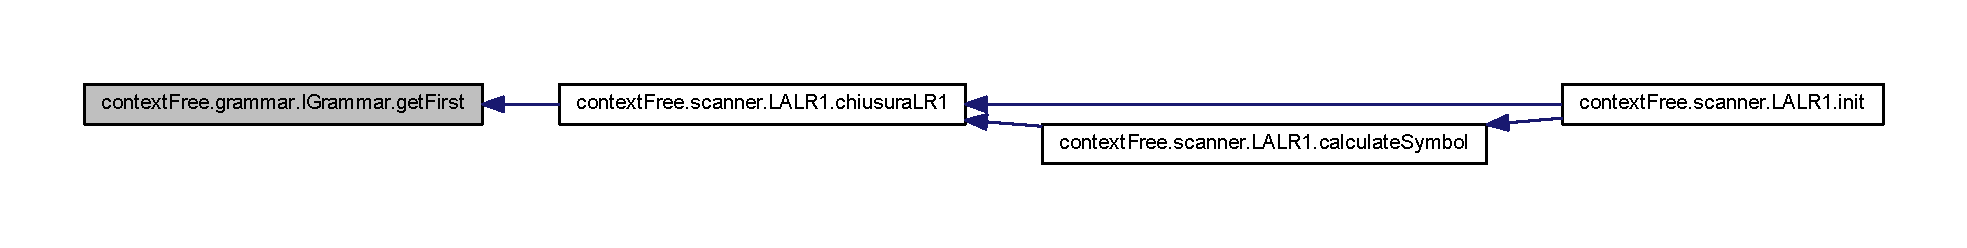
\includegraphics[width=350pt]{interfacecontext_free_1_1grammar_1_1_i_grammar_a256e9280e008a7c709ccb80725ccc0f2_icgraph}
\end{center}
\end{figure}


\hypertarget{interfacecontext_free_1_1grammar_1_1_i_grammar_a7a05f11e88cdbe29db1849541592e272}{\index{context\-Free\-::grammar\-::\-I\-Grammar@{context\-Free\-::grammar\-::\-I\-Grammar}!get\-First@{get\-First}}
\index{get\-First@{get\-First}!contextFree::grammar::IGrammar@{context\-Free\-::grammar\-::\-I\-Grammar}}
\subsubsection[{get\-First}]{\setlength{\rightskip}{0pt plus 5cm}Set$<$String$>$ {\bf context\-Free.\-grammar.\-I\-Grammar.\-get\-First} (
\begin{DoxyParamCaption}
\item[{String}]{A}
\end{DoxyParamCaption}
)}}\label{interfacecontext_free_1_1grammar_1_1_i_grammar_a7a05f11e88cdbe29db1849541592e272}


Get the list of follow for the grammarfor a specific symbol. 

\begin{DoxyReturn}{Returns}
the follow list. 
\end{DoxyReturn}


Implemented in \hyperlink{classcontext_free_1_1grammar_1_1_context_free_grammar_a2140cdc636585e9714e8dc42c936eee5}{context\-Free.\-grammar.\-Context\-Free\-Grammar}.

\hypertarget{interfacecontext_free_1_1grammar_1_1_i_grammar_aad085d9f84a32ca1abe5fba0c9e5f20c}{\index{context\-Free\-::grammar\-::\-I\-Grammar@{context\-Free\-::grammar\-::\-I\-Grammar}!get\-Follow@{get\-Follow}}
\index{get\-Follow@{get\-Follow}!contextFree::grammar::IGrammar@{context\-Free\-::grammar\-::\-I\-Grammar}}
\subsubsection[{get\-Follow}]{\setlength{\rightskip}{0pt plus 5cm}Set$<$String$>$ \mbox{[}$\,$\mbox{]} {\bf context\-Free.\-grammar.\-I\-Grammar.\-get\-Follow} (
\begin{DoxyParamCaption}
{}
\end{DoxyParamCaption}
)}}\label{interfacecontext_free_1_1grammar_1_1_i_grammar_aad085d9f84a32ca1abe5fba0c9e5f20c}


Get the list of follow for the grammar. 

\begin{DoxyReturn}{Returns}
the follow list. 
\end{DoxyReturn}


Implemented in \hyperlink{classcontext_free_1_1grammar_1_1_context_free_grammar_a5dae0e5de95349d310869fb5941cb5be}{context\-Free.\-grammar.\-Context\-Free\-Grammar}.

\hypertarget{interfacecontext_free_1_1grammar_1_1_i_grammar_a629ab4dc36a869b93fa239a3fee760f9}{\index{context\-Free\-::grammar\-::\-I\-Grammar@{context\-Free\-::grammar\-::\-I\-Grammar}!get\-P@{get\-P}}
\index{get\-P@{get\-P}!contextFree::grammar::IGrammar@{context\-Free\-::grammar\-::\-I\-Grammar}}
\subsubsection[{get\-P}]{\setlength{\rightskip}{0pt plus 5cm}List$<${\bf Production}$>$ {\bf context\-Free.\-grammar.\-I\-Grammar.\-get\-P} (
\begin{DoxyParamCaption}
{}
\end{DoxyParamCaption}
)}}\label{interfacecontext_free_1_1grammar_1_1_i_grammar_a629ab4dc36a869b93fa239a3fee760f9}


Get production list. 

\begin{DoxyReturn}{Returns}
a list of production objects. 
\end{DoxyReturn}


Implemented in \hyperlink{classcontext_free_1_1grammar_1_1_context_free_grammar_ad00a00b018844cf2acb0c1c5f5d97468}{context\-Free.\-grammar.\-Context\-Free\-Grammar}.



Here is the caller graph for this function\-:
\nopagebreak
\begin{figure}[H]
\begin{center}
\leavevmode
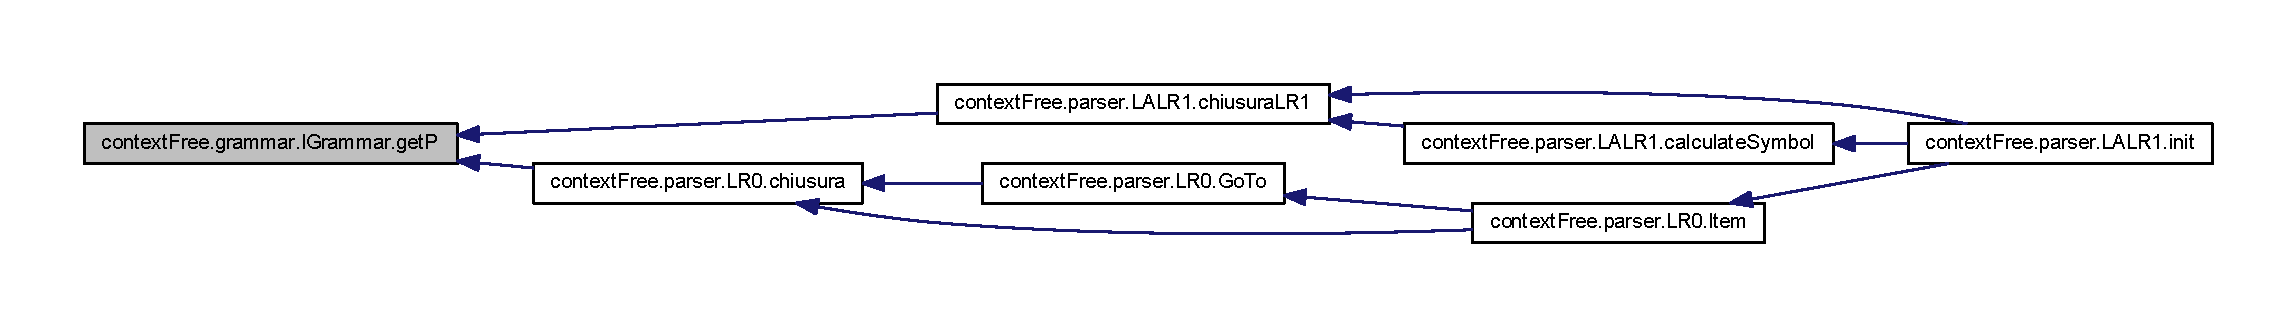
\includegraphics[width=350pt]{interfacecontext_free_1_1grammar_1_1_i_grammar_a629ab4dc36a869b93fa239a3fee760f9_icgraph}
\end{center}
\end{figure}


\hypertarget{interfacecontext_free_1_1grammar_1_1_i_grammar_aceb36e584d26bd39a0f5186742cc9b5b}{\index{context\-Free\-::grammar\-::\-I\-Grammar@{context\-Free\-::grammar\-::\-I\-Grammar}!get\-S@{get\-S}}
\index{get\-S@{get\-S}!contextFree::grammar::IGrammar@{context\-Free\-::grammar\-::\-I\-Grammar}}
\subsubsection[{get\-S}]{\setlength{\rightskip}{0pt plus 5cm}String {\bf context\-Free.\-grammar.\-I\-Grammar.\-get\-S} (
\begin{DoxyParamCaption}
{}
\end{DoxyParamCaption}
)}}\label{interfacecontext_free_1_1grammar_1_1_i_grammar_aceb36e584d26bd39a0f5186742cc9b5b}


Get the axioms. 

\begin{DoxyReturn}{Returns}
the axioms 
\end{DoxyReturn}


Implemented in \hyperlink{classcontext_free_1_1grammar_1_1_context_free_grammar_ad278c4f5e2bdec1d011d11a3008d8754}{context\-Free.\-grammar.\-Context\-Free\-Grammar}.



Here is the caller graph for this function\-:
\nopagebreak
\begin{figure}[H]
\begin{center}
\leavevmode
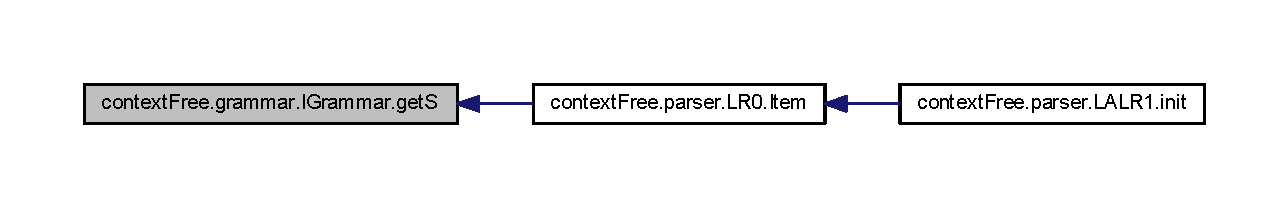
\includegraphics[width=350pt]{interfacecontext_free_1_1grammar_1_1_i_grammar_aceb36e584d26bd39a0f5186742cc9b5b_icgraph}
\end{center}
\end{figure}


\hypertarget{interfacecontext_free_1_1grammar_1_1_i_grammar_a996f5e0bed5a6ac469b764f56d420fb1}{\index{context\-Free\-::grammar\-::\-I\-Grammar@{context\-Free\-::grammar\-::\-I\-Grammar}!get\-T@{get\-T}}
\index{get\-T@{get\-T}!contextFree::grammar::IGrammar@{context\-Free\-::grammar\-::\-I\-Grammar}}
\subsubsection[{get\-T}]{\setlength{\rightskip}{0pt plus 5cm}List$<$String$>$ {\bf context\-Free.\-grammar.\-I\-Grammar.\-get\-T} (
\begin{DoxyParamCaption}
{}
\end{DoxyParamCaption}
)}}\label{interfacecontext_free_1_1grammar_1_1_i_grammar_a996f5e0bed5a6ac469b764f56d420fb1}


Get terminal symbols list. 

\begin{DoxyReturn}{Returns}
a list of string with terminal symbol 
\end{DoxyReturn}


Implemented in \hyperlink{classcontext_free_1_1grammar_1_1_context_free_grammar_a75f1bbf1e0d1d1350032c628779fcffd}{context\-Free.\-grammar.\-Context\-Free\-Grammar}.



Here is the caller graph for this function\-:
\nopagebreak
\begin{figure}[H]
\begin{center}
\leavevmode
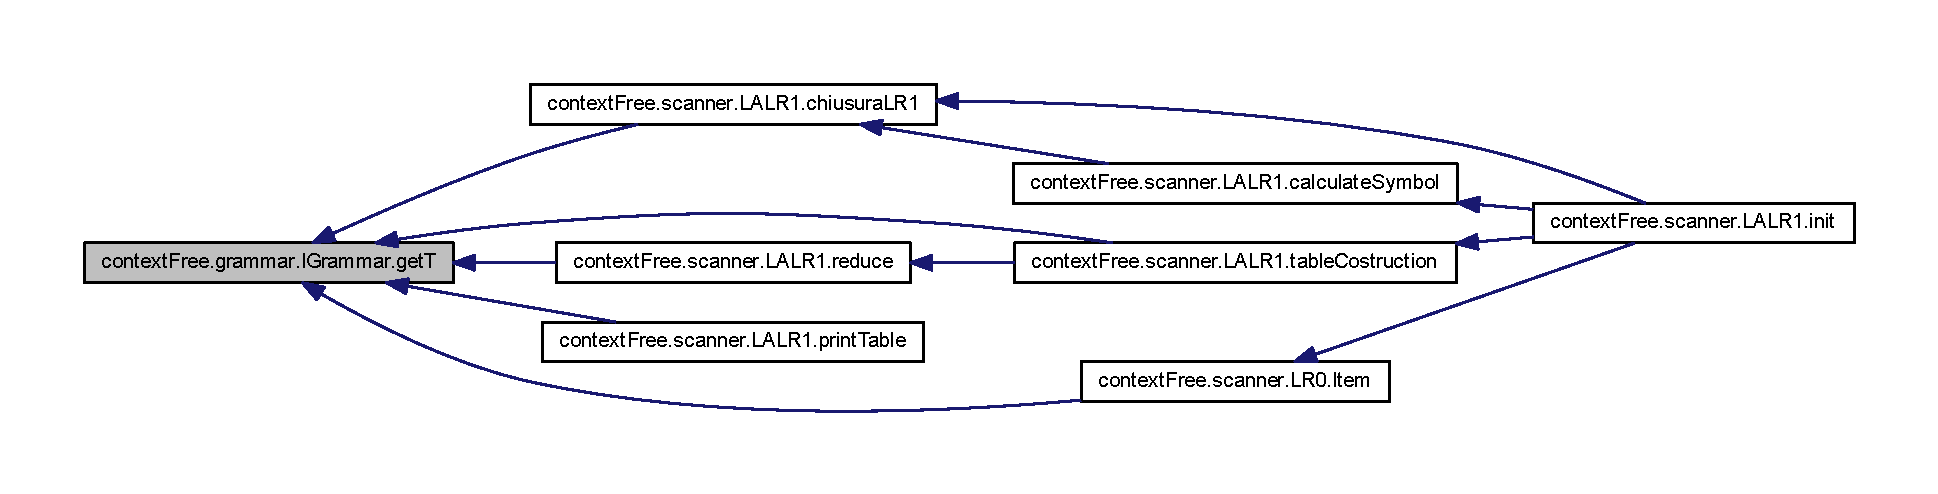
\includegraphics[width=350pt]{interfacecontext_free_1_1grammar_1_1_i_grammar_a996f5e0bed5a6ac469b764f56d420fb1_icgraph}
\end{center}
\end{figure}


\hypertarget{interfacecontext_free_1_1grammar_1_1_i_grammar_a4b1bc2134e63051dc37e693294aaeec6}{\index{context\-Free\-::grammar\-::\-I\-Grammar@{context\-Free\-::grammar\-::\-I\-Grammar}!get\-V@{get\-V}}
\index{get\-V@{get\-V}!contextFree::grammar::IGrammar@{context\-Free\-::grammar\-::\-I\-Grammar}}
\subsubsection[{get\-V}]{\setlength{\rightskip}{0pt plus 5cm}List$<$String$>$ {\bf context\-Free.\-grammar.\-I\-Grammar.\-get\-V} (
\begin{DoxyParamCaption}
{}
\end{DoxyParamCaption}
)}}\label{interfacecontext_free_1_1grammar_1_1_i_grammar_a4b1bc2134e63051dc37e693294aaeec6}


Get non-\/terminal symbols list. 

\begin{DoxyReturn}{Returns}
a list of string with non-\/terminal symbol 
\end{DoxyReturn}


Implemented in \hyperlink{classcontext_free_1_1grammar_1_1_context_free_grammar_a664b69a446100c7c4e7a390fb2ee5ebc}{context\-Free.\-grammar.\-Context\-Free\-Grammar}.



Here is the caller graph for this function\-:
\nopagebreak
\begin{figure}[H]
\begin{center}
\leavevmode
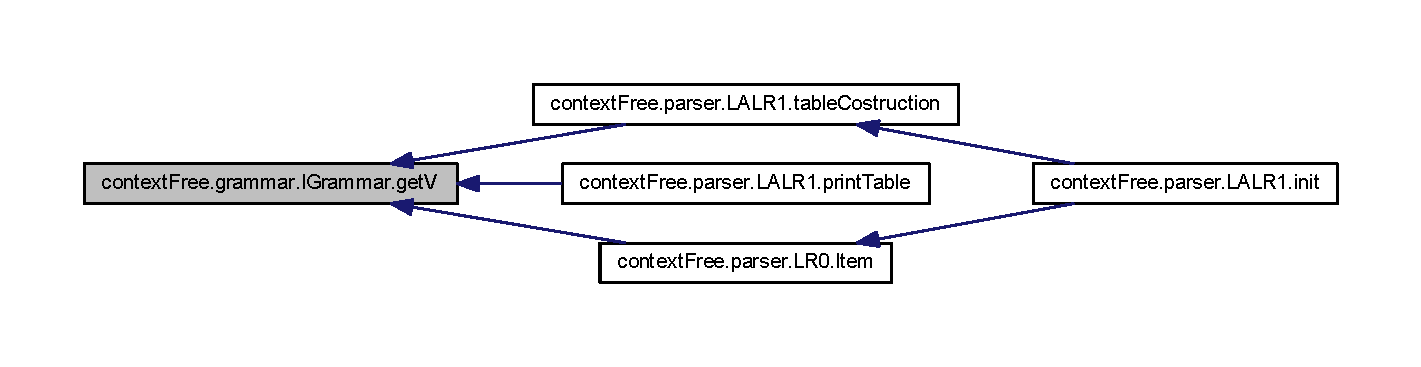
\includegraphics[width=350pt]{interfacecontext_free_1_1grammar_1_1_i_grammar_a4b1bc2134e63051dc37e693294aaeec6_icgraph}
\end{center}
\end{figure}


\hypertarget{interfacecontext_free_1_1grammar_1_1_i_grammar_ac070229e5571e47032b5199c0bf2c354}{\index{context\-Free\-::grammar\-::\-I\-Grammar@{context\-Free\-::grammar\-::\-I\-Grammar}!set\-P@{set\-P}}
\index{set\-P@{set\-P}!contextFree::grammar::IGrammar@{context\-Free\-::grammar\-::\-I\-Grammar}}
\subsubsection[{set\-P}]{\setlength{\rightskip}{0pt plus 5cm}void {\bf context\-Free.\-grammar.\-I\-Grammar.\-set\-P} (
\begin{DoxyParamCaption}
\item[{List$<$ {\bf Production} $>$}]{p}
\end{DoxyParamCaption}
)}}\label{interfacecontext_free_1_1grammar_1_1_i_grammar_ac070229e5571e47032b5199c0bf2c354}


Set the produciton list. 


\begin{DoxyParams}{Parameters}
{\em p} & the list of productions that must be setted. \\
\hline
\end{DoxyParams}


Implemented in \hyperlink{classcontext_free_1_1grammar_1_1_context_free_grammar_a2a66695521702040224c23898b579c92}{context\-Free.\-grammar.\-Context\-Free\-Grammar}.

\hypertarget{interfacecontext_free_1_1grammar_1_1_i_grammar_a134f8b2183ec804eff78ac57b16a0ab9}{\index{context\-Free\-::grammar\-::\-I\-Grammar@{context\-Free\-::grammar\-::\-I\-Grammar}!set\-S@{set\-S}}
\index{set\-S@{set\-S}!contextFree::grammar::IGrammar@{context\-Free\-::grammar\-::\-I\-Grammar}}
\subsubsection[{set\-S}]{\setlength{\rightskip}{0pt plus 5cm}void {\bf context\-Free.\-grammar.\-I\-Grammar.\-set\-S} (
\begin{DoxyParamCaption}
\item[{String}]{s}
\end{DoxyParamCaption}
)}}\label{interfacecontext_free_1_1grammar_1_1_i_grammar_a134f8b2183ec804eff78ac57b16a0ab9}


Set the axioms for the grammar. 


\begin{DoxyParams}{Parameters}
{\em s} & the axioms. \\
\hline
\end{DoxyParams}


Implemented in \hyperlink{classcontext_free_1_1grammar_1_1_context_free_grammar_a2f4c3ec7270d799ed127cb162e0213b3}{context\-Free.\-grammar.\-Context\-Free\-Grammar}.

\hypertarget{interfacecontext_free_1_1grammar_1_1_i_grammar_a775125de1388036059da1860ae61a100}{\index{context\-Free\-::grammar\-::\-I\-Grammar@{context\-Free\-::grammar\-::\-I\-Grammar}!set\-T@{set\-T}}
\index{set\-T@{set\-T}!contextFree::grammar::IGrammar@{context\-Free\-::grammar\-::\-I\-Grammar}}
\subsubsection[{set\-T}]{\setlength{\rightskip}{0pt plus 5cm}void {\bf context\-Free.\-grammar.\-I\-Grammar.\-set\-T} (
\begin{DoxyParamCaption}
\item[{List$<$ String $>$}]{e}
\end{DoxyParamCaption}
)}}\label{interfacecontext_free_1_1grammar_1_1_i_grammar_a775125de1388036059da1860ae61a100}


Set the list of terminal symbols. 


\begin{DoxyParams}{Parameters}
{\em e} & the list of terminal \\
\hline
\end{DoxyParams}


Implemented in \hyperlink{classcontext_free_1_1grammar_1_1_context_free_grammar_aa1c9a277d660b2ba8443f47cb9543811}{context\-Free.\-grammar.\-Context\-Free\-Grammar}.

\hypertarget{interfacecontext_free_1_1grammar_1_1_i_grammar_ae7bd17123ad7424af06a7da75a6bc745}{\index{context\-Free\-::grammar\-::\-I\-Grammar@{context\-Free\-::grammar\-::\-I\-Grammar}!set\-V@{set\-V}}
\index{set\-V@{set\-V}!contextFree::grammar::IGrammar@{context\-Free\-::grammar\-::\-I\-Grammar}}
\subsubsection[{set\-V}]{\setlength{\rightskip}{0pt plus 5cm}void {\bf context\-Free.\-grammar.\-I\-Grammar.\-set\-V} (
\begin{DoxyParamCaption}
\item[{List$<$ String $>$}]{v}
\end{DoxyParamCaption}
)}}\label{interfacecontext_free_1_1grammar_1_1_i_grammar_ae7bd17123ad7424af06a7da75a6bc745}


Set the list of non-\/terminal symbols. 


\begin{DoxyParams}{Parameters}
{\em v} & the list of non-\/terminal \\
\hline
\end{DoxyParams}


Implemented in \hyperlink{classcontext_free_1_1grammar_1_1_context_free_grammar_ad3d3e1efadeb4cc6ed252342fd52c76c}{context\-Free.\-grammar.\-Context\-Free\-Grammar}.

\hypertarget{interfacecontext_free_1_1grammar_1_1_i_grammar_a5fdeb5a6a9426b400c2fe805566a377c}{\index{context\-Free\-::grammar\-::\-I\-Grammar@{context\-Free\-::grammar\-::\-I\-Grammar}!to\-One\-Line\-String@{to\-One\-Line\-String}}
\index{to\-One\-Line\-String@{to\-One\-Line\-String}!contextFree::grammar::IGrammar@{context\-Free\-::grammar\-::\-I\-Grammar}}
\subsubsection[{to\-One\-Line\-String}]{\setlength{\rightskip}{0pt plus 5cm}String {\bf context\-Free.\-grammar.\-I\-Grammar.\-to\-One\-Line\-String} (
\begin{DoxyParamCaption}
{}
\end{DoxyParamCaption}
)}}\label{interfacecontext_free_1_1grammar_1_1_i_grammar_a5fdeb5a6a9426b400c2fe805566a377c}
\begin{DoxyReturn}{Returns}
the grammar string formatted in one line. 
\end{DoxyReturn}


Implemented in \hyperlink{classcontext_free_1_1grammar_1_1_context_free_grammar_a922203e2db862d2a8ab31e8e7736273b}{context\-Free.\-grammar.\-Context\-Free\-Grammar}.



Here is the caller graph for this function\-:
\nopagebreak
\begin{figure}[H]
\begin{center}
\leavevmode
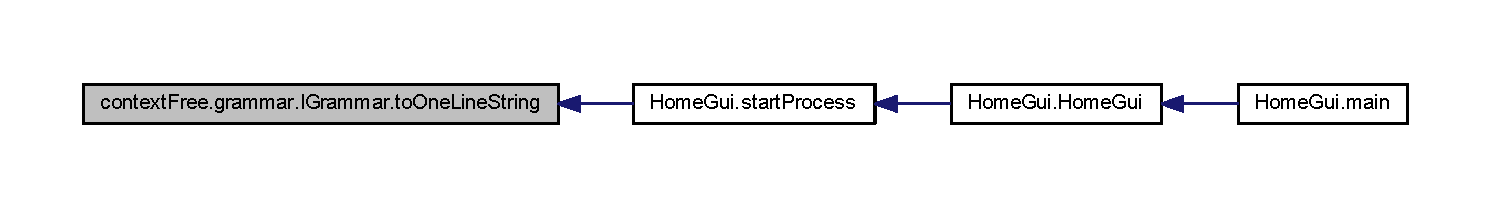
\includegraphics[width=350pt]{interfacecontext_free_1_1grammar_1_1_i_grammar_a5fdeb5a6a9426b400c2fe805566a377c_icgraph}
\end{center}
\end{figure}




The documentation for this interface was generated from the following file\-:\begin{DoxyCompactItemize}
\item 
src/context\-Free/grammar/I\-Grammar.\-java\end{DoxyCompactItemize}

\hypertarget{classcontext_free_1_1parser_1_1_indexed_production}{\section{context\-Free.\-parser.\-Indexed\-Production Class Reference}
\label{classcontext_free_1_1parser_1_1_indexed_production}\index{context\-Free.\-parser.\-Indexed\-Production@{context\-Free.\-parser.\-Indexed\-Production}}
}


Inheritance diagram for context\-Free.\-parser.\-Indexed\-Production\-:
\nopagebreak
\begin{figure}[H]
\begin{center}
\leavevmode
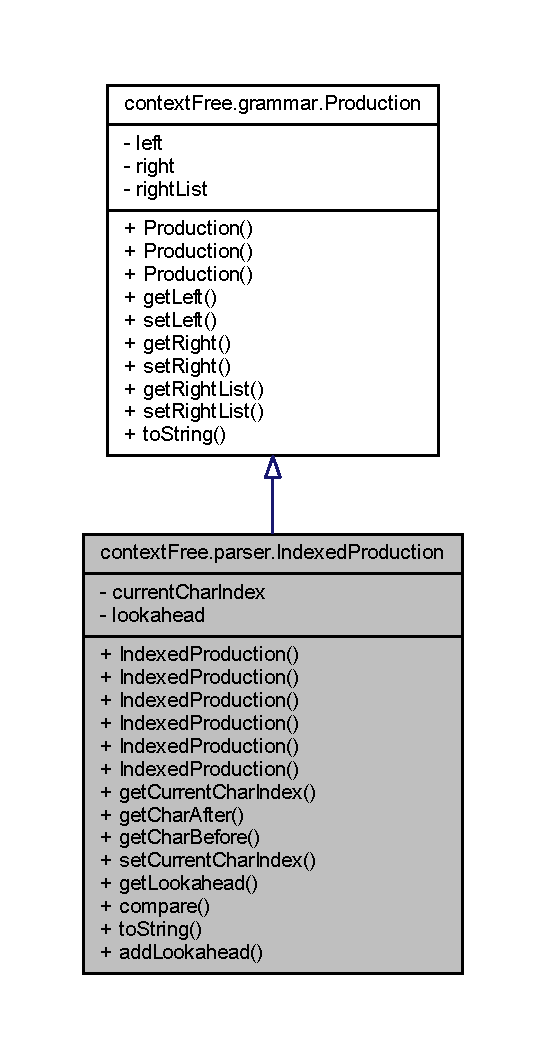
\includegraphics[width=262pt]{classcontext_free_1_1parser_1_1_indexed_production__inherit__graph}
\end{center}
\end{figure}


Collaboration diagram for context\-Free.\-parser.\-Indexed\-Production\-:
\nopagebreak
\begin{figure}[H]
\begin{center}
\leavevmode
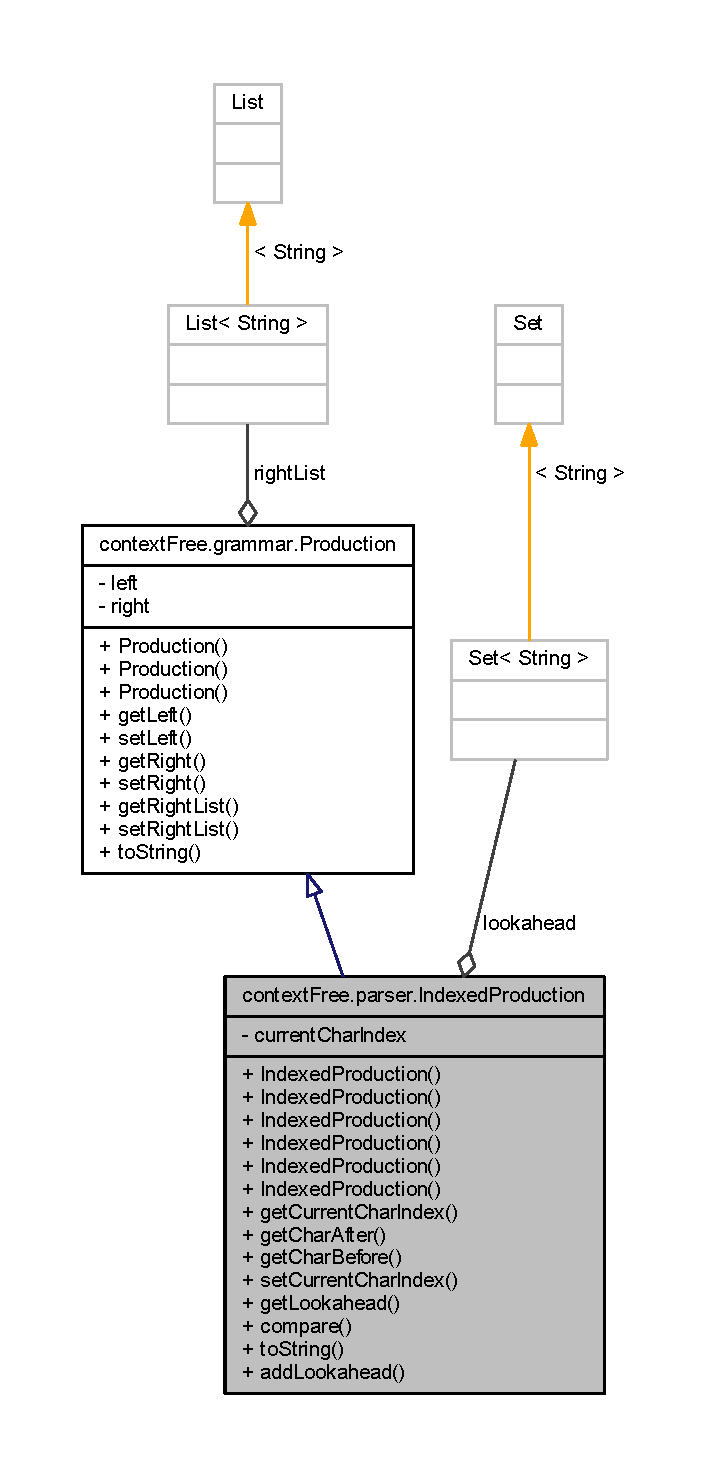
\includegraphics[height=550pt]{classcontext_free_1_1parser_1_1_indexed_production__coll__graph}
\end{center}
\end{figure}
\subsection*{Public Member Functions}
\begin{DoxyCompactItemize}
\item 
\hypertarget{classcontext_free_1_1parser_1_1_indexed_production_a7c67c63baac69c30e9887c0234fd35d9}{{\bfseries Indexed\-Production} (\hyperlink{classcontext_free_1_1parser_1_1_indexed_production}{Indexed\-Production} pro)}\label{classcontext_free_1_1parser_1_1_indexed_production_a7c67c63baac69c30e9887c0234fd35d9}

\item 
\hypertarget{classcontext_free_1_1parser_1_1_indexed_production_a33ac7cade5d7f2a750e07f3b7f7983ac}{{\bfseries Indexed\-Production} (\hyperlink{classcontext_free_1_1grammar_1_1_production}{Production} p)}\label{classcontext_free_1_1parser_1_1_indexed_production_a33ac7cade5d7f2a750e07f3b7f7983ac}

\item 
\hypertarget{classcontext_free_1_1parser_1_1_indexed_production_ac1615174ca96db64a5adfdabd768f9d5}{{\bfseries Indexed\-Production} (int i, \hyperlink{classcontext_free_1_1grammar_1_1_production}{Production} p)}\label{classcontext_free_1_1parser_1_1_indexed_production_ac1615174ca96db64a5adfdabd768f9d5}

\item 
\hypertarget{classcontext_free_1_1parser_1_1_indexed_production_aa1754311192ad2f5c0332025dd162e5f}{{\bfseries Indexed\-Production} (int i, \hyperlink{classcontext_free_1_1grammar_1_1_production}{Production} p, String la)}\label{classcontext_free_1_1parser_1_1_indexed_production_aa1754311192ad2f5c0332025dd162e5f}

\item 
\hypertarget{classcontext_free_1_1parser_1_1_indexed_production_af2e1718023e522ef94aac862ab72307b}{{\bfseries Indexed\-Production} (\hyperlink{classcontext_free_1_1grammar_1_1_production}{Production} p, Set$<$ String $>$ la)}\label{classcontext_free_1_1parser_1_1_indexed_production_af2e1718023e522ef94aac862ab72307b}

\item 
\hypertarget{classcontext_free_1_1parser_1_1_indexed_production_aef48dbe23561cee5a0b744978d1ac2c7}{int {\bfseries get\-Current\-Char\-Index} ()}\label{classcontext_free_1_1parser_1_1_indexed_production_aef48dbe23561cee5a0b744978d1ac2c7}

\item 
String \hyperlink{classcontext_free_1_1parser_1_1_indexed_production_a498db47a05e7f10e580d689e925193b4}{get\-Char\-After} ()
\begin{DoxyCompactList}\small\item\em Return the next character that that will be read. \end{DoxyCompactList}\item 
\hypertarget{classcontext_free_1_1parser_1_1_indexed_production_a143a99e7bf0e81789ee79f514aa3d575}{String {\bfseries get\-Char\-Before} ()}\label{classcontext_free_1_1parser_1_1_indexed_production_a143a99e7bf0e81789ee79f514aa3d575}

\item 
\hypertarget{classcontext_free_1_1parser_1_1_indexed_production_a9673f863b315e7cff584048585906718}{void {\bfseries set\-Current\-Char\-Index} (int current\-Char\-Index)}\label{classcontext_free_1_1parser_1_1_indexed_production_a9673f863b315e7cff584048585906718}

\item 
Set$<$ String $>$ \hyperlink{classcontext_free_1_1parser_1_1_indexed_production_a94e0e318a96518ee50607e682e7f0382}{get\-Lookahead} ()
\item 
boolean \hyperlink{classcontext_free_1_1parser_1_1_indexed_production_aa79a2e2cbbc1f35d6416647d80daf3d8}{compare} (\hyperlink{classcontext_free_1_1parser_1_1_indexed_production}{Indexed\-Production} p)
\begin{DoxyCompactList}\small\item\em Compare to production without the dot. \end{DoxyCompactList}\item 
\hypertarget{classcontext_free_1_1parser_1_1_indexed_production_a061cd84bd37e6111edcd52bcb5b9c749}{String \hyperlink{classcontext_free_1_1parser_1_1_indexed_production_a061cd84bd37e6111edcd52bcb5b9c749}{to\-String} ()}\label{classcontext_free_1_1parser_1_1_indexed_production_a061cd84bd37e6111edcd52bcb5b9c749}

\begin{DoxyCompactList}\small\item\em return a formatted string in the form axioms \-:\-: = expression \end{DoxyCompactList}\item 
\hypertarget{classcontext_free_1_1parser_1_1_indexed_production_ae6af99251737ae274afc4028fa6eb13e}{boolean {\bfseries add\-Lookahead} (Set$<$ String $>$ lookahead2)}\label{classcontext_free_1_1parser_1_1_indexed_production_ae6af99251737ae274afc4028fa6eb13e}

\end{DoxyCompactItemize}
\subsection*{Private Attributes}
\begin{DoxyCompactItemize}
\item 
\hypertarget{classcontext_free_1_1parser_1_1_indexed_production_a8ed426b66a378ce272cc13ae397e52cd}{int {\bfseries current\-Char\-Index}}\label{classcontext_free_1_1parser_1_1_indexed_production_a8ed426b66a378ce272cc13ae397e52cd}

\item 
\hypertarget{classcontext_free_1_1parser_1_1_indexed_production_a58e8935cd1c81a767b47b4d31c87b35c}{Set$<$ String $>$ {\bfseries lookahead}}\label{classcontext_free_1_1parser_1_1_indexed_production_a58e8935cd1c81a767b47b4d31c87b35c}

\end{DoxyCompactItemize}


\subsection{Detailed Description}


Definition at line 10 of file Indexed\-Production.\-java.



\subsection{Member Function Documentation}
\hypertarget{classcontext_free_1_1parser_1_1_indexed_production_aa79a2e2cbbc1f35d6416647d80daf3d8}{\index{context\-Free\-::parser\-::\-Indexed\-Production@{context\-Free\-::parser\-::\-Indexed\-Production}!compare@{compare}}
\index{compare@{compare}!contextFree::parser::IndexedProduction@{context\-Free\-::parser\-::\-Indexed\-Production}}
\subsubsection[{compare}]{\setlength{\rightskip}{0pt plus 5cm}boolean {\bf context\-Free.\-parser.\-Indexed\-Production.\-compare} (
\begin{DoxyParamCaption}
\item[{{\bf Indexed\-Production}}]{p}
\end{DoxyParamCaption}
)}}\label{classcontext_free_1_1parser_1_1_indexed_production_aa79a2e2cbbc1f35d6416647d80daf3d8}


Compare to production without the dot. 


\begin{DoxyParams}{Parameters}
{\em p} & production to compare \\
\hline
\end{DoxyParams}
\begin{DoxyReturn}{Returns}
true if they are equal, false otherwise 
\end{DoxyReturn}


Definition at line 108 of file Indexed\-Production.\-java.



Here is the call graph for this function\-:
\nopagebreak
\begin{figure}[H]
\begin{center}
\leavevmode
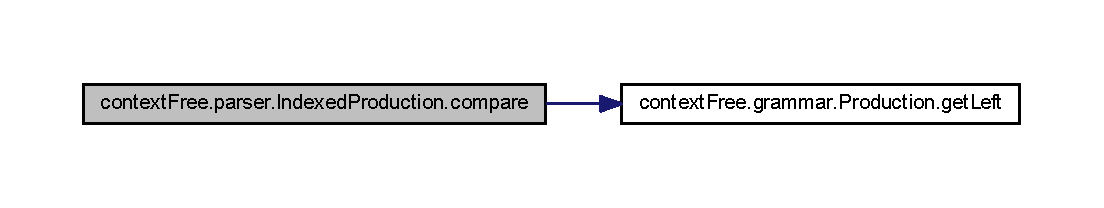
\includegraphics[width=350pt]{classcontext_free_1_1parser_1_1_indexed_production_aa79a2e2cbbc1f35d6416647d80daf3d8_cgraph}
\end{center}
\end{figure}


\hypertarget{classcontext_free_1_1parser_1_1_indexed_production_a498db47a05e7f10e580d689e925193b4}{\index{context\-Free\-::parser\-::\-Indexed\-Production@{context\-Free\-::parser\-::\-Indexed\-Production}!get\-Char\-After@{get\-Char\-After}}
\index{get\-Char\-After@{get\-Char\-After}!contextFree::parser::IndexedProduction@{context\-Free\-::parser\-::\-Indexed\-Production}}
\subsubsection[{get\-Char\-After}]{\setlength{\rightskip}{0pt plus 5cm}String {\bf context\-Free.\-parser.\-Indexed\-Production.\-get\-Char\-After} (
\begin{DoxyParamCaption}
{}
\end{DoxyParamCaption}
)}}\label{classcontext_free_1_1parser_1_1_indexed_production_a498db47a05e7f10e580d689e925193b4}


Return the next character that that will be read. 

\begin{DoxyReturn}{Returns}
the character after dot in the production 
\end{DoxyReturn}


Definition at line 74 of file Indexed\-Production.\-java.

\hypertarget{classcontext_free_1_1parser_1_1_indexed_production_a94e0e318a96518ee50607e682e7f0382}{\index{context\-Free\-::parser\-::\-Indexed\-Production@{context\-Free\-::parser\-::\-Indexed\-Production}!get\-Lookahead@{get\-Lookahead}}
\index{get\-Lookahead@{get\-Lookahead}!contextFree::parser::IndexedProduction@{context\-Free\-::parser\-::\-Indexed\-Production}}
\subsubsection[{get\-Lookahead}]{\setlength{\rightskip}{0pt plus 5cm}Set$<$String$>$ {\bf context\-Free.\-parser.\-Indexed\-Production.\-get\-Lookahead} (
\begin{DoxyParamCaption}
{}
\end{DoxyParamCaption}
)}}\label{classcontext_free_1_1parser_1_1_indexed_production_a94e0e318a96518ee50607e682e7f0382}
\begin{DoxyReturn}{Returns}
a reference to the lookahead list 
\end{DoxyReturn}


Definition at line 99 of file Indexed\-Production.\-java.



Here is the caller graph for this function\-:
\nopagebreak
\begin{figure}[H]
\begin{center}
\leavevmode
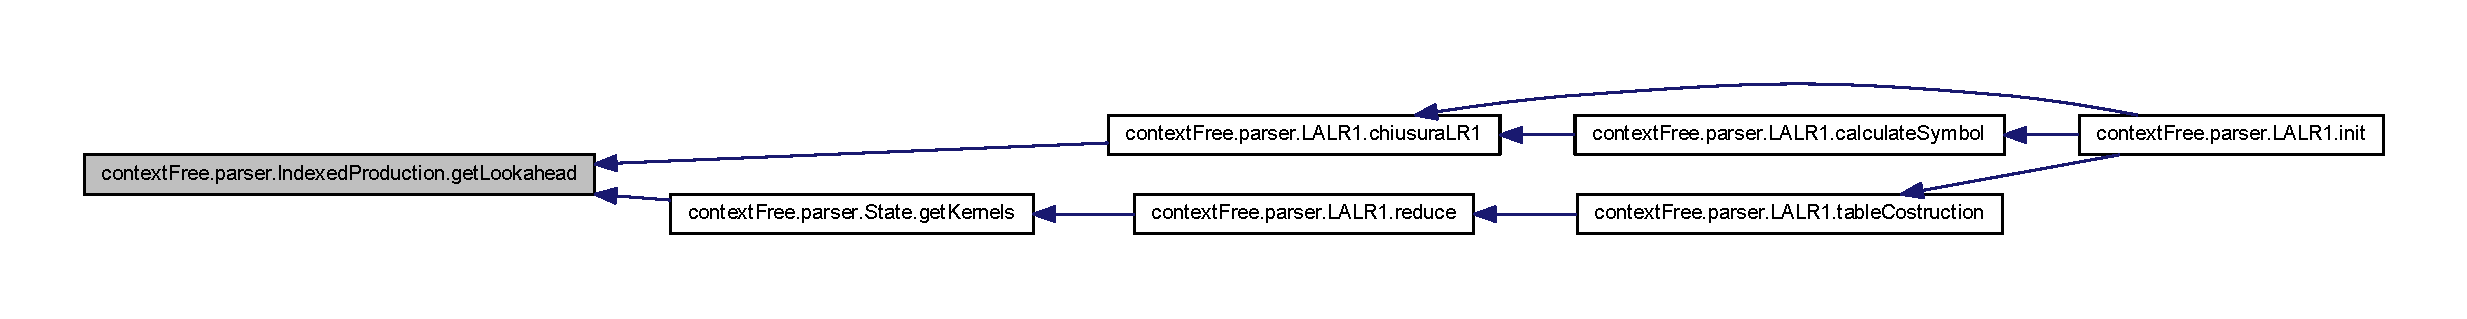
\includegraphics[width=350pt]{classcontext_free_1_1parser_1_1_indexed_production_a94e0e318a96518ee50607e682e7f0382_icgraph}
\end{center}
\end{figure}




The documentation for this class was generated from the following file\-:\begin{DoxyCompactItemize}
\item 
src/context\-Free/parser/Indexed\-Production.\-java\end{DoxyCompactItemize}

\hypertarget{classinput_parser_1_1_input_parser}{\section{input\-Parser.\-Input\-Parser Class Reference}
\label{classinput_parser_1_1_input_parser}\index{input\-Parser.\-Input\-Parser@{input\-Parser.\-Input\-Parser}}
}
Inheritance diagram for input\-Parser.\-Input\-Parser\-:\begin{figure}[H]
\begin{center}
\leavevmode
\includegraphics[height=1.314554cm]{classinput_parser_1_1_input_parser}
\end{center}
\end{figure}
\subsection*{Public Member Functions}
\begin{DoxyCompactItemize}
\item 
abstract Object \hyperlink{classinput_parser_1_1_input_parser_ab00c1fa5b5476e62889347018764fe96}{parse} ()  throws Exception
\end{DoxyCompactItemize}


\subsection{Detailed Description}


Definition at line 3 of file Input\-Parser.\-java.



\subsection{Member Function Documentation}
\hypertarget{classinput_parser_1_1_input_parser_ab00c1fa5b5476e62889347018764fe96}{\index{input\-Parser\-::\-Input\-Parser@{input\-Parser\-::\-Input\-Parser}!parse@{parse}}
\index{parse@{parse}!inputParser::InputParser@{input\-Parser\-::\-Input\-Parser}}
\subsubsection[{parse}]{\setlength{\rightskip}{0pt plus 5cm}abstract Object {\bf input\-Parser.\-Input\-Parser.\-parse} (
\begin{DoxyParamCaption}
{}
\end{DoxyParamCaption}
)  throws Exception\hspace{0.3cm}{\ttfamily  \mbox{[}pure virtual\mbox{]}}}}\label{classinput_parser_1_1_input_parser_ab00c1fa5b5476e62889347018764fe96}


Implemented in \hyperlink{classinput_parser_1_1_four_line_input_parser_a99c37488d66cfeecb33e13d573b4a81a}{input\-Parser.\-Four\-Line\-Input\-Parser}, \hyperlink{classinput_parser_1_1_single_line_input_parser_ad822676b0d3182a591e2004c3bcc79d5}{input\-Parser.\-Single\-Line\-Input\-Parser}, \hyperlink{classinput_parser_1_1_grammar_parser_a46c33fdad541b475abc31e44d56eb507}{input\-Parser.\-Grammar\-Parser}, and \hyperlink{classinput_parser_1_1_l_r_input_parser_ab1fb2966ece506eead96dcededca86a6}{input\-Parser.\-L\-R\-Input\-Parser}.



The documentation for this class was generated from the following file\-:\begin{DoxyCompactItemize}
\item 
src/input\-Parser/\hyperlink{_input_parser_8java}{Input\-Parser.\-java}\end{DoxyCompactItemize}

\hypertarget{classinput_parser_1_1_input_parser_factory}{\section{input\-Parser.\-Input\-Parser\-Factory Class Reference}
\label{classinput_parser_1_1_input_parser_factory}\index{input\-Parser.\-Input\-Parser\-Factory@{input\-Parser.\-Input\-Parser\-Factory}}
}


Inheritance diagram for input\-Parser.\-Input\-Parser\-Factory\-:
\subsection*{Protected Member Functions}
\begin{DoxyCompactItemize}
\item 
\hypertarget{classinput_parser_1_1_input_parser_factory_a48971c2679b589f34a7051e795d48c49}{abstract \hyperlink{classinput_parser_1_1_abstract_input_parser}{Abstract\-Input\-Parser} {\bfseries factory\-Method} (String in)}\label{classinput_parser_1_1_input_parser_factory_a48971c2679b589f34a7051e795d48c49}

\end{DoxyCompactItemize}


\subsection{Detailed Description}


Definition at line 3 of file Input\-Parser\-Factory.\-java.



The documentation for this class was generated from the following file\-:\begin{DoxyCompactItemize}
\item 
src/input\-Parser/Input\-Parser\-Factory.\-java\end{DoxyCompactItemize}

\hypertarget{interfacecontext_free_1_1parser_1_1_i_parser}{\section{context\-Free.\-parser.\-I\-Parser Interface Reference}
\label{interfacecontext_free_1_1parser_1_1_i_parser}\index{context\-Free.\-parser.\-I\-Parser@{context\-Free.\-parser.\-I\-Parser}}
}


Inheritance diagram for context\-Free.\-parser.\-I\-Parser\-:
\nopagebreak
\begin{figure}[H]
\begin{center}
\leavevmode
\includegraphics[height=550pt]{interfacecontext_free_1_1parser_1_1_i_parser__inherit__graph}
\end{center}
\end{figure}
\subsection*{Public Member Functions}
\begin{DoxyCompactItemize}
\item 
\hypertarget{interfacecontext_free_1_1parser_1_1_i_parser_aa0b56b8cc9bf60ddd02d5fb6a99d16bd}{void {\bfseries set\-Grammar} (\hyperlink{interfacecontext_free_1_1grammar_1_1_i_grammar}{I\-Grammar} gram)}\label{interfacecontext_free_1_1parser_1_1_i_parser_aa0b56b8cc9bf60ddd02d5fb6a99d16bd}

\item 
\hypertarget{interfacecontext_free_1_1parser_1_1_i_parser_a26c1dede13720e51bf04464b15ce1f01}{int {\bfseries init} ()  throws Exception}\label{interfacecontext_free_1_1parser_1_1_i_parser_a26c1dede13720e51bf04464b15ce1f01}

\item 
\hypertarget{interfacecontext_free_1_1parser_1_1_i_parser_a19a6f39c3ebc05c90845096a2b1c5889}{\hyperlink{interfacecontext_free_1_1grammar_1_1_i_grammar}{I\-Grammar} {\bfseries get\-Grammar} ()}\label{interfacecontext_free_1_1parser_1_1_i_parser_a19a6f39c3ebc05c90845096a2b1c5889}

\item 
\hypertarget{interfacecontext_free_1_1parser_1_1_i_parser_a29c662e040f218bfba40fb3e8c394615}{boolean {\bfseries is\-Ambiguos} ()}\label{interfacecontext_free_1_1parser_1_1_i_parser_a29c662e040f218bfba40fb3e8c394615}

\item 
\hypertarget{interfacecontext_free_1_1parser_1_1_i_parser_ad977787bef5bdc14b422945143a0414c}{\hyperlink{classcontext_free_1_1parser_1_1_automa}{Automa} {\bfseries get\-Automa} ()}\label{interfacecontext_free_1_1parser_1_1_i_parser_ad977787bef5bdc14b422945143a0414c}

\end{DoxyCompactItemize}


\subsection{Detailed Description}


Definition at line 5 of file I\-Parser.\-java.



The documentation for this interface was generated from the following file\-:\begin{DoxyCompactItemize}
\item 
src/context\-Free/parser/I\-Parser.\-java\end{DoxyCompactItemize}

\hypertarget{classcontext_free_1_1parser_1_1_l_a_l_r1}{\section{context\-Free.\-parser.\-L\-A\-L\-R1 Class Reference}
\label{classcontext_free_1_1parser_1_1_l_a_l_r1}\index{context\-Free.\-parser.\-L\-A\-L\-R1@{context\-Free.\-parser.\-L\-A\-L\-R1}}
}


Inheritance diagram for context\-Free.\-parser.\-L\-A\-L\-R1\-:
\nopagebreak
\begin{figure}[H]
\begin{center}
\leavevmode
\includegraphics[height=550pt]{classcontext_free_1_1parser_1_1_l_a_l_r1__inherit__graph}
\end{center}
\end{figure}


Collaboration diagram for context\-Free.\-parser.\-L\-A\-L\-R1\-:
\nopagebreak
\begin{figure}[H]
\begin{center}
\leavevmode
\includegraphics[width=350pt]{classcontext_free_1_1parser_1_1_l_a_l_r1__coll__graph}
\end{center}
\end{figure}
\subsection*{Public Member Functions}
\begin{DoxyCompactItemize}
\item 
\hypertarget{classcontext_free_1_1parser_1_1_l_a_l_r1_a38a0cedcd893b16f8207455f2287a7ad}{{\bfseries L\-A\-L\-R1} (\hyperlink{interfacecontext_free_1_1grammar_1_1_i_grammar}{I\-Grammar} gram)}\label{classcontext_free_1_1parser_1_1_l_a_l_r1_a38a0cedcd893b16f8207455f2287a7ad}

\item 
\hypertarget{classcontext_free_1_1parser_1_1_l_a_l_r1_a4dcd4a4ae0b77edc1dc8abffca59c80a}{String\mbox{[}$\,$\mbox{]}\mbox{[}$\,$\mbox{]} {\bfseries get\-Action\-Table} ()}\label{classcontext_free_1_1parser_1_1_l_a_l_r1_a4dcd4a4ae0b77edc1dc8abffca59c80a}

\item 
\hypertarget{classcontext_free_1_1parser_1_1_l_a_l_r1_a4bf6b83fddf359b6b0f6df26b1e58455}{void {\bfseries set\-Action\-Table} (String\mbox{[}$\,$\mbox{]}\mbox{[}$\,$\mbox{]} action\-Table)}\label{classcontext_free_1_1parser_1_1_l_a_l_r1_a4bf6b83fddf359b6b0f6df26b1e58455}

\item 
\hypertarget{classcontext_free_1_1parser_1_1_l_a_l_r1_af87607068fe2d41d8abbdb49fdeefcc0}{String\mbox{[}$\,$\mbox{]}\mbox{[}$\,$\mbox{]} {\bfseries get\-Goto\-Table} ()}\label{classcontext_free_1_1parser_1_1_l_a_l_r1_af87607068fe2d41d8abbdb49fdeefcc0}

\item 
\hypertarget{classcontext_free_1_1parser_1_1_l_a_l_r1_a002ce309af59de1951007a27d86b53b7}{void {\bfseries set\-Goto\-Table} (String\mbox{[}$\,$\mbox{]}\mbox{[}$\,$\mbox{]} goto\-Table)}\label{classcontext_free_1_1parser_1_1_l_a_l_r1_a002ce309af59de1951007a27d86b53b7}

\item 
\hypertarget{classcontext_free_1_1parser_1_1_l_a_l_r1_a27ddf376aef3ff22758c44017b37c63d}{\hyperlink{classcontext_free_1_1parser_1_1_automa}{Automa} {\bfseries get\-Automa} ()}\label{classcontext_free_1_1parser_1_1_l_a_l_r1_a27ddf376aef3ff22758c44017b37c63d}

\item 
\hypertarget{classcontext_free_1_1parser_1_1_l_a_l_r1_ab1127f78e9b15a062f6bf344f1117327}{\hyperlink{interfacecontext_free_1_1grammar_1_1_i_grammar}{I\-Grammar} {\bfseries get\-Grammar} ()}\label{classcontext_free_1_1parser_1_1_l_a_l_r1_ab1127f78e9b15a062f6bf344f1117327}

\item 
\hypertarget{classcontext_free_1_1parser_1_1_l_a_l_r1_a66f5fb1ac9aab089d3fa937acf3f63ce}{void {\bfseries set\-Grammar} (\hyperlink{interfacecontext_free_1_1grammar_1_1_i_grammar}{I\-Grammar} gram)}\label{classcontext_free_1_1parser_1_1_l_a_l_r1_a66f5fb1ac9aab089d3fa937acf3f63ce}

\item 
int \hyperlink{classcontext_free_1_1parser_1_1_l_a_l_r1_a7618cff4af4edfffb9a538a7cb1e79cf}{init} ()  throws Exception
\begin{DoxyCompactList}\small\item\em Initialize the L\-A\-L\-R(1) automaton from \hyperlink{classcontext_free_1_1parser_1_1_l_r0}{L\-R0} automaton. \end{DoxyCompactList}\item 
List$<$ \hyperlink{classcontext_free_1_1parser_1_1_indexed_production}{Indexed\-Production} $>$ \hyperlink{classcontext_free_1_1parser_1_1_l_a_l_r1_ac711dbbc2be25d15c1a8aade7579e94e}{chiusura\-L\-R1} (List$<$ \hyperlink{classcontext_free_1_1parser_1_1_indexed_production}{Indexed\-Production} $>$ i)
\begin{DoxyCompactList}\small\item\em Passed a list of production I that form the kernel of a state, return closing it, and the lookahead symbols associated. \end{DoxyCompactList}\item 
int \hyperlink{classcontext_free_1_1parser_1_1_l_a_l_r1_a79576626b3b59b832faecc986b293b36}{table\-Costruction} ()  throws Exception
\begin{DoxyCompactList}\small\item\em builds the Action table Go\-To from an automa \hyperlink{classcontext_free_1_1parser_1_1_l_a_l_r1}{L\-A\-L\-R1} and tells us if it is or not type of \hyperlink{classcontext_free_1_1parser_1_1_l_a_l_r1}{L\-A\-L\-R1} \end{DoxyCompactList}\item 
boolean \hyperlink{classcontext_free_1_1parser_1_1_l_a_l_r1_a2281981b3043c0150c1b3d3967572b1f}{reduce} (\hyperlink{classcontext_free_1_1parser_1_1_state}{State} stato)
\begin{DoxyCompactList}\small\item\em if the point is in the last position he wrote the reduces in the action table. \end{DoxyCompactList}\item 
boolean \hyperlink{classcontext_free_1_1parser_1_1_l_a_l_r1_a7379103379c94e377daca0022b28771e}{action\-Write} (int i, int j, int x, String action)
\begin{DoxyCompactList}\small\item\em Writes the action Reduce or Scift in the Action table. \end{DoxyCompactList}\item 
\hypertarget{classcontext_free_1_1parser_1_1_l_a_l_r1_a9c19be71fc16e04343eb3c23b6eac9da}{boolean {\bfseries is\-Ambiguos} ()}\label{classcontext_free_1_1parser_1_1_l_a_l_r1_a9c19be71fc16e04343eb3c23b6eac9da}

\item 
String \hyperlink{classcontext_free_1_1parser_1_1_l_a_l_r1_ad7628eb817b4a8efff71f6e22cc1659f}{print\-Table} ()
\begin{DoxyCompactList}\small\item\em Return a string with tables Goto Action. \end{DoxyCompactList}\item 
\hypertarget{classcontext_free_1_1parser_1_1_l_a_l_r1_afa3cc07b08ecbe69486105beb311eb69}{String {\bfseries to\-String} ()}\label{classcontext_free_1_1parser_1_1_l_a_l_r1_afa3cc07b08ecbe69486105beb311eb69}

\end{DoxyCompactItemize}
\subsection*{Static Package Attributes}
\begin{DoxyCompactItemize}
\item 
\hypertarget{classcontext_free_1_1parser_1_1_l_a_l_r1_a9684757c9b143a5b82609c1de472400e}{static Logger {\bfseries logger} = Logger.\-get\-Logger(L\-A\-L\-R1.\-class.\-get\-Name())}\label{classcontext_free_1_1parser_1_1_l_a_l_r1_a9684757c9b143a5b82609c1de472400e}

\end{DoxyCompactItemize}
\subsection*{Private Member Functions}
\begin{DoxyCompactItemize}
\item 
int \hyperlink{classcontext_free_1_1parser_1_1_l_a_l_r1_aeec32b5c83e031225114f46ac377f804}{calculate\-Symbol} (\hyperlink{classcontext_free_1_1parser_1_1_automa}{Automa} atm)  throws Exception
\begin{DoxyCompactList}\small\item\em Calculate one step of lookahead symbol from an automaton with the algorithm of spontaneous generation and propagation of symbol. \end{DoxyCompactList}\end{DoxyCompactItemize}
\subsection*{Private Attributes}
\begin{DoxyCompactItemize}
\item 
\hypertarget{classcontext_free_1_1parser_1_1_l_a_l_r1_a3e69dd16d8b89cc9a210286efe0aa0d8}{boolean {\bfseries is\-Ambiguous} = false}\label{classcontext_free_1_1parser_1_1_l_a_l_r1_a3e69dd16d8b89cc9a210286efe0aa0d8}

\item 
\hypertarget{classcontext_free_1_1parser_1_1_l_a_l_r1_ac76b78ae26e1f59674ae10b9c1059213}{String {\bfseries ambiguo} = \char`\"{}\char`\"{}}\label{classcontext_free_1_1parser_1_1_l_a_l_r1_ac76b78ae26e1f59674ae10b9c1059213}

\item 
\hypertarget{classcontext_free_1_1parser_1_1_l_a_l_r1_ab6054628eaec08e8b3b77a37e219ef02}{\hyperlink{classcontext_free_1_1parser_1_1_automa}{Automa} {\bfseries automa}}\label{classcontext_free_1_1parser_1_1_l_a_l_r1_ab6054628eaec08e8b3b77a37e219ef02}

\item 
\hypertarget{classcontext_free_1_1parser_1_1_l_a_l_r1_a50a59810900d20102a28766aad917b79}{String\mbox{[}$\,$\mbox{]}\mbox{[}$\,$\mbox{]} {\bfseries action\-Table}}\label{classcontext_free_1_1parser_1_1_l_a_l_r1_a50a59810900d20102a28766aad917b79}

\item 
\hypertarget{classcontext_free_1_1parser_1_1_l_a_l_r1_a6f27da8ba10ef81be36845b0fffc9858}{String\mbox{[}$\,$\mbox{]}\mbox{[}$\,$\mbox{]} {\bfseries goto\-Table}}\label{classcontext_free_1_1parser_1_1_l_a_l_r1_a6f27da8ba10ef81be36845b0fffc9858}

\end{DoxyCompactItemize}


\subsection{Detailed Description}


Definition at line 14 of file L\-A\-L\-R1.\-java.



\subsection{Member Function Documentation}
\hypertarget{classcontext_free_1_1parser_1_1_l_a_l_r1_a7379103379c94e377daca0022b28771e}{\index{context\-Free\-::parser\-::\-L\-A\-L\-R1@{context\-Free\-::parser\-::\-L\-A\-L\-R1}!action\-Write@{action\-Write}}
\index{action\-Write@{action\-Write}!contextFree::parser::LALR1@{context\-Free\-::parser\-::\-L\-A\-L\-R1}}
\subsubsection[{action\-Write}]{\setlength{\rightskip}{0pt plus 5cm}boolean {\bf context\-Free.\-parser.\-L\-A\-L\-R1.\-action\-Write} (
\begin{DoxyParamCaption}
\item[{int}]{i, }
\item[{int}]{j, }
\item[{int}]{x, }
\item[{String}]{action}
\end{DoxyParamCaption}
)}}\label{classcontext_free_1_1parser_1_1_l_a_l_r1_a7379103379c94e377daca0022b28771e}


Writes the action Reduce or Scift in the Action table. 


\begin{DoxyParams}{Parameters}
{\em current} & state \\
\hline
{\em -\/1} & If it reduces, else the destination state of the shift \\
\hline
{\em symbol} & for which you go write in the Action table \\
\hline
{\em action} & \char`\"{}s\char`\"{} if it is shift, else the production for which reduce \\
\hline
\end{DoxyParams}
\begin{DoxyReturn}{Returns}
false case of ambiguity 
\end{DoxyReturn}
\begin{DoxyAuthor}{Author}
Pierluigi Sottile 
\end{DoxyAuthor}


Definition at line 369 of file L\-A\-L\-R1.\-java.



Here is the caller graph for this function\-:
\nopagebreak
\begin{figure}[H]
\begin{center}
\leavevmode
\includegraphics[width=350pt]{classcontext_free_1_1parser_1_1_l_a_l_r1_a7379103379c94e377daca0022b28771e_icgraph}
\end{center}
\end{figure}


\hypertarget{classcontext_free_1_1parser_1_1_l_a_l_r1_aeec32b5c83e031225114f46ac377f804}{\index{context\-Free\-::parser\-::\-L\-A\-L\-R1@{context\-Free\-::parser\-::\-L\-A\-L\-R1}!calculate\-Symbol@{calculate\-Symbol}}
\index{calculate\-Symbol@{calculate\-Symbol}!contextFree::parser::LALR1@{context\-Free\-::parser\-::\-L\-A\-L\-R1}}
\subsubsection[{calculate\-Symbol}]{\setlength{\rightskip}{0pt plus 5cm}int {\bf context\-Free.\-parser.\-L\-A\-L\-R1.\-calculate\-Symbol} (
\begin{DoxyParamCaption}
\item[{{\bf Automa}}]{atm}
\end{DoxyParamCaption}
)  throws Exception\hspace{0.3cm}{\ttfamily  \mbox{[}private\mbox{]}}}}\label{classcontext_free_1_1parser_1_1_l_a_l_r1_aeec32b5c83e031225114f46ac377f804}


Calculate one step of lookahead symbol from an automaton with the algorithm of spontaneous generation and propagation of symbol. 


\begin{DoxyParams}{Parameters}
{\em atm} & the automaton \\
\hline
\end{DoxyParams}
\begin{DoxyReturn}{Returns}
0 if no symbol have created, 1 otherwise. -\/1 if error. 
\end{DoxyReturn}

\begin{DoxyExceptions}{Exceptions}
{\em Exception} & \\
\hline
\end{DoxyExceptions}
\begin{DoxyAuthor}{Author}
Paolo Pino 
\end{DoxyAuthor}
Trasformo la singola produzione k in una list per poterla passare a chiusura \hyperlink{classcontext_free_1_1parser_1_1_l_r1}{L\-R1} 

Definition at line 122 of file L\-A\-L\-R1.\-java.



Here is the call graph for this function\-:
\nopagebreak
\begin{figure}[H]
\begin{center}
\leavevmode
\includegraphics[width=350pt]{classcontext_free_1_1parser_1_1_l_a_l_r1_aeec32b5c83e031225114f46ac377f804_cgraph}
\end{center}
\end{figure}




Here is the caller graph for this function\-:
\nopagebreak
\begin{figure}[H]
\begin{center}
\leavevmode
\includegraphics[width=350pt]{classcontext_free_1_1parser_1_1_l_a_l_r1_aeec32b5c83e031225114f46ac377f804_icgraph}
\end{center}
\end{figure}


\hypertarget{classcontext_free_1_1parser_1_1_l_a_l_r1_ac711dbbc2be25d15c1a8aade7579e94e}{\index{context\-Free\-::parser\-::\-L\-A\-L\-R1@{context\-Free\-::parser\-::\-L\-A\-L\-R1}!chiusura\-L\-R1@{chiusura\-L\-R1}}
\index{chiusura\-L\-R1@{chiusura\-L\-R1}!contextFree::parser::LALR1@{context\-Free\-::parser\-::\-L\-A\-L\-R1}}
\subsubsection[{chiusura\-L\-R1}]{\setlength{\rightskip}{0pt plus 5cm}List$<${\bf Indexed\-Production}$>$ {\bf context\-Free.\-parser.\-L\-A\-L\-R1.\-chiusura\-L\-R1} (
\begin{DoxyParamCaption}
\item[{List$<$ {\bf Indexed\-Production} $>$}]{i}
\end{DoxyParamCaption}
)}}\label{classcontext_free_1_1parser_1_1_l_a_l_r1_ac711dbbc2be25d15c1a8aade7579e94e}


Passed a list of production I that form the kernel of a state, return closing it, and the lookahead symbols associated. 


\begin{DoxyParams}{Parameters}
{\em the} & kernels of the state \\
\hline
\end{DoxyParams}
\begin{DoxyReturn}{Returns}
list of products forming the state 
\end{DoxyReturn}
\begin{DoxyAuthor}{Author}
Pierluigi Sottile 
\end{DoxyAuthor}


Definition at line 171 of file L\-A\-L\-R1.\-java.



Here is the call graph for this function\-:
\nopagebreak
\begin{figure}[H]
\begin{center}
\leavevmode
\includegraphics[width=350pt]{classcontext_free_1_1parser_1_1_l_a_l_r1_ac711dbbc2be25d15c1a8aade7579e94e_cgraph}
\end{center}
\end{figure}




Here is the caller graph for this function\-:
\nopagebreak
\begin{figure}[H]
\begin{center}
\leavevmode
\includegraphics[width=350pt]{classcontext_free_1_1parser_1_1_l_a_l_r1_ac711dbbc2be25d15c1a8aade7579e94e_icgraph}
\end{center}
\end{figure}


\hypertarget{classcontext_free_1_1parser_1_1_l_a_l_r1_a7618cff4af4edfffb9a538a7cb1e79cf}{\index{context\-Free\-::parser\-::\-L\-A\-L\-R1@{context\-Free\-::parser\-::\-L\-A\-L\-R1}!init@{init}}
\index{init@{init}!contextFree::parser::LALR1@{context\-Free\-::parser\-::\-L\-A\-L\-R1}}
\subsubsection[{init}]{\setlength{\rightskip}{0pt plus 5cm}int {\bf context\-Free.\-parser.\-L\-A\-L\-R1.\-init} (
\begin{DoxyParamCaption}
{}
\end{DoxyParamCaption}
)  throws Exception\hspace{0.3cm}{\ttfamily  \mbox{[}virtual\mbox{]}}}}\label{classcontext_free_1_1parser_1_1_l_a_l_r1_a7618cff4af4edfffb9a538a7cb1e79cf}


Initialize the L\-A\-L\-R(1) automaton from \hyperlink{classcontext_free_1_1parser_1_1_l_r0}{L\-R0} automaton. 

If the grammar is L\-A\-L\-R(1) then initialize action and goto table. \begin{DoxyReturn}{Returns}
0 if the grammar is ambiguous, 1 otherwise. -\/1 if error 
\end{DoxyReturn}


Implements \hyperlink{classcontext_free_1_1parser_1_1_l_r0}{context\-Free.\-parser.\-L\-R0}.



Definition at line 76 of file L\-A\-L\-R1.\-java.



Here is the call graph for this function\-:
\nopagebreak
\begin{figure}[H]
\begin{center}
\leavevmode
\includegraphics[width=350pt]{classcontext_free_1_1parser_1_1_l_a_l_r1_a7618cff4af4edfffb9a538a7cb1e79cf_cgraph}
\end{center}
\end{figure}


\hypertarget{classcontext_free_1_1parser_1_1_l_a_l_r1_ad7628eb817b4a8efff71f6e22cc1659f}{\index{context\-Free\-::parser\-::\-L\-A\-L\-R1@{context\-Free\-::parser\-::\-L\-A\-L\-R1}!print\-Table@{print\-Table}}
\index{print\-Table@{print\-Table}!contextFree::parser::LALR1@{context\-Free\-::parser\-::\-L\-A\-L\-R1}}
\subsubsection[{print\-Table}]{\setlength{\rightskip}{0pt plus 5cm}String {\bf context\-Free.\-parser.\-L\-A\-L\-R1.\-print\-Table} (
\begin{DoxyParamCaption}
{}
\end{DoxyParamCaption}
)}}\label{classcontext_free_1_1parser_1_1_l_a_l_r1_ad7628eb817b4a8efff71f6e22cc1659f}


Return a string with tables Goto Action. 

\begin{DoxyReturn}{Returns}

\end{DoxyReturn}


Definition at line 401 of file L\-A\-L\-R1.\-java.



Here is the call graph for this function\-:
\nopagebreak
\begin{figure}[H]
\begin{center}
\leavevmode
\includegraphics[width=350pt]{classcontext_free_1_1parser_1_1_l_a_l_r1_ad7628eb817b4a8efff71f6e22cc1659f_cgraph}
\end{center}
\end{figure}


\hypertarget{classcontext_free_1_1parser_1_1_l_a_l_r1_a2281981b3043c0150c1b3d3967572b1f}{\index{context\-Free\-::parser\-::\-L\-A\-L\-R1@{context\-Free\-::parser\-::\-L\-A\-L\-R1}!reduce@{reduce}}
\index{reduce@{reduce}!contextFree::parser::LALR1@{context\-Free\-::parser\-::\-L\-A\-L\-R1}}
\subsubsection[{reduce}]{\setlength{\rightskip}{0pt plus 5cm}boolean {\bf context\-Free.\-parser.\-L\-A\-L\-R1.\-reduce} (
\begin{DoxyParamCaption}
\item[{{\bf State}}]{stato}
\end{DoxyParamCaption}
)}}\label{classcontext_free_1_1parser_1_1_l_a_l_r1_a2281981b3043c0150c1b3d3967572b1f}


if the point is in the last position he wrote the reduces in the action table. 


\begin{DoxyParams}{Parameters}
{\em state} & to control \\
\hline
\end{DoxyParams}
\begin{DoxyReturn}{Returns}
false if there are conflicts 
\end{DoxyReturn}
\begin{DoxyAuthor}{Author}
Pierluigi Sottile 
\end{DoxyAuthor}


Definition at line 331 of file L\-A\-L\-R1.\-java.



Here is the call graph for this function\-:
\nopagebreak
\begin{figure}[H]
\begin{center}
\leavevmode
\includegraphics[width=350pt]{classcontext_free_1_1parser_1_1_l_a_l_r1_a2281981b3043c0150c1b3d3967572b1f_cgraph}
\end{center}
\end{figure}




Here is the caller graph for this function\-:
\nopagebreak
\begin{figure}[H]
\begin{center}
\leavevmode
\includegraphics[width=350pt]{classcontext_free_1_1parser_1_1_l_a_l_r1_a2281981b3043c0150c1b3d3967572b1f_icgraph}
\end{center}
\end{figure}


\hypertarget{classcontext_free_1_1parser_1_1_l_a_l_r1_a79576626b3b59b832faecc986b293b36}{\index{context\-Free\-::parser\-::\-L\-A\-L\-R1@{context\-Free\-::parser\-::\-L\-A\-L\-R1}!table\-Costruction@{table\-Costruction}}
\index{table\-Costruction@{table\-Costruction}!contextFree::parser::LALR1@{context\-Free\-::parser\-::\-L\-A\-L\-R1}}
\subsubsection[{table\-Costruction}]{\setlength{\rightskip}{0pt plus 5cm}int {\bf context\-Free.\-parser.\-L\-A\-L\-R1.\-table\-Costruction} (
\begin{DoxyParamCaption}
{}
\end{DoxyParamCaption}
)  throws Exception}}\label{classcontext_free_1_1parser_1_1_l_a_l_r1_a79576626b3b59b832faecc986b293b36}


builds the Action table Go\-To from an automa \hyperlink{classcontext_free_1_1parser_1_1_l_a_l_r1}{L\-A\-L\-R1} and tells us if it is or not type of \hyperlink{classcontext_free_1_1parser_1_1_l_a_l_r1}{L\-A\-L\-R1} 


\begin{DoxyParams}{Parameters}
{\em automa} & to control \\
\hline
\end{DoxyParams}
\begin{DoxyReturn}{Returns}
1 if the type of grammar is L\-A\-L\-R (1), 0 otherwise 
\end{DoxyReturn}

\begin{DoxyExceptions}{Exceptions}
{\em Exception} & \\
\hline
\end{DoxyExceptions}
\begin{DoxyAuthor}{Author}
Pierluigi Sottile 
\end{DoxyAuthor}


Definition at line 280 of file L\-A\-L\-R1.\-java.



Here is the call graph for this function\-:
\nopagebreak
\begin{figure}[H]
\begin{center}
\leavevmode
\includegraphics[width=350pt]{classcontext_free_1_1parser_1_1_l_a_l_r1_a79576626b3b59b832faecc986b293b36_cgraph}
\end{center}
\end{figure}




Here is the caller graph for this function\-:
\nopagebreak
\begin{figure}[H]
\begin{center}
\leavevmode
\includegraphics[width=350pt]{classcontext_free_1_1parser_1_1_l_a_l_r1_a79576626b3b59b832faecc986b293b36_icgraph}
\end{center}
\end{figure}




The documentation for this class was generated from the following file\-:\begin{DoxyCompactItemize}
\item 
src/context\-Free/parser/L\-A\-L\-R1.\-java\end{DoxyCompactItemize}

\hypertarget{classcontext_free_1_1parser_1_1_l_r0}{\section{context\-Free.\-parser.\-L\-R0 Class Reference}
\label{classcontext_free_1_1parser_1_1_l_r0}\index{context\-Free.\-parser.\-L\-R0@{context\-Free.\-parser.\-L\-R0}}
}


Inheritance diagram for context\-Free.\-parser.\-L\-R0\-:


Collaboration diagram for context\-Free.\-parser.\-L\-R0\-:
\subsection*{Public Member Functions}
\begin{DoxyCompactItemize}
\item 
\hypertarget{classcontext_free_1_1parser_1_1_l_r0_ab87079bb387c26bad40d3678e80eefc9}{abstract void {\bfseries set\-Grammar} (\hyperlink{interfacecontext_free_1_1grammar_1_1_i_grammar}{I\-Grammar} gram)}\label{classcontext_free_1_1parser_1_1_l_r0_ab87079bb387c26bad40d3678e80eefc9}

\item 
\hypertarget{classcontext_free_1_1parser_1_1_l_r0_a1936c0d9c7c80de80a5b3913f8f710b7}{abstract int {\bfseries init} ()  throws Exception}\label{classcontext_free_1_1parser_1_1_l_r0_a1936c0d9c7c80de80a5b3913f8f710b7}

\item 
List$<$ \hyperlink{classcontext_free_1_1parser_1_1_indexed_production}{Indexed\-Production} $>$ \hyperlink{classcontext_free_1_1parser_1_1_l_r0_aa0e8369b6e2db7489437ad8a6f217d22}{chiusura} (List$<$ \hyperlink{classcontext_free_1_1parser_1_1_indexed_production}{Indexed\-Production} $>$ i)
\begin{DoxyCompactList}\small\item\em $\ast$\-I passed a list of production that form the kernel of a state, return closing it \end{DoxyCompactList}\item 
List$<$ \hyperlink{classcontext_free_1_1parser_1_1_indexed_production}{Indexed\-Production} $>$ \hyperlink{classcontext_free_1_1parser_1_1_l_r0_aea1ecb06a1880a8bc5eeb4efcca0ecea}{Go\-To} (List$<$ \hyperlink{classcontext_free_1_1parser_1_1_indexed_production}{Indexed\-Production} $>$ i, String X)
\begin{DoxyCompactList}\small\item\em Passed a state and the symbol that follows the point, returns the kernel of the new state with the relative closure. \end{DoxyCompactList}\item 
List$<$ \hyperlink{classcontext_free_1_1parser_1_1_state}{State} $>$ \hyperlink{classcontext_free_1_1parser_1_1_l_r0_aa96d752420b690ccbbc9fad67691f36a}{Item} ()
\begin{DoxyCompactList}\small\item\em given a grammar G we calculate the associated grammar augmented by adding the production S '\-:\-: =. \end{DoxyCompactList}\item 
int \hyperlink{classcontext_free_1_1parser_1_1_l_r0_a8de929e041a5a1a273e6ddd05dc7e0ca}{uguale} (List$<$ \hyperlink{classcontext_free_1_1parser_1_1_state}{State} $>$ automa, List$<$ \hyperlink{classcontext_free_1_1parser_1_1_indexed_production}{Indexed\-Production} $>$ stato)
\begin{DoxyCompactList}\small\item\em checks if a state is present in an automaton \end{DoxyCompactList}\item 
boolean \hyperlink{classcontext_free_1_1parser_1_1_l_r0_a242530010547a830ad1b9c35a724a7e6}{prod\-Presente} (List$<$ \hyperlink{classcontext_free_1_1parser_1_1_indexed_production}{Indexed\-Production} $>$j, \hyperlink{classcontext_free_1_1grammar_1_1_production}{Production} corrente)
\begin{DoxyCompactList}\small\item\em checks if a production is already in a list of productions. \end{DoxyCompactList}\end{DoxyCompactItemize}
\subsection*{Protected Attributes}
\begin{DoxyCompactItemize}
\item 
\hypertarget{classcontext_free_1_1parser_1_1_l_r0_aa81cb7c5781fa4b6f1a129077a4da618}{\hyperlink{interfacecontext_free_1_1grammar_1_1_i_grammar}{I\-Grammar} {\bfseries grammatica}}\label{classcontext_free_1_1parser_1_1_l_r0_aa81cb7c5781fa4b6f1a129077a4da618}

\end{DoxyCompactItemize}


\subsection{Detailed Description}


Definition at line 13 of file L\-R0.\-java.



\subsection{Member Function Documentation}
\hypertarget{classcontext_free_1_1parser_1_1_l_r0_aa0e8369b6e2db7489437ad8a6f217d22}{\index{context\-Free\-::parser\-::\-L\-R0@{context\-Free\-::parser\-::\-L\-R0}!chiusura@{chiusura}}
\index{chiusura@{chiusura}!contextFree::parser::LR0@{context\-Free\-::parser\-::\-L\-R0}}
\subsubsection[{chiusura}]{\setlength{\rightskip}{0pt plus 5cm}List$<${\bf Indexed\-Production}$>$ {\bf context\-Free.\-parser.\-L\-R0.\-chiusura} (
\begin{DoxyParamCaption}
\item[{List$<$ {\bf Indexed\-Production} $>$}]{i}
\end{DoxyParamCaption}
)}}\label{classcontext_free_1_1parser_1_1_l_r0_aa0e8369b6e2db7489437ad8a6f217d22}


$\ast$\-I passed a list of production that form the kernel of a state, return closing it 


\begin{DoxyParams}{Parameters}
{\em the} & kernels of the state \\
\hline
\end{DoxyParams}
\begin{DoxyReturn}{Returns}
list of products forming the state 
\end{DoxyReturn}
\begin{DoxyAuthor}{Author}
Pierluigi Sottile 
\end{DoxyAuthor}


Definition at line 27 of file L\-R0.\-java.



Here is the call graph for this function\-:




Here is the caller graph for this function\-:


\hypertarget{classcontext_free_1_1parser_1_1_l_r0_aea1ecb06a1880a8bc5eeb4efcca0ecea}{\index{context\-Free\-::parser\-::\-L\-R0@{context\-Free\-::parser\-::\-L\-R0}!Go\-To@{Go\-To}}
\index{Go\-To@{Go\-To}!contextFree::parser::LR0@{context\-Free\-::parser\-::\-L\-R0}}
\subsubsection[{Go\-To}]{\setlength{\rightskip}{0pt plus 5cm}List$<${\bf Indexed\-Production}$>$ {\bf context\-Free.\-parser.\-L\-R0.\-Go\-To} (
\begin{DoxyParamCaption}
\item[{List$<$ {\bf Indexed\-Production} $>$}]{i, }
\item[{String}]{X}
\end{DoxyParamCaption}
)}}\label{classcontext_free_1_1parser_1_1_l_r0_aea1ecb06a1880a8bc5eeb4efcca0ecea}


Passed a state and the symbol that follows the point, returns the kernel of the new state with the relative closure. 


\begin{DoxyParams}{Parameters}
{\em \hyperlink{classcontext_free_1_1parser_1_1_state}{State}} & which calculated to be the new kernel \\
\hline
{\em X} & symbol that moves the point \\
\hline
\end{DoxyParams}
\begin{DoxyReturn}{Returns}
closure of new state 
\end{DoxyReturn}
\begin{DoxyAuthor}{Author}
Pierluigi Sottile 
\end{DoxyAuthor}


Definition at line 89 of file L\-R0.\-java.



Here is the call graph for this function\-:




Here is the caller graph for this function\-:


\hypertarget{classcontext_free_1_1parser_1_1_l_r0_aa96d752420b690ccbbc9fad67691f36a}{\index{context\-Free\-::parser\-::\-L\-R0@{context\-Free\-::parser\-::\-L\-R0}!Item@{Item}}
\index{Item@{Item}!contextFree::parser::LR0@{context\-Free\-::parser\-::\-L\-R0}}
\subsubsection[{Item}]{\setlength{\rightskip}{0pt plus 5cm}List$<${\bf State}$>$ {\bf context\-Free.\-parser.\-L\-R0.\-Item} (
\begin{DoxyParamCaption}
{}
\end{DoxyParamCaption}
)}}\label{classcontext_free_1_1parser_1_1_l_r0_aa96d752420b690ccbbc9fad67691f36a}


given a grammar G we calculate the associated grammar augmented by adding the production S '\-:\-: =. 

S, where S is the assiom. We calculate the closure of it and so associated Go\-To 'to have the finite state autom. \begin{DoxyReturn}{Returns}
the autom L\-R(0) 
\end{DoxyReturn}
\begin{DoxyAuthor}{Author}
Pierluigi Sottile 
\end{DoxyAuthor}


Definition at line 118 of file L\-R0.\-java.



Here is the call graph for this function\-:




Here is the caller graph for this function\-:


\hypertarget{classcontext_free_1_1parser_1_1_l_r0_a242530010547a830ad1b9c35a724a7e6}{\index{context\-Free\-::parser\-::\-L\-R0@{context\-Free\-::parser\-::\-L\-R0}!prod\-Presente@{prod\-Presente}}
\index{prod\-Presente@{prod\-Presente}!contextFree::parser::LR0@{context\-Free\-::parser\-::\-L\-R0}}
\subsubsection[{prod\-Presente}]{\setlength{\rightskip}{0pt plus 5cm}boolean {\bf context\-Free.\-parser.\-L\-R0.\-prod\-Presente} (
\begin{DoxyParamCaption}
\item[{List$<$ {\bf Indexed\-Production} $>$}]{j, }
\item[{{\bf Production}}]{corrente}
\end{DoxyParamCaption}
)}}\label{classcontext_free_1_1parser_1_1_l_r0_a242530010547a830ad1b9c35a724a7e6}


checks if a production is already in a list of productions. 


\begin{DoxyParams}{Parameters}
{\em the} & state in which control \\
\hline
{\em prodaction} & to search \\
\hline
\end{DoxyParams}
\begin{DoxyReturn}{Returns}
true if there is false if it is not 
\end{DoxyReturn}
\begin{DoxyAuthor}{Author}
Pierluigi Sottile 
\end{DoxyAuthor}


Definition at line 247 of file L\-R0.\-java.



Here is the call graph for this function\-:




Here is the caller graph for this function\-:


\hypertarget{classcontext_free_1_1parser_1_1_l_r0_a8de929e041a5a1a273e6ddd05dc7e0ca}{\index{context\-Free\-::parser\-::\-L\-R0@{context\-Free\-::parser\-::\-L\-R0}!uguale@{uguale}}
\index{uguale@{uguale}!contextFree::parser::LR0@{context\-Free\-::parser\-::\-L\-R0}}
\subsubsection[{uguale}]{\setlength{\rightskip}{0pt plus 5cm}int {\bf context\-Free.\-parser.\-L\-R0.\-uguale} (
\begin{DoxyParamCaption}
\item[{List$<$ {\bf State} $>$}]{automa, }
\item[{List$<$ {\bf Indexed\-Production} $>$}]{stato}
\end{DoxyParamCaption}
)}}\label{classcontext_free_1_1parser_1_1_l_r0_a8de929e041a5a1a273e6ddd05dc7e0ca}


checks if a state is present in an automaton 


\begin{DoxyParams}{Parameters}
{\em autom} & \\
\hline
{\em state} & to search \\
\hline
\end{DoxyParams}
\begin{DoxyReturn}{Returns}
-\/1 If not present, otherwise returns the number state equal to the past 
\end{DoxyReturn}
\begin{DoxyAuthor}{Author}
Pierluigi Sottile 
\end{DoxyAuthor}


Definition at line 198 of file L\-R0.\-java.



Here is the call graph for this function\-:




Here is the caller graph for this function\-:




The documentation for this class was generated from the following file\-:\begin{DoxyCompactItemize}
\item 
src/context\-Free/parser/L\-R0.\-java\end{DoxyCompactItemize}

\hypertarget{classcontext_free_1_1parser_1_1_l_r1}{\section{context\-Free.\-parser.\-L\-R1 Class Reference}
\label{classcontext_free_1_1parser_1_1_l_r1}\index{context\-Free.\-parser.\-L\-R1@{context\-Free.\-parser.\-L\-R1}}
}


Collaboration diagram for context\-Free.\-parser.\-L\-R1\-:\nopagebreak
\begin{figure}[H]
\begin{center}
\leavevmode
\includegraphics[width=234pt]{classcontext_free_1_1parser_1_1_l_r1__coll__graph}
\end{center}
\end{figure}
\subsection*{Public Member Functions}
\begin{DoxyCompactItemize}
\item 
\hypertarget{classcontext_free_1_1parser_1_1_l_r1_a464d377de8e3484383068a547208dab5}{abstract void {\bfseries set\-Grammar} (\hyperlink{interfacecontext_free_1_1grammar_1_1_i_grammar}{I\-Grammar} gram)}\label{classcontext_free_1_1parser_1_1_l_r1_a464d377de8e3484383068a547208dab5}

\end{DoxyCompactItemize}
\subsection*{Protected Attributes}
\begin{DoxyCompactItemize}
\item 
\hypertarget{classcontext_free_1_1parser_1_1_l_r1_a1639494e6b5ede7a4e9b6e4c24fd1702}{\hyperlink{interfacecontext_free_1_1grammar_1_1_i_grammar}{I\-Grammar} {\bfseries grammatica}}\label{classcontext_free_1_1parser_1_1_l_r1_a1639494e6b5ede7a4e9b6e4c24fd1702}

\end{DoxyCompactItemize}


\subsection{Detailed Description}


Definition at line 6 of file L\-R1.\-java.



The documentation for this class was generated from the following file\-:\begin{DoxyCompactItemize}
\item 
src/context\-Free/parser/L\-R1.\-java\end{DoxyCompactItemize}

\hypertarget{classinput_parser_1_1_l_r_input_parser}{\section{input\-Parser.\-L\-R\-Input\-Parser Class Reference}
\label{classinput_parser_1_1_l_r_input_parser}\index{input\-Parser.\-L\-R\-Input\-Parser@{input\-Parser.\-L\-R\-Input\-Parser}}
}


Parse a txt file with action table, goto table and grammar in one line format ($\ast$.1l).  


Inheritance diagram for input\-Parser.\-L\-R\-Input\-Parser\-:\begin{figure}[H]
\begin{center}
\leavevmode
\includegraphics[height=2.000000cm]{classinput_parser_1_1_l_r_input_parser}
\end{center}
\end{figure}
\subsection*{Public Member Functions}
\begin{DoxyCompactItemize}
\item 
\hyperlink{classinput_parser_1_1_l_r_input_parser_a243ff5c225bbbe63bc64e615fed97ec4}{L\-R\-Input\-Parser} ()
\item 
\hyperlink{classinput_parser_1_1_l_r_input_parser_a42f9947db4e863a82e3a8ca89c655c2a}{L\-R\-Input\-Parser} (String in)
\item 
\hyperlink{classparser_program_1_1_parser}{Parser} \hyperlink{classinput_parser_1_1_l_r_input_parser_ab1fb2966ece506eead96dcededca86a6}{parse} ()  throws Exception 
\begin{DoxyCompactList}\small\item\em Parse method. \end{DoxyCompactList}\end{DoxyCompactItemize}
\subsection*{Static Package Attributes}
\begin{DoxyCompactItemize}
\item 
static Logger \hyperlink{classinput_parser_1_1_l_r_input_parser_ae3d6e07ebb7d4368f1a2e2ad05dae6f7}{logger} = Logger.\-get\-Logger(L\-R\-Input\-Parser.\-class.\-get\-Name())
\end{DoxyCompactItemize}
\subsection*{Private Member Functions}
\begin{DoxyCompactItemize}
\item 
void \hyperlink{classinput_parser_1_1_l_r_input_parser_a1ade16089652dc354434e1ddb1769e96}{read\-Table} (Buffered\-Reader f, Hashtable$<$ String, List$<$ String $>$$>$ table)  throws I\-O\-Exception 
\begin{DoxyCompactList}\small\item\em read the table in the first part of the file and store it in an hashtable with simbol as key and a list with an element for each state \end{DoxyCompactList}\end{DoxyCompactItemize}
\subsection*{Private Attributes}
\begin{DoxyCompactItemize}
\item 
String \hyperlink{classinput_parser_1_1_l_r_input_parser_a7f407afa631516efdbaf3cee992bb16f}{input}
\end{DoxyCompactItemize}


\subsection{Detailed Description}
Parse a txt file with action table, goto table and grammar in one line format ($\ast$.1l). 

\begin{DoxyAuthor}{Author}
Paolo Pino 
\end{DoxyAuthor}


Definition at line 21 of file L\-R\-Input\-Parser.\-java.



\subsection{Constructor \& Destructor Documentation}
\hypertarget{classinput_parser_1_1_l_r_input_parser_a243ff5c225bbbe63bc64e615fed97ec4}{\index{input\-Parser\-::\-L\-R\-Input\-Parser@{input\-Parser\-::\-L\-R\-Input\-Parser}!L\-R\-Input\-Parser@{L\-R\-Input\-Parser}}
\index{L\-R\-Input\-Parser@{L\-R\-Input\-Parser}!inputParser::LRInputParser@{input\-Parser\-::\-L\-R\-Input\-Parser}}
\subsubsection[{L\-R\-Input\-Parser}]{\setlength{\rightskip}{0pt plus 5cm}{\bf input\-Parser.\-L\-R\-Input\-Parser.\-L\-R\-Input\-Parser} (
\begin{DoxyParamCaption}
{}
\end{DoxyParamCaption}
)}}\label{classinput_parser_1_1_l_r_input_parser_a243ff5c225bbbe63bc64e615fed97ec4}


Definition at line 26 of file L\-R\-Input\-Parser.\-java.

\hypertarget{classinput_parser_1_1_l_r_input_parser_a42f9947db4e863a82e3a8ca89c655c2a}{\index{input\-Parser\-::\-L\-R\-Input\-Parser@{input\-Parser\-::\-L\-R\-Input\-Parser}!L\-R\-Input\-Parser@{L\-R\-Input\-Parser}}
\index{L\-R\-Input\-Parser@{L\-R\-Input\-Parser}!inputParser::LRInputParser@{input\-Parser\-::\-L\-R\-Input\-Parser}}
\subsubsection[{L\-R\-Input\-Parser}]{\setlength{\rightskip}{0pt plus 5cm}{\bf input\-Parser.\-L\-R\-Input\-Parser.\-L\-R\-Input\-Parser} (
\begin{DoxyParamCaption}
\item[{String}]{in}
\end{DoxyParamCaption}
)}}\label{classinput_parser_1_1_l_r_input_parser_a42f9947db4e863a82e3a8ca89c655c2a}


Definition at line 29 of file L\-R\-Input\-Parser.\-java.



\subsection{Member Function Documentation}
\hypertarget{classinput_parser_1_1_l_r_input_parser_ab1fb2966ece506eead96dcededca86a6}{\index{input\-Parser\-::\-L\-R\-Input\-Parser@{input\-Parser\-::\-L\-R\-Input\-Parser}!parse@{parse}}
\index{parse@{parse}!inputParser::LRInputParser@{input\-Parser\-::\-L\-R\-Input\-Parser}}
\subsubsection[{parse}]{\setlength{\rightskip}{0pt plus 5cm}{\bf Parser} {\bf input\-Parser.\-L\-R\-Input\-Parser.\-parse} (
\begin{DoxyParamCaption}
{}
\end{DoxyParamCaption}
)  throws Exception \hspace{0.3cm}{\ttfamily  \mbox{[}virtual\mbox{]}}}}\label{classinput_parser_1_1_l_r_input_parser_ab1fb2966ece506eead96dcededca86a6}


Parse method. 

\begin{DoxyVerb}      \end{DoxyVerb}
 

Implements \hyperlink{classinput_parser_1_1_input_parser_ab00c1fa5b5476e62889347018764fe96}{input\-Parser.\-Input\-Parser}.



Definition at line 37 of file L\-R\-Input\-Parser.\-java.

\hypertarget{classinput_parser_1_1_l_r_input_parser_a1ade16089652dc354434e1ddb1769e96}{\index{input\-Parser\-::\-L\-R\-Input\-Parser@{input\-Parser\-::\-L\-R\-Input\-Parser}!read\-Table@{read\-Table}}
\index{read\-Table@{read\-Table}!inputParser::LRInputParser@{input\-Parser\-::\-L\-R\-Input\-Parser}}
\subsubsection[{read\-Table}]{\setlength{\rightskip}{0pt plus 5cm}void {\bf input\-Parser.\-L\-R\-Input\-Parser.\-read\-Table} (
\begin{DoxyParamCaption}
\item[{Buffered\-Reader}]{f, }
\item[{Hashtable$<$ String, List$<$ String $>$$>$}]{table}
\end{DoxyParamCaption}
)  throws I\-O\-Exception \hspace{0.3cm}{\ttfamily  \mbox{[}private\mbox{]}}}}\label{classinput_parser_1_1_l_r_input_parser_a1ade16089652dc354434e1ddb1769e96}


read the table in the first part of the file and store it in an hashtable with simbol as key and a list with an element for each state 


\begin{DoxyParams}{Parameters}
{\em f} & the input file buffer \\
\hline
{\em table} & the hashtable where the data is stored \\
\hline
\end{DoxyParams}

\begin{DoxyExceptions}{Exceptions}
{\em I\-O\-Exception} & \\
\hline
\end{DoxyExceptions}


Definition at line 74 of file L\-R\-Input\-Parser.\-java.



\subsection{Member Data Documentation}
\hypertarget{classinput_parser_1_1_l_r_input_parser_a7f407afa631516efdbaf3cee992bb16f}{\index{input\-Parser\-::\-L\-R\-Input\-Parser@{input\-Parser\-::\-L\-R\-Input\-Parser}!input@{input}}
\index{input@{input}!inputParser::LRInputParser@{input\-Parser\-::\-L\-R\-Input\-Parser}}
\subsubsection[{input}]{\setlength{\rightskip}{0pt plus 5cm}String {\bf input\-Parser.\-L\-R\-Input\-Parser.\-input}\hspace{0.3cm}{\ttfamily  \mbox{[}private\mbox{]}}}}\label{classinput_parser_1_1_l_r_input_parser_a7f407afa631516efdbaf3cee992bb16f}


Definition at line 24 of file L\-R\-Input\-Parser.\-java.

\hypertarget{classinput_parser_1_1_l_r_input_parser_ae3d6e07ebb7d4368f1a2e2ad05dae6f7}{\index{input\-Parser\-::\-L\-R\-Input\-Parser@{input\-Parser\-::\-L\-R\-Input\-Parser}!logger@{logger}}
\index{logger@{logger}!inputParser::LRInputParser@{input\-Parser\-::\-L\-R\-Input\-Parser}}
\subsubsection[{logger}]{\setlength{\rightskip}{0pt plus 5cm}Logger {\bf input\-Parser.\-L\-R\-Input\-Parser.\-logger} = Logger.\-get\-Logger(L\-R\-Input\-Parser.\-class.\-get\-Name())\hspace{0.3cm}{\ttfamily  \mbox{[}static, package\mbox{]}}}}\label{classinput_parser_1_1_l_r_input_parser_ae3d6e07ebb7d4368f1a2e2ad05dae6f7}


Definition at line 22 of file L\-R\-Input\-Parser.\-java.



The documentation for this class was generated from the following file\-:\begin{DoxyCompactItemize}
\item 
src/input\-Parser/\hyperlink{_l_r_input_parser_8java}{L\-R\-Input\-Parser.\-java}\end{DoxyCompactItemize}

\hypertarget{classcontext_free_1_1parser_1_1_parser_factory}{\section{context\-Free.\-parser.\-Parser\-Factory Class Reference}
\label{classcontext_free_1_1parser_1_1_parser_factory}\index{context\-Free.\-parser.\-Parser\-Factory@{context\-Free.\-parser.\-Parser\-Factory}}
}


Collaboration diagram for context\-Free.\-parser.\-Parser\-Factory\-:\nopagebreak
\begin{figure}[H]
\begin{center}
\leavevmode
\includegraphics[width=242pt]{classcontext_free_1_1parser_1_1_parser_factory__coll__graph}
\end{center}
\end{figure}
\subsection*{Static Public Member Functions}
\begin{DoxyCompactItemize}
\item 
\hypertarget{classcontext_free_1_1parser_1_1_parser_factory_ace675bb41d96bc1933cafbb04e34a928}{static \hyperlink{interfacecontext_free_1_1parser_1_1_i_parser}{I\-Parser} {\bfseries create\-Parser} ()}\label{classcontext_free_1_1parser_1_1_parser_factory_ace675bb41d96bc1933cafbb04e34a928}

\item 
\hypertarget{classcontext_free_1_1parser_1_1_parser_factory_a18495bcc1663076b276180a3c695e5de}{static \hyperlink{interfacecontext_free_1_1parser_1_1_i_parser}{I\-Parser} {\bfseries create\-Parser} (\hyperlink{classinput_parser_1_1_abstract_input_parser}{Abstract\-Input\-Parser} parser)}\label{classcontext_free_1_1parser_1_1_parser_factory_a18495bcc1663076b276180a3c695e5de}

\item 
\hypertarget{classcontext_free_1_1parser_1_1_parser_factory_aa1cf87208ec422991a7bd454358b8161}{static \hyperlink{interfacecontext_free_1_1parser_1_1_i_parser}{I\-Parser} {\bfseries create\-Parser} (\hyperlink{interfacecontext_free_1_1grammar_1_1_i_grammar}{I\-Grammar} grammar)}\label{classcontext_free_1_1parser_1_1_parser_factory_aa1cf87208ec422991a7bd454358b8161}

\end{DoxyCompactItemize}
\subsection*{Static Package Attributes}
\begin{DoxyCompactItemize}
\item 
\hypertarget{classcontext_free_1_1parser_1_1_parser_factory_a9f3c0ca552f2383e6da4ccabfdd4585d}{static Logger {\bfseries logger} = Logger.\-get\-Logger(Parser\-Factory.\-class.\-get\-Name())}\label{classcontext_free_1_1parser_1_1_parser_factory_a9f3c0ca552f2383e6da4ccabfdd4585d}

\end{DoxyCompactItemize}


\subsection{Detailed Description}


Definition at line 16 of file Parser\-Factory.\-java.



The documentation for this class was generated from the following file\-:\begin{DoxyCompactItemize}
\item 
src/context\-Free/parser/Parser\-Factory.\-java\end{DoxyCompactItemize}

\hypertarget{classparser_program_1_1_parser_program}{\section{parser\-Program.\-Parser\-Program Class Reference}
\label{classparser_program_1_1_parser_program}\index{parser\-Program.\-Parser\-Program@{parser\-Program.\-Parser\-Program}}
}


This class is responsible of the parsing of input string, and stack parsing creation.  




Collaboration diagram for parser\-Program.\-Parser\-Program\-:
\nopagebreak
\begin{figure}[H]
\begin{center}
\leavevmode
\includegraphics[width=350pt]{classparser_program_1_1_parser_program__coll__graph}
\end{center}
\end{figure}
\subsection*{Public Member Functions}
\begin{DoxyCompactItemize}
\item 
\hypertarget{classparser_program_1_1_parser_program_a75809e27c5f5fd3b28863c17024c78a6}{{\bfseries Parser\-Program} (String in)}\label{classparser_program_1_1_parser_program_a75809e27c5f5fd3b28863c17024c78a6}

\item 
\hypertarget{classparser_program_1_1_parser_program_a00bd1a89b976e04b3e3ed022093a3664}{{\bfseries Parser\-Program} (\hyperlink{interfacecontext_free_1_1grammar_1_1_i_grammar}{I\-Grammar} g, Hashtable$<$ String, List$<$ String $>$$>$ action, Hashtable$<$ String, List$<$ String $>$$>$ go\-To)}\label{classparser_program_1_1_parser_program_a00bd1a89b976e04b3e3ed022093a3664}

\item 
\hypertarget{classparser_program_1_1_parser_program_a85c97b5518ccedd3cfeae357e8ed28e2}{void {\bfseries set\-Action\-Table} (Hashtable$<$ String, List$<$ String $>$$>$ action\-Table)}\label{classparser_program_1_1_parser_program_a85c97b5518ccedd3cfeae357e8ed28e2}

\item 
\hypertarget{classparser_program_1_1_parser_program_a157523a0c4a59471b6194e5868840b7f}{void {\bfseries set\-Goto\-Table} (Hashtable$<$ String, List$<$ String $>$$>$ goto\-Table)}\label{classparser_program_1_1_parser_program_a157523a0c4a59471b6194e5868840b7f}

\item 
\hypertarget{classparser_program_1_1_parser_program_a89685a1ddaa7fe03516ab89efeffa1bf}{Stack$<$ String $>$ {\bfseries get\-Stack} ()}\label{classparser_program_1_1_parser_program_a89685a1ddaa7fe03516ab89efeffa1bf}

\item 
\hypertarget{classparser_program_1_1_parser_program_aeae5ec3cce4e823ada43a40403a84edd}{void {\bfseries set\-Stack} (Stack$<$ String $>$ stack)}\label{classparser_program_1_1_parser_program_aeae5ec3cce4e823ada43a40403a84edd}

\item 
\hypertarget{classparser_program_1_1_parser_program_af5f3b504a20607ba94a8e3a1cb7e39b4}{String {\bfseries get\-Input} ()}\label{classparser_program_1_1_parser_program_af5f3b504a20607ba94a8e3a1cb7e39b4}

\item 
\hypertarget{classparser_program_1_1_parser_program_a5db0b2d0b34c93fcd9cb06e0f3a75fbf}{void {\bfseries set\-Input} (String input)}\label{classparser_program_1_1_parser_program_a5db0b2d0b34c93fcd9cb06e0f3a75fbf}

\item 
\hypertarget{classparser_program_1_1_parser_program_a27f0e5e4b6be9950dc586832f7d20fc8}{\hyperlink{interfacecontext_free_1_1grammar_1_1_i_grammar}{I\-Grammar} {\bfseries get\-Grammar} ()}\label{classparser_program_1_1_parser_program_a27f0e5e4b6be9950dc586832f7d20fc8}

\item 
\hypertarget{classparser_program_1_1_parser_program_a8174d65b7fd5e3aca2dbe48ec1582700}{void {\bfseries set\-Grammar} (\hyperlink{interfacecontext_free_1_1grammar_1_1_i_grammar}{I\-Grammar} grammar)}\label{classparser_program_1_1_parser_program_a8174d65b7fd5e3aca2dbe48ec1582700}

\item 
\hypertarget{classparser_program_1_1_parser_program_ade596abd5eb6e01c6be4e9da8d71b39d}{List$<$ \hyperlink{classparser_program_1_1_history_element}{History\-Element} $>$ {\bfseries get\-History} ()}\label{classparser_program_1_1_parser_program_ade596abd5eb6e01c6be4e9da8d71b39d}

\item 
\hyperlink{enumparser_program_1_1_r_e_s_u_l_t}{R\-E\-S\-U\-L\-T} \hyperlink{classparser_program_1_1_parser_program_ac8e01a54887a9c9f0a9d277d5cbb0c61}{parse} ()
\begin{DoxyCompactList}\small\item\em The leading method of the class, responsible of the parsing of input string and consequent stack parsing and history creation. \end{DoxyCompactList}\end{DoxyCompactItemize}
\subsection*{Static Package Attributes}
\begin{DoxyCompactItemize}
\item 
\hypertarget{classparser_program_1_1_parser_program_a345c2f7b22b455b824b68058e2dc1a83}{static Logger {\bfseries logger} = Logger.\-get\-Logger(Parser\-Program.\-class.\-get\-Name())}\label{classparser_program_1_1_parser_program_a345c2f7b22b455b824b68058e2dc1a83}

\end{DoxyCompactItemize}
\subsection*{Static Private Member Functions}
\begin{DoxyCompactItemize}
\item 
\hypertarget{classparser_program_1_1_parser_program_ad3661a982707613bf19207e8a8dea111}{static String {\bfseries replace\-Last} (String text, String regex, String replacement)}\label{classparser_program_1_1_parser_program_ad3661a982707613bf19207e8a8dea111}

\end{DoxyCompactItemize}
\subsection*{Private Attributes}
\begin{DoxyCompactItemize}
\item 
\hypertarget{classparser_program_1_1_parser_program_a2058f2a99c2704e6dd31bb9c0b19c085}{Stack$<$ String $>$ {\bfseries stack}}\label{classparser_program_1_1_parser_program_a2058f2a99c2704e6dd31bb9c0b19c085}

\item 
\hypertarget{classparser_program_1_1_parser_program_a2ab3901075f4c939b8f81eeb396eabed}{String {\bfseries simbol}}\label{classparser_program_1_1_parser_program_a2ab3901075f4c939b8f81eeb396eabed}

\item 
\hypertarget{classparser_program_1_1_parser_program_a316d94b7fa9f2299a0afc1bfd8eff026}{String {\bfseries input}}\label{classparser_program_1_1_parser_program_a316d94b7fa9f2299a0afc1bfd8eff026}

\item 
\hypertarget{classparser_program_1_1_parser_program_a4254fc1216b4026ee88821603ad218d3}{\hyperlink{interfacecontext_free_1_1grammar_1_1_i_grammar}{I\-Grammar} {\bfseries grammar}}\label{classparser_program_1_1_parser_program_a4254fc1216b4026ee88821603ad218d3}

\item 
\hypertarget{classparser_program_1_1_parser_program_af067e8fa30e30d425f2177c512fa4248}{List$<$ \hyperlink{classparser_program_1_1_history_element}{History\-Element} $>$ {\bfseries history}}\label{classparser_program_1_1_parser_program_af067e8fa30e30d425f2177c512fa4248}

\item 
\hypertarget{classparser_program_1_1_parser_program_a2dec179401edcc43f84d128188180593}{Hashtable$<$ String, List$<$ String $>$ $>$ {\bfseries action\-Table}}\label{classparser_program_1_1_parser_program_a2dec179401edcc43f84d128188180593}

\item 
\hypertarget{classparser_program_1_1_parser_program_aebaaa2fbe8f4324d697192b8c976c60e}{Hashtable$<$ String, List$<$ String $>$ $>$ {\bfseries goto\-Table}}\label{classparser_program_1_1_parser_program_aebaaa2fbe8f4324d697192b8c976c60e}

\end{DoxyCompactItemize}


\subsection{Detailed Description}
This class is responsible of the parsing of input string, and stack parsing creation. 

It also save the parsing chronology. It use a Grammar and its Action and Goto table. All this operation are executed with \hyperlink{classparser_program_1_1_parser_program_ac8e01a54887a9c9f0a9d277d5cbb0c61}{parse()} method. \begin{DoxyAuthor}{Author}
Paolo Pino 
\end{DoxyAuthor}


Definition at line 23 of file Parser\-Program.\-java.



\subsection{Member Function Documentation}
\hypertarget{classparser_program_1_1_parser_program_ac8e01a54887a9c9f0a9d277d5cbb0c61}{\index{parser\-Program\-::\-Parser\-Program@{parser\-Program\-::\-Parser\-Program}!parse@{parse}}
\index{parse@{parse}!parserProgram::ParserProgram@{parser\-Program\-::\-Parser\-Program}}
\subsubsection[{parse}]{\setlength{\rightskip}{0pt plus 5cm}{\bf R\-E\-S\-U\-L\-T} {\bf parser\-Program.\-Parser\-Program.\-parse} (
\begin{DoxyParamCaption}
{}
\end{DoxyParamCaption}
)}}\label{classparser_program_1_1_parser_program_ac8e01a54887a9c9f0a9d277d5cbb0c61}


The leading method of the class, responsible of the parsing of input string and consequent stack parsing and history creation. 

\begin{DoxyReturn}{Returns}
R\-E\-S\-U\-L\-T.\-A\-C\-C\-E\-P\-T if the string has been accepted, R\-E\-S\-U\-L\-T.\-E\-R\-R\-O\-R if not, R\-E\-S\-U\-L\-T.\-I\-N\-V\-A\-L\-I\-D\-\_\-\-I\-D if the input string is invalid 
\end{DoxyReturn}


Definition at line 109 of file Parser\-Program.\-java.



The documentation for this class was generated from the following file\-:\begin{DoxyCompactItemize}
\item 
src/parser\-Program/Parser\-Program.\-java\end{DoxyCompactItemize}

\hypertarget{classcontext_free_1_1grammar_1_1_production}{\section{context\-Free.\-grammar.\-Production Class Reference}
\label{classcontext_free_1_1grammar_1_1_production}\index{context\-Free.\-grammar.\-Production@{context\-Free.\-grammar.\-Production}}
}
Inheritance diagram for context\-Free.\-grammar.\-Production\-:\begin{figure}[H]
\begin{center}
\leavevmode
\includegraphics[height=2.000000cm]{classcontext_free_1_1grammar_1_1_production}
\end{center}
\end{figure}
\subsection*{Public Member Functions}
\begin{DoxyCompactItemize}
\item 
\hyperlink{classcontext_free_1_1grammar_1_1_production_a266aff6e67d35263dc262ea413eabefe}{Production} ()
\item 
\hyperlink{classcontext_free_1_1grammar_1_1_production_a1db3c4e260abdcac50a8425cc9bd901f}{Production} (String lt, String rt)
\begin{DoxyCompactList}\small\item\em Creates an object production and initialize it's right\-List. \end{DoxyCompactList}\item 
\hyperlink{classcontext_free_1_1grammar_1_1_production_abc6df7181791245b8c3bf38871bc38b8}{Production} (String lt, String rt, boolean flag)
\item 
String \hyperlink{classcontext_free_1_1grammar_1_1_production_a6b42819c4b8af1aa759edf3ad5978f67}{get\-Left} ()
\item 
void \hyperlink{classcontext_free_1_1grammar_1_1_production_a6a9e81d7a3445993afd077cfc4d21a12}{set\-Left} (String \hyperlink{classcontext_free_1_1grammar_1_1_production_ad188a705cd57d55d32fd198e6af71f75}{left})
\item 
String \hyperlink{classcontext_free_1_1grammar_1_1_production_a0b6496bc60eefe88fd4652a6f01ec15e}{get\-Right} ()
\item 
void \hyperlink{classcontext_free_1_1grammar_1_1_production_aa36b86719aaccecb3c90a492c0d766e3}{set\-Right} (String \hyperlink{classcontext_free_1_1grammar_1_1_production_ab72c30da44fb1fbf41b9a70bf799ef58}{right})
\item 
List$<$ String $>$ \hyperlink{classcontext_free_1_1grammar_1_1_production_ae712218305325e3649fa26989db291de}{get\-Right\-List} ()
\item 
void \hyperlink{classcontext_free_1_1grammar_1_1_production_a84c7fa859310c752fa76fb1ecc3fedba}{set\-Right\-List} (List$<$ String $>$ \hyperlink{classcontext_free_1_1grammar_1_1_production_a51394e602f57b3e2f9b07d14fd01adb9}{right\-List})
\item 
String \hyperlink{classcontext_free_1_1grammar_1_1_production_a43d78cd85446efbbffe59a2278c410d1}{to\-String} ()
\begin{DoxyCompactList}\small\item\em return a formatted string in the form axioms \-:\-: = expression \end{DoxyCompactList}\end{DoxyCompactItemize}
\subsection*{Private Attributes}
\begin{DoxyCompactItemize}
\item 
String \hyperlink{classcontext_free_1_1grammar_1_1_production_ad188a705cd57d55d32fd198e6af71f75}{left}
\item 
String \hyperlink{classcontext_free_1_1grammar_1_1_production_ab72c30da44fb1fbf41b9a70bf799ef58}{right}
\item 
List$<$ String $>$ \hyperlink{classcontext_free_1_1grammar_1_1_production_a51394e602f57b3e2f9b07d14fd01adb9}{right\-List}
\end{DoxyCompactItemize}


\subsection{Detailed Description}


Definition at line 6 of file Production.\-java.



\subsection{Constructor \& Destructor Documentation}
\hypertarget{classcontext_free_1_1grammar_1_1_production_a266aff6e67d35263dc262ea413eabefe}{\index{context\-Free\-::grammar\-::\-Production@{context\-Free\-::grammar\-::\-Production}!Production@{Production}}
\index{Production@{Production}!contextFree::grammar::Production@{context\-Free\-::grammar\-::\-Production}}
\subsubsection[{Production}]{\setlength{\rightskip}{0pt plus 5cm}{\bf context\-Free.\-grammar.\-Production.\-Production} (
\begin{DoxyParamCaption}
{}
\end{DoxyParamCaption}
)}}\label{classcontext_free_1_1grammar_1_1_production_a266aff6e67d35263dc262ea413eabefe}


Definition at line 13 of file Production.\-java.

\hypertarget{classcontext_free_1_1grammar_1_1_production_a1db3c4e260abdcac50a8425cc9bd901f}{\index{context\-Free\-::grammar\-::\-Production@{context\-Free\-::grammar\-::\-Production}!Production@{Production}}
\index{Production@{Production}!contextFree::grammar::Production@{context\-Free\-::grammar\-::\-Production}}
\subsubsection[{Production}]{\setlength{\rightskip}{0pt plus 5cm}{\bf context\-Free.\-grammar.\-Production.\-Production} (
\begin{DoxyParamCaption}
\item[{String}]{lt, }
\item[{String}]{rt}
\end{DoxyParamCaption}
)}}\label{classcontext_free_1_1grammar_1_1_production_a1db3c4e260abdcac50a8425cc9bd901f}


Creates an object production and initialize it's right\-List. 

passing between the right and left, check if is an empty string (epsilon) 
\begin{DoxyParams}{Parameters}
{\em left} & part of production \\
\hline
{\em right} & part of production \\
\hline
\end{DoxyParams}
\begin{DoxyAuthor}{Author}
Pierluigi Sottile 
\end{DoxyAuthor}


Definition at line 24 of file Production.\-java.

\hypertarget{classcontext_free_1_1grammar_1_1_production_abc6df7181791245b8c3bf38871bc38b8}{\index{context\-Free\-::grammar\-::\-Production@{context\-Free\-::grammar\-::\-Production}!Production@{Production}}
\index{Production@{Production}!contextFree::grammar::Production@{context\-Free\-::grammar\-::\-Production}}
\subsubsection[{Production}]{\setlength{\rightskip}{0pt plus 5cm}{\bf context\-Free.\-grammar.\-Production.\-Production} (
\begin{DoxyParamCaption}
\item[{String}]{lt, }
\item[{String}]{rt, }
\item[{boolean}]{flag}
\end{DoxyParamCaption}
)}}\label{classcontext_free_1_1grammar_1_1_production_abc6df7181791245b8c3bf38871bc38b8}


Definition at line 37 of file Production.\-java.



\subsection{Member Function Documentation}
\hypertarget{classcontext_free_1_1grammar_1_1_production_a6b42819c4b8af1aa759edf3ad5978f67}{\index{context\-Free\-::grammar\-::\-Production@{context\-Free\-::grammar\-::\-Production}!get\-Left@{get\-Left}}
\index{get\-Left@{get\-Left}!contextFree::grammar::Production@{context\-Free\-::grammar\-::\-Production}}
\subsubsection[{get\-Left}]{\setlength{\rightskip}{0pt plus 5cm}String {\bf context\-Free.\-grammar.\-Production.\-get\-Left} (
\begin{DoxyParamCaption}
{}
\end{DoxyParamCaption}
)}}\label{classcontext_free_1_1grammar_1_1_production_a6b42819c4b8af1aa759edf3ad5978f67}
\begin{DoxyReturn}{Returns}
the left side of production 
\end{DoxyReturn}


Definition at line 46 of file Production.\-java.

\hypertarget{classcontext_free_1_1grammar_1_1_production_a0b6496bc60eefe88fd4652a6f01ec15e}{\index{context\-Free\-::grammar\-::\-Production@{context\-Free\-::grammar\-::\-Production}!get\-Right@{get\-Right}}
\index{get\-Right@{get\-Right}!contextFree::grammar::Production@{context\-Free\-::grammar\-::\-Production}}
\subsubsection[{get\-Right}]{\setlength{\rightskip}{0pt plus 5cm}String {\bf context\-Free.\-grammar.\-Production.\-get\-Right} (
\begin{DoxyParamCaption}
{}
\end{DoxyParamCaption}
)}}\label{classcontext_free_1_1grammar_1_1_production_a0b6496bc60eefe88fd4652a6f01ec15e}


Definition at line 54 of file Production.\-java.

\hypertarget{classcontext_free_1_1grammar_1_1_production_ae712218305325e3649fa26989db291de}{\index{context\-Free\-::grammar\-::\-Production@{context\-Free\-::grammar\-::\-Production}!get\-Right\-List@{get\-Right\-List}}
\index{get\-Right\-List@{get\-Right\-List}!contextFree::grammar::Production@{context\-Free\-::grammar\-::\-Production}}
\subsubsection[{get\-Right\-List}]{\setlength{\rightskip}{0pt plus 5cm}List$<$String$>$ {\bf context\-Free.\-grammar.\-Production.\-get\-Right\-List} (
\begin{DoxyParamCaption}
{}
\end{DoxyParamCaption}
)}}\label{classcontext_free_1_1grammar_1_1_production_ae712218305325e3649fa26989db291de}


Definition at line 62 of file Production.\-java.

\hypertarget{classcontext_free_1_1grammar_1_1_production_a6a9e81d7a3445993afd077cfc4d21a12}{\index{context\-Free\-::grammar\-::\-Production@{context\-Free\-::grammar\-::\-Production}!set\-Left@{set\-Left}}
\index{set\-Left@{set\-Left}!contextFree::grammar::Production@{context\-Free\-::grammar\-::\-Production}}
\subsubsection[{set\-Left}]{\setlength{\rightskip}{0pt plus 5cm}void {\bf context\-Free.\-grammar.\-Production.\-set\-Left} (
\begin{DoxyParamCaption}
\item[{String}]{left}
\end{DoxyParamCaption}
)}}\label{classcontext_free_1_1grammar_1_1_production_a6a9e81d7a3445993afd077cfc4d21a12}


Definition at line 50 of file Production.\-java.

\hypertarget{classcontext_free_1_1grammar_1_1_production_aa36b86719aaccecb3c90a492c0d766e3}{\index{context\-Free\-::grammar\-::\-Production@{context\-Free\-::grammar\-::\-Production}!set\-Right@{set\-Right}}
\index{set\-Right@{set\-Right}!contextFree::grammar::Production@{context\-Free\-::grammar\-::\-Production}}
\subsubsection[{set\-Right}]{\setlength{\rightskip}{0pt plus 5cm}void {\bf context\-Free.\-grammar.\-Production.\-set\-Right} (
\begin{DoxyParamCaption}
\item[{String}]{right}
\end{DoxyParamCaption}
)}}\label{classcontext_free_1_1grammar_1_1_production_aa36b86719aaccecb3c90a492c0d766e3}


Definition at line 58 of file Production.\-java.

\hypertarget{classcontext_free_1_1grammar_1_1_production_a84c7fa859310c752fa76fb1ecc3fedba}{\index{context\-Free\-::grammar\-::\-Production@{context\-Free\-::grammar\-::\-Production}!set\-Right\-List@{set\-Right\-List}}
\index{set\-Right\-List@{set\-Right\-List}!contextFree::grammar::Production@{context\-Free\-::grammar\-::\-Production}}
\subsubsection[{set\-Right\-List}]{\setlength{\rightskip}{0pt plus 5cm}void {\bf context\-Free.\-grammar.\-Production.\-set\-Right\-List} (
\begin{DoxyParamCaption}
\item[{List$<$ String $>$}]{right\-List}
\end{DoxyParamCaption}
)}}\label{classcontext_free_1_1grammar_1_1_production_a84c7fa859310c752fa76fb1ecc3fedba}


Definition at line 66 of file Production.\-java.

\hypertarget{classcontext_free_1_1grammar_1_1_production_a43d78cd85446efbbffe59a2278c410d1}{\index{context\-Free\-::grammar\-::\-Production@{context\-Free\-::grammar\-::\-Production}!to\-String@{to\-String}}
\index{to\-String@{to\-String}!contextFree::grammar::Production@{context\-Free\-::grammar\-::\-Production}}
\subsubsection[{to\-String}]{\setlength{\rightskip}{0pt plus 5cm}String {\bf context\-Free.\-grammar.\-Production.\-to\-String} (
\begin{DoxyParamCaption}
{}
\end{DoxyParamCaption}
)}}\label{classcontext_free_1_1grammar_1_1_production_a43d78cd85446efbbffe59a2278c410d1}


return a formatted string in the form axioms \-:\-: = expression 



Reimplemented in \hyperlink{classcontext_free_1_1parser_1_1_indexed_production_a061cd84bd37e6111edcd52bcb5b9c749}{context\-Free.\-parser.\-Indexed\-Production}.



Definition at line 73 of file Production.\-java.



\subsection{Member Data Documentation}
\hypertarget{classcontext_free_1_1grammar_1_1_production_ad188a705cd57d55d32fd198e6af71f75}{\index{context\-Free\-::grammar\-::\-Production@{context\-Free\-::grammar\-::\-Production}!left@{left}}
\index{left@{left}!contextFree::grammar::Production@{context\-Free\-::grammar\-::\-Production}}
\subsubsection[{left}]{\setlength{\rightskip}{0pt plus 5cm}String {\bf context\-Free.\-grammar.\-Production.\-left}\hspace{0.3cm}{\ttfamily  \mbox{[}private\mbox{]}}}}\label{classcontext_free_1_1grammar_1_1_production_ad188a705cd57d55d32fd198e6af71f75}


Definition at line 8 of file Production.\-java.

\hypertarget{classcontext_free_1_1grammar_1_1_production_ab72c30da44fb1fbf41b9a70bf799ef58}{\index{context\-Free\-::grammar\-::\-Production@{context\-Free\-::grammar\-::\-Production}!right@{right}}
\index{right@{right}!contextFree::grammar::Production@{context\-Free\-::grammar\-::\-Production}}
\subsubsection[{right}]{\setlength{\rightskip}{0pt plus 5cm}String {\bf context\-Free.\-grammar.\-Production.\-right}\hspace{0.3cm}{\ttfamily  \mbox{[}private\mbox{]}}}}\label{classcontext_free_1_1grammar_1_1_production_ab72c30da44fb1fbf41b9a70bf799ef58}


Definition at line 9 of file Production.\-java.

\hypertarget{classcontext_free_1_1grammar_1_1_production_a51394e602f57b3e2f9b07d14fd01adb9}{\index{context\-Free\-::grammar\-::\-Production@{context\-Free\-::grammar\-::\-Production}!right\-List@{right\-List}}
\index{right\-List@{right\-List}!contextFree::grammar::Production@{context\-Free\-::grammar\-::\-Production}}
\subsubsection[{right\-List}]{\setlength{\rightskip}{0pt plus 5cm}List$<$String$>$ {\bf context\-Free.\-grammar.\-Production.\-right\-List}\hspace{0.3cm}{\ttfamily  \mbox{[}private\mbox{]}}}}\label{classcontext_free_1_1grammar_1_1_production_a51394e602f57b3e2f9b07d14fd01adb9}


Definition at line 10 of file Production.\-java.



The documentation for this class was generated from the following file\-:\begin{DoxyCompactItemize}
\item 
src/context\-Free/grammar/\hyperlink{_production_8java}{Production.\-java}\end{DoxyCompactItemize}

\hypertarget{enumparser_program_1_1_r_e_s_u_l_t}{\section{parser\-Program.\-R\-E\-S\-U\-L\-T Enum Reference}
\label{enumparser_program_1_1_r_e_s_u_l_t}\index{parser\-Program.\-R\-E\-S\-U\-L\-T@{parser\-Program.\-R\-E\-S\-U\-L\-T}}
}


The string parsing result.  


\subsection*{Public Attributes}
\begin{DoxyCompactItemize}
\item 
\hypertarget{enumparser_program_1_1_r_e_s_u_l_t_a1e9fd6ad602e25983c6104f10c9bbf29}{{\bfseries A\-C\-C\-E\-P\-T}}\label{enumparser_program_1_1_r_e_s_u_l_t_a1e9fd6ad602e25983c6104f10c9bbf29}

\item 
\hypertarget{enumparser_program_1_1_r_e_s_u_l_t_ab53193d78e07c487ad5b3a77fc90de3a}{{\bfseries E\-R\-R\-O\-R}}\label{enumparser_program_1_1_r_e_s_u_l_t_ab53193d78e07c487ad5b3a77fc90de3a}

\end{DoxyCompactItemize}


\subsection{Detailed Description}
The string parsing result. 

\begin{DoxyAuthor}{Author}
Paolo Pino 
\end{DoxyAuthor}


Definition at line 7 of file R\-E\-S\-U\-L\-T.\-java.



The documentation for this enum was generated from the following file\-:\begin{DoxyCompactItemize}
\item 
src/parser\-Program/R\-E\-S\-U\-L\-T.\-java\end{DoxyCompactItemize}

\hypertarget{classinput_parser_1_1_single_line_input_parser}{\section{input\-Parser.\-Single\-Line\-Input\-Parser Class Reference}
\label{classinput_parser_1_1_single_line_input_parser}\index{input\-Parser.\-Single\-Line\-Input\-Parser@{input\-Parser.\-Single\-Line\-Input\-Parser}}
}


Parse a single line grammar format.  


Inheritance diagram for input\-Parser.\-Single\-Line\-Input\-Parser\-:\begin{figure}[H]
\begin{center}
\leavevmode
\includegraphics[height=2.000000cm]{classinput_parser_1_1_single_line_input_parser}
\end{center}
\end{figure}
\subsection*{Public Member Functions}
\begin{DoxyCompactItemize}
\item 
\hyperlink{classinput_parser_1_1_single_line_input_parser_a27debde7d5d677d8b31d69d18622f94b}{Single\-Line\-Input\-Parser} ()
\item 
\hyperlink{classinput_parser_1_1_single_line_input_parser_a3efb0396347ec7ed7376dbd37eb4d28c}{Single\-Line\-Input\-Parser} (String in)
\item 
\hyperlink{interfacecontext_free_1_1grammar_1_1_i_grammar}{I\-Grammar} \hyperlink{classinput_parser_1_1_single_line_input_parser_ad822676b0d3182a591e2004c3bcc79d5}{parse} ()  throws Exception 
\item 
\hyperlink{interfacecontext_free_1_1grammar_1_1_i_grammar}{I\-Grammar} \hyperlink{classinput_parser_1_1_single_line_input_parser_a90641140f8686fc97fd40b72beccf0a3}{parse\-String} (String input)  throws Exception 
\end{DoxyCompactItemize}
\subsection*{Package Attributes}
\begin{DoxyCompactItemize}
\item 
String \hyperlink{classinput_parser_1_1_single_line_input_parser_afaca00d01ba13c5fc39fe11309aba895}{S}
\item 
String \hyperlink{classinput_parser_1_1_single_line_input_parser_a46401abfc8915fde62cc6109f520028a}{file}
\item 
List$<$ \hyperlink{classcontext_free_1_1grammar_1_1_production}{Production} $>$ \hyperlink{classinput_parser_1_1_single_line_input_parser_a07d3d934d89d64a72eb0a06b89e684a8}{P}
\end{DoxyCompactItemize}


\subsection{Detailed Description}
Parse a single line grammar format. 

es. S\-:\-:= \{ S\-: T\-E $|$ +\-T\-E; T\-: F\-T $|$ x\-F\-T; E \-: eps; F\-: a $|$ (E)\} \begin{DoxyAuthor}{Author}
Paolo Pino 
\end{DoxyAuthor}


Definition at line 23 of file Single\-Line\-Input\-Parser.\-java.



\subsection{Constructor \& Destructor Documentation}
\hypertarget{classinput_parser_1_1_single_line_input_parser_a27debde7d5d677d8b31d69d18622f94b}{\index{input\-Parser\-::\-Single\-Line\-Input\-Parser@{input\-Parser\-::\-Single\-Line\-Input\-Parser}!Single\-Line\-Input\-Parser@{Single\-Line\-Input\-Parser}}
\index{Single\-Line\-Input\-Parser@{Single\-Line\-Input\-Parser}!inputParser::SingleLineInputParser@{input\-Parser\-::\-Single\-Line\-Input\-Parser}}
\subsubsection[{Single\-Line\-Input\-Parser}]{\setlength{\rightskip}{0pt plus 5cm}{\bf input\-Parser.\-Single\-Line\-Input\-Parser.\-Single\-Line\-Input\-Parser} (
\begin{DoxyParamCaption}
{}
\end{DoxyParamCaption}
)}}\label{classinput_parser_1_1_single_line_input_parser_a27debde7d5d677d8b31d69d18622f94b}


Definition at line 28 of file Single\-Line\-Input\-Parser.\-java.

\hypertarget{classinput_parser_1_1_single_line_input_parser_a3efb0396347ec7ed7376dbd37eb4d28c}{\index{input\-Parser\-::\-Single\-Line\-Input\-Parser@{input\-Parser\-::\-Single\-Line\-Input\-Parser}!Single\-Line\-Input\-Parser@{Single\-Line\-Input\-Parser}}
\index{Single\-Line\-Input\-Parser@{Single\-Line\-Input\-Parser}!inputParser::SingleLineInputParser@{input\-Parser\-::\-Single\-Line\-Input\-Parser}}
\subsubsection[{Single\-Line\-Input\-Parser}]{\setlength{\rightskip}{0pt plus 5cm}{\bf input\-Parser.\-Single\-Line\-Input\-Parser.\-Single\-Line\-Input\-Parser} (
\begin{DoxyParamCaption}
\item[{String}]{in}
\end{DoxyParamCaption}
)}}\label{classinput_parser_1_1_single_line_input_parser_a3efb0396347ec7ed7376dbd37eb4d28c}


Definition at line 34 of file Single\-Line\-Input\-Parser.\-java.



\subsection{Member Function Documentation}
\hypertarget{classinput_parser_1_1_single_line_input_parser_ad822676b0d3182a591e2004c3bcc79d5}{\index{input\-Parser\-::\-Single\-Line\-Input\-Parser@{input\-Parser\-::\-Single\-Line\-Input\-Parser}!parse@{parse}}
\index{parse@{parse}!inputParser::SingleLineInputParser@{input\-Parser\-::\-Single\-Line\-Input\-Parser}}
\subsubsection[{parse}]{\setlength{\rightskip}{0pt plus 5cm}{\bf I\-Grammar} {\bf input\-Parser.\-Single\-Line\-Input\-Parser.\-parse} (
\begin{DoxyParamCaption}
{}
\end{DoxyParamCaption}
)  throws Exception \hspace{0.3cm}{\ttfamily  \mbox{[}virtual\mbox{]}}}}\label{classinput_parser_1_1_single_line_input_parser_ad822676b0d3182a591e2004c3bcc79d5}


Implements \hyperlink{classinput_parser_1_1_input_parser_ab00c1fa5b5476e62889347018764fe96}{input\-Parser.\-Input\-Parser}.



Definition at line 41 of file Single\-Line\-Input\-Parser.\-java.

\hypertarget{classinput_parser_1_1_single_line_input_parser_a90641140f8686fc97fd40b72beccf0a3}{\index{input\-Parser\-::\-Single\-Line\-Input\-Parser@{input\-Parser\-::\-Single\-Line\-Input\-Parser}!parse\-String@{parse\-String}}
\index{parse\-String@{parse\-String}!inputParser::SingleLineInputParser@{input\-Parser\-::\-Single\-Line\-Input\-Parser}}
\subsubsection[{parse\-String}]{\setlength{\rightskip}{0pt plus 5cm}{\bf I\-Grammar} {\bf input\-Parser.\-Single\-Line\-Input\-Parser.\-parse\-String} (
\begin{DoxyParamCaption}
\item[{String}]{input}
\end{DoxyParamCaption}
)  throws Exception }}\label{classinput_parser_1_1_single_line_input_parser_a90641140f8686fc97fd40b72beccf0a3}


Definition at line 76 of file Single\-Line\-Input\-Parser.\-java.



\subsection{Member Data Documentation}
\hypertarget{classinput_parser_1_1_single_line_input_parser_a46401abfc8915fde62cc6109f520028a}{\index{input\-Parser\-::\-Single\-Line\-Input\-Parser@{input\-Parser\-::\-Single\-Line\-Input\-Parser}!file@{file}}
\index{file@{file}!inputParser::SingleLineInputParser@{input\-Parser\-::\-Single\-Line\-Input\-Parser}}
\subsubsection[{file}]{\setlength{\rightskip}{0pt plus 5cm}String {\bf input\-Parser.\-Single\-Line\-Input\-Parser.\-file}\hspace{0.3cm}{\ttfamily  \mbox{[}package\mbox{]}}}}\label{classinput_parser_1_1_single_line_input_parser_a46401abfc8915fde62cc6109f520028a}


Definition at line 25 of file Single\-Line\-Input\-Parser.\-java.

\hypertarget{classinput_parser_1_1_single_line_input_parser_a07d3d934d89d64a72eb0a06b89e684a8}{\index{input\-Parser\-::\-Single\-Line\-Input\-Parser@{input\-Parser\-::\-Single\-Line\-Input\-Parser}!P@{P}}
\index{P@{P}!inputParser::SingleLineInputParser@{input\-Parser\-::\-Single\-Line\-Input\-Parser}}
\subsubsection[{P}]{\setlength{\rightskip}{0pt plus 5cm}List$<${\bf Production}$>$ {\bf input\-Parser.\-Single\-Line\-Input\-Parser.\-P}\hspace{0.3cm}{\ttfamily  \mbox{[}package\mbox{]}}}}\label{classinput_parser_1_1_single_line_input_parser_a07d3d934d89d64a72eb0a06b89e684a8}


Definition at line 26 of file Single\-Line\-Input\-Parser.\-java.

\hypertarget{classinput_parser_1_1_single_line_input_parser_afaca00d01ba13c5fc39fe11309aba895}{\index{input\-Parser\-::\-Single\-Line\-Input\-Parser@{input\-Parser\-::\-Single\-Line\-Input\-Parser}!S@{S}}
\index{S@{S}!inputParser::SingleLineInputParser@{input\-Parser\-::\-Single\-Line\-Input\-Parser}}
\subsubsection[{S}]{\setlength{\rightskip}{0pt plus 5cm}String {\bf input\-Parser.\-Single\-Line\-Input\-Parser.\-S}\hspace{0.3cm}{\ttfamily  \mbox{[}package\mbox{]}}}}\label{classinput_parser_1_1_single_line_input_parser_afaca00d01ba13c5fc39fe11309aba895}


Definition at line 25 of file Single\-Line\-Input\-Parser.\-java.



The documentation for this class was generated from the following file\-:\begin{DoxyCompactItemize}
\item 
src/input\-Parser/\hyperlink{_single_line_input_parser_8java}{Single\-Line\-Input\-Parser.\-java}\end{DoxyCompactItemize}

\hypertarget{classcontext_free_1_1parser_1_1_state}{\section{context\-Free.\-parser.\-State Class Reference}
\label{classcontext_free_1_1parser_1_1_state}\index{context\-Free.\-parser.\-State@{context\-Free.\-parser.\-State}}
}


Collaboration diagram for context\-Free.\-parser.\-State\-:\nopagebreak
\begin{figure}[H]
\begin{center}
\leavevmode
\includegraphics[width=350pt]{classcontext_free_1_1parser_1_1_state__coll__graph}
\end{center}
\end{figure}
\subsection*{Public Member Functions}
\begin{DoxyCompactItemize}
\item 
\hypertarget{classcontext_free_1_1parser_1_1_state_a755084c050a72d0186cd27a8f78df9a6}{\hyperlink{classcontext_free_1_1parser_1_1_state_a755084c050a72d0186cd27a8f78df9a6}{State} ()}\label{classcontext_free_1_1parser_1_1_state_a755084c050a72d0186cd27a8f78df9a6}

\begin{DoxyCompactList}\small\item\em constructor state 0 \end{DoxyCompactList}\item 
\hyperlink{classcontext_free_1_1parser_1_1_state_aa31409b43285d446a6dc1e8423ed8f65}{State} (int i)
\begin{DoxyCompactList}\small\item\em constructor state i-\/th, with empty list productions \end{DoxyCompactList}\item 
\hyperlink{classcontext_free_1_1parser_1_1_state_a7267946f249aada006c55e3c47a3772b}{State} (int i, List$<$ \hyperlink{classcontext_free_1_1parser_1_1_indexed_production}{Indexed\-Production} $>$ c)
\begin{DoxyCompactList}\small\item\em constructor state i-\/th, whit list production c \end{DoxyCompactList}\item 
\hyperlink{classcontext_free_1_1parser_1_1_state_ab2b42f6581c76d56a2a6b31b8f9b5961}{State} (int i, List$<$ \hyperlink{classcontext_free_1_1parser_1_1_indexed_production}{Indexed\-Production} $>$ c, Hashtable$<$ String, Integer $>$ table)
\begin{DoxyCompactList}\small\item\em constructor state i-\/th, whit list production c and list of lookahead \end{DoxyCompactList}\item 
\hypertarget{classcontext_free_1_1parser_1_1_state_af1362b89e4973fd940a1a6ba440e9c9e}{List$<$ \hyperlink{classcontext_free_1_1parser_1_1_indexed_production}{Indexed\-Production} $>$ {\bfseries get\-Items} ()}\label{classcontext_free_1_1parser_1_1_state_af1362b89e4973fd940a1a6ba440e9c9e}

\item 
\hypertarget{classcontext_free_1_1parser_1_1_state_ac5d2c09a67b8bba054456a652964735e}{void {\bfseries set\-Items} (List$<$ \hyperlink{classcontext_free_1_1parser_1_1_indexed_production}{Indexed\-Production} $>$ Items)}\label{classcontext_free_1_1parser_1_1_state_ac5d2c09a67b8bba054456a652964735e}

\item 
\hypertarget{classcontext_free_1_1parser_1_1_state_a0a46dd3cf055c0aa7951b4df93daf23e}{Hashtable$<$ String, Integer $>$ {\bfseries get\-Shift} ()}\label{classcontext_free_1_1parser_1_1_state_a0a46dd3cf055c0aa7951b4df93daf23e}

\item 
\hypertarget{classcontext_free_1_1parser_1_1_state_a391213320b8ca96be1ede02b449662c7}{void {\bfseries set\-Shift} (Hashtable$<$ String, Integer $>$ shift)}\label{classcontext_free_1_1parser_1_1_state_a391213320b8ca96be1ede02b449662c7}

\item 
\hypertarget{classcontext_free_1_1parser_1_1_state_a2548bf6b7febee3cf305edb33cac19ca}{int {\bfseries get\-Index} ()}\label{classcontext_free_1_1parser_1_1_state_a2548bf6b7febee3cf305edb33cac19ca}

\item 
\hypertarget{classcontext_free_1_1parser_1_1_state_a5ae06a15397a64125c28fd64f5985008}{void {\bfseries set\-Index} (int index)}\label{classcontext_free_1_1parser_1_1_state_a5ae06a15397a64125c28fd64f5985008}

\item 
Integer \hyperlink{classcontext_free_1_1parser_1_1_state_abaac15576397224a4495d8198cfe2f1d}{goto\-State\-Index} (String simbol)
\begin{DoxyCompactList}\small\item\em Return the index of the state shifted with a specific simbol. \end{DoxyCompactList}\item 
List$<$ \hyperlink{classcontext_free_1_1parser_1_1_indexed_production}{Indexed\-Production} $>$ \hyperlink{classcontext_free_1_1parser_1_1_state_a1afb2f9faa5ec548897e44cc863389ba}{get\-Kernels} ()
\begin{DoxyCompactList}\small\item\em return one list$<$\-Indexed\-Production$>$ with the kernel of a state \end{DoxyCompactList}\item 
\hypertarget{classcontext_free_1_1parser_1_1_state_aa480857783a31a4b8ab22f6a92b0f142}{String {\bfseries to\-String} ()}\label{classcontext_free_1_1parser_1_1_state_aa480857783a31a4b8ab22f6a92b0f142}

\item 
\hypertarget{classcontext_free_1_1parser_1_1_state_a6a9e16086ce29535a3e63caadb35a532}{int {\bfseries size} ()}\label{classcontext_free_1_1parser_1_1_state_a6a9e16086ce29535a3e63caadb35a532}

\end{DoxyCompactItemize}
\subsection*{Private Attributes}
\begin{DoxyCompactItemize}
\item 
\hypertarget{classcontext_free_1_1parser_1_1_state_ade54fdccdfdced9a3b03c886dbd4bf9e}{int {\bfseries index}}\label{classcontext_free_1_1parser_1_1_state_ade54fdccdfdced9a3b03c886dbd4bf9e}

\item 
\hypertarget{classcontext_free_1_1parser_1_1_state_ac62b4e843a6a61d6166f1aae98171854}{List$<$ \hyperlink{classcontext_free_1_1parser_1_1_indexed_production}{Indexed\-Production} $>$ {\bfseries items}}\label{classcontext_free_1_1parser_1_1_state_ac62b4e843a6a61d6166f1aae98171854}

\item 
\hypertarget{classcontext_free_1_1parser_1_1_state_a7448df2a60c1a493b1305d6d46ceecc6}{Hashtable$<$ String, Integer $>$ {\bfseries shift}}\label{classcontext_free_1_1parser_1_1_state_a7448df2a60c1a493b1305d6d46ceecc6}

\end{DoxyCompactItemize}


\subsection{Detailed Description}


Definition at line 8 of file State.\-java.



\subsection{Constructor \& Destructor Documentation}
\hypertarget{classcontext_free_1_1parser_1_1_state_aa31409b43285d446a6dc1e8423ed8f65}{\index{context\-Free\-::parser\-::\-State@{context\-Free\-::parser\-::\-State}!State@{State}}
\index{State@{State}!contextFree::parser::State@{context\-Free\-::parser\-::\-State}}
\subsubsection[{State}]{\setlength{\rightskip}{0pt plus 5cm}{\bf context\-Free.\-parser.\-State.\-State} (
\begin{DoxyParamCaption}
\item[{int}]{i}
\end{DoxyParamCaption}
)}}\label{classcontext_free_1_1parser_1_1_state_aa31409b43285d446a6dc1e8423ed8f65}


constructor state i-\/th, with empty list productions 


\begin{DoxyParams}{Parameters}
{\em index} & of state \\
\hline
\end{DoxyParams}


Definition at line 26 of file State.\-java.

\hypertarget{classcontext_free_1_1parser_1_1_state_a7267946f249aada006c55e3c47a3772b}{\index{context\-Free\-::parser\-::\-State@{context\-Free\-::parser\-::\-State}!State@{State}}
\index{State@{State}!contextFree::parser::State@{context\-Free\-::parser\-::\-State}}
\subsubsection[{State}]{\setlength{\rightskip}{0pt plus 5cm}{\bf context\-Free.\-parser.\-State.\-State} (
\begin{DoxyParamCaption}
\item[{int}]{i, }
\item[{List$<$ {\bf Indexed\-Production} $>$}]{c}
\end{DoxyParamCaption}
)}}\label{classcontext_free_1_1parser_1_1_state_a7267946f249aada006c55e3c47a3772b}


constructor state i-\/th, whit list production c 


\begin{DoxyParams}{Parameters}
{\em index} & of state \\
\hline
{\em List} & production \\
\hline
\end{DoxyParams}


Definition at line 37 of file State.\-java.

\hypertarget{classcontext_free_1_1parser_1_1_state_ab2b42f6581c76d56a2a6b31b8f9b5961}{\index{context\-Free\-::parser\-::\-State@{context\-Free\-::parser\-::\-State}!State@{State}}
\index{State@{State}!contextFree::parser::State@{context\-Free\-::parser\-::\-State}}
\subsubsection[{State}]{\setlength{\rightskip}{0pt plus 5cm}{\bf context\-Free.\-parser.\-State.\-State} (
\begin{DoxyParamCaption}
\item[{int}]{i, }
\item[{List$<$ {\bf Indexed\-Production} $>$}]{c, }
\item[{Hashtable$<$ String, Integer $>$}]{table}
\end{DoxyParamCaption}
)}}\label{classcontext_free_1_1parser_1_1_state_ab2b42f6581c76d56a2a6b31b8f9b5961}


constructor state i-\/th, whit list production c and list of lookahead 


\begin{DoxyParams}{Parameters}
{\em index} & of state \\
\hline
{\em List} & production \\
\hline
{\em List} & of lookahead \\
\hline
\end{DoxyParams}


Definition at line 49 of file State.\-java.



\subsection{Member Function Documentation}
\hypertarget{classcontext_free_1_1parser_1_1_state_a1afb2f9faa5ec548897e44cc863389ba}{\index{context\-Free\-::parser\-::\-State@{context\-Free\-::parser\-::\-State}!get\-Kernels@{get\-Kernels}}
\index{get\-Kernels@{get\-Kernels}!contextFree::parser::State@{context\-Free\-::parser\-::\-State}}
\subsubsection[{get\-Kernels}]{\setlength{\rightskip}{0pt plus 5cm}List$<${\bf Indexed\-Production}$>$ {\bf context\-Free.\-parser.\-State.\-get\-Kernels} (
\begin{DoxyParamCaption}
{}
\end{DoxyParamCaption}
)}}\label{classcontext_free_1_1parser_1_1_state_a1afb2f9faa5ec548897e44cc863389ba}


return one list$<$\-Indexed\-Production$>$ with the kernel of a state 

\begin{DoxyReturn}{Returns}
the kernels prodaction 
\end{DoxyReturn}
\begin{DoxyAuthor}{Author}
Pierluigi Sottile 
\end{DoxyAuthor}


Definition at line 97 of file State.\-java.



Here is the call graph for this function\-:\nopagebreak
\begin{figure}[H]
\begin{center}
\leavevmode
\includegraphics[width=350pt]{classcontext_free_1_1parser_1_1_state_a1afb2f9faa5ec548897e44cc863389ba_cgraph}
\end{center}
\end{figure}




Here is the caller graph for this function\-:\nopagebreak
\begin{figure}[H]
\begin{center}
\leavevmode
\includegraphics[width=350pt]{classcontext_free_1_1parser_1_1_state_a1afb2f9faa5ec548897e44cc863389ba_icgraph}
\end{center}
\end{figure}


\hypertarget{classcontext_free_1_1parser_1_1_state_abaac15576397224a4495d8198cfe2f1d}{\index{context\-Free\-::parser\-::\-State@{context\-Free\-::parser\-::\-State}!goto\-State\-Index@{goto\-State\-Index}}
\index{goto\-State\-Index@{goto\-State\-Index}!contextFree::parser::State@{context\-Free\-::parser\-::\-State}}
\subsubsection[{goto\-State\-Index}]{\setlength{\rightskip}{0pt plus 5cm}Integer {\bf context\-Free.\-parser.\-State.\-goto\-State\-Index} (
\begin{DoxyParamCaption}
\item[{String}]{simbol}
\end{DoxyParamCaption}
)}}\label{classcontext_free_1_1parser_1_1_state_abaac15576397224a4495d8198cfe2f1d}


Return the index of the state shifted with a specific simbol. 

\begin{DoxyVerb}  @param simbol the shift simbol
\end{DoxyVerb}
 \begin{DoxyReturn}{Returns}
the index of the state or null 
\end{DoxyReturn}


Definition at line 84 of file State.\-java.



The documentation for this class was generated from the following file\-:\begin{DoxyCompactItemize}
\item 
src/context\-Free/parser/State.\-java\end{DoxyCompactItemize}

\hypertarget{class_txt_file_filter}{\section{Txt\-File\-Filter Class Reference}
\label{class_txt_file_filter}\index{Txt\-File\-Filter@{Txt\-File\-Filter}}
}


Inherits File\-Filter.

\subsection*{Public Member Functions}
\begin{DoxyCompactItemize}
\item 
boolean \hyperlink{class_txt_file_filter_a64c80c6f6243b37a6bd3ca80ba2c929d}{accept} (File f)
\item 
String \hyperlink{class_txt_file_filter_a7a3381d673060728cddb1c89bbd0d750}{get\-Description} ()
\end{DoxyCompactItemize}


\subsection{Detailed Description}


Definition at line 4 of file Txt\-File\-Filter.\-java.



\subsection{Member Function Documentation}
\hypertarget{class_txt_file_filter_a64c80c6f6243b37a6bd3ca80ba2c929d}{\index{Txt\-File\-Filter@{Txt\-File\-Filter}!accept@{accept}}
\index{accept@{accept}!TxtFileFilter@{Txt\-File\-Filter}}
\subsubsection[{accept}]{\setlength{\rightskip}{0pt plus 5cm}boolean {\bf Txt\-File\-Filter.\-accept} (
\begin{DoxyParamCaption}
\item[{File}]{f}
\end{DoxyParamCaption}
)}}\label{class_txt_file_filter_a64c80c6f6243b37a6bd3ca80ba2c929d}


Definition at line 5 of file Txt\-File\-Filter.\-java.

\hypertarget{class_txt_file_filter_a7a3381d673060728cddb1c89bbd0d750}{\index{Txt\-File\-Filter@{Txt\-File\-Filter}!get\-Description@{get\-Description}}
\index{get\-Description@{get\-Description}!TxtFileFilter@{Txt\-File\-Filter}}
\subsubsection[{get\-Description}]{\setlength{\rightskip}{0pt plus 5cm}String {\bf Txt\-File\-Filter.\-get\-Description} (
\begin{DoxyParamCaption}
{}
\end{DoxyParamCaption}
)}}\label{class_txt_file_filter_a7a3381d673060728cddb1c89bbd0d750}


Definition at line 15 of file Txt\-File\-Filter.\-java.



The documentation for this class was generated from the following file\-:\begin{DoxyCompactItemize}
\item 
src/\hyperlink{_txt_file_filter_8java}{Txt\-File\-Filter.\-java}\end{DoxyCompactItemize}

\printindex
\end{document}
